% 150 câu đã gỡ khỏi ngân hàng (chuyen_dang) — chép lại vào file dạng để khôi phục

% từ: cau-hoi/lop10/0D1_Menh_de_Tap_hop/0D1-1-2_Tinh_dung_sai_cua_menh_de.tex
\begin{bt}%[0D1N1-2]%[ma:d4608b2c]
	Xác định tính đúng sai của mỗi mệnh đề sau
	\begin{multicols}{2}
		\begin{enumerate}[a)]
			\item $\pi<\dfrac{10}{3}$.
			\item Phương trình $3x+7=0$ có nghiệm.
			\item Có ít nhất một số cộng với chính nó bằng $0$.
			\item $2022$ là hợp số.
		\end{enumerate}
	\end{multicols}	
	\loigiai{
		\begin{enumerate}[a)]
			\item \lq\lq $\pi<\dfrac{10}{3}$\rq\rq\, là mệnh đề đúng vì $\pi\approx 3{,}14 <3{,}33\approx \dfrac{10}{3}$.
			\item \lq\lq Phương trình $3x+7=0$ có nghiệm\rq\rq\, là mệnh đề đúng vì $3x+7=0 \Leftrightarrow x=-\dfrac{7}{3}$.
			\item \lq\lq Có ít nhất một số cộng với chính nó bằng $0$\rq\rq\, là mệnh đề đúng vì $0+0=0$.
			\item \lq\lq $2022$ là hợp số\rq\rq\, là mệnh đề đúng vì $2022=2\cdot3\cdot337$.
		\end{enumerate}
	}
\end{bt}

% từ: cau-hoi/lop10/0D1_Menh_de_Tap_hop/0D1-1-5_Menh_de_voi_moi_ton_tai_va_phu_dinh_chung.tex
\begin{ex}%[0D1B1-5]%[ma:89750980]
	Cho $x$ là số tự nhiên. Phủ định của mệnh đề  “$\forall x$ chẵn, $x^2+x$ là số chẵn” là mệnh đề:
	\choice 
		{$\exists x$ lẻ,  $x^2+x$ là số lẻ}
		{$\exists x$  lẻ, $x^2+x$ là số chẵn}
		{$\forall x$ lẻ, $x^2+x$  là số lẻ}
		{\True  $\exists x$ chẵn, $x^2+x$ là số lẻ}
	\loigiai{ 
	Mệnh đề phủ định là  “$\exists x$ chẵn, $x^2+x$ là số lẻ”.}
\end{ex}

% từ: cau-hoi/lop10/0D2_BPT_va_he_BPT_bac_nhat_hai_an/0D2-1-2_Mien_nghiem_cua_BPT_bac_nhat_hai_an.tex
\begin{ex}%[0D2H1-2]%[ma:2bf3c9e1]
	\immini{Nửa mặt phẳng phần  không gạch sọc được cho bởi hình bên là miền nghiệm của bất phương trình nào dưới đây?
	\choice 
		 {$2x+y-6>0$}
		{\True  $2x+y-6<0$}
		{$x+2y-6<0$} 
		{$x+2y-6>0$} 
		} 
		{ 
		\begin{tikzpicture}[line join=round,line cap=round,>=stealth,scale=.7]
				\tikzset{every  node/.style={scale=0.9}}
				\begin{scope}
					\clip (-2,-1) rectangle (5,7); 
					\fill[pattern=north east lines]  (-3,12)--(6,12)--(6,-6)--cycle;
					\draw[samples=200,smooth,variable=\x]  plot (\x,{-2*(\x)+6});
				\end{scope}
				\draw[->]  (-2,0)--(5.2,0) node[below]{$x$};
				\draw[->] (0,-1)--(0,7.2) node[left]{$y$}; 
				\draw  (0,0) node[below left]{$O$};
				\foreach \x in {3} 
				\draw[thin] (\x,1pt)--(\x,-1pt) node [below]  {$\x$};
				\foreach \y in {6} 
				\draw[thin] (1pt,\y)--(-1pt,\y) node  [left] {$\y$};
			\end{tikzpicture}
		 }
	 \loigiai{
		Gọi đường thẳng $d\colon y=ax+b$ đi qua hai  điểm $(3;0)$ và $(0;6)$.\\
		Suy ra $\heva{&3a+b=0\\&b=6}\Rightarrow\heva{&a=-2\\&b=6}\Rightarrow d\colon y=-2x+6\Leftrightarrow  2x+y-6=0.$\\
		Xét điểm $O(0;0)\notin d$,  ta có $2\cdot0 +0-6=-6<0$.\\
		Ta thấy điểm $O(0; 0)$ thuộc miền  nghiệm (phần phông gạch sọc).\\
		Do đó $O(0;0)$ thuộc miền nghiệm của bất phương  trình $2x+y-6<0$.\\
		Vậy nửa mặt phẳng phần không gạch sọc (chứa điểm $O$) là miền nghiệm của bất phương trình  $2x+y-6<0$.
	 }
\end{ex}

% từ: cau-hoi/lop10/0D2_BPT_va_he_BPT_bac_nhat_hai_an/0D2-1-2_Mien_nghiem_cua_BPT_bac_nhat_hai_an.tex
\begin{bt}%[0D2H1-2]%[Tex hóa SGK CD-CT,T7/22, Đoàn Minh Tân]%[ma:71803680]
	\immini{Đường thẳng $4x+3y=12$ và hai trục tọa độ chia mặt phẳng $Oxy$ thành các miền như hình vẽ. Hãy tìm hệ bất phương trình có miền nghiệm là miền $B$ (kể cả bờ).}
	{
		\begin{tikzpicture}[scale=1, x=5mm, y=5mm, font=\footnotesize, line join=round, line cap=round,>=stealth]
			\def \xmin{-3};
			\def \xmax{6};
			\def \ymin{-3};
			\def \ymax{6};
			\draw[->] (\xmin, 0.) -- (\xmax,0.) node[anchor=north] {$x$};
			\draw[->] (0.,\ymin) -- (0.,\ymax) node[anchor=west] {$y$};
			\clip(\xmin-0.1,\ymin-0.1) rectangle (\xmax+0.1,\ymax+0.1);
			\draw[smooth] plot[domain=\xmin:\xmax] (\x,{(12-4*(\x))/3});
			\draw (1,2) node[below]{$G$} (-2,3) node[right]{$A$} (3,3) node[right]{$B$} (-2,-2) node[right]{$C$} (2,-2) node[right]{$D$} (5,0) node[below]{$E$};
			\draw (1.5,2) node[right]{$4x+3y=12$};
		\end{tikzpicture}
	}
	\loigiai{
		Xét tại $O(0;0)$ có $4\cdot 0+3\cdot 0-12=-12<0$ nên điểm $O$ không thuộc miền nghiệm của bất phương trình $4x+3x-12\ge 0$.\\
		Vậy miền $B$ là miền nghiệm của hệ bất phương trình $\heva{& x\ge 0\\ & y\ge 0\\ & 4x+3y-12\ge 0.}$	
	}
\end{bt}

% từ: cau-hoi/lop10/0D3_Ham_so_bac_hai_va_do_thi/0D3-1-2_Tap_xac_dinh_cua_ham_so.tex
\begin{bt}%[0D3H1-2]%[Dự án đề kiểm tra HKII NH22-23- Nguyễn Ngọc Nguyên]%[Trường Trung Học Thực Hành Sài Gòn]%[ma:90561fb5]
	\begin{enumerate}
	\item Tìm tập xác định của hàm số sau $y=f(x)=\sqrt{3x+2}$.
	\item Tìm các khoảng đồng biến, nghịch biến của hàm số có đồ thị như sau:
	\begin{center}
		\begin{tikzpicture}[>=stealth,x=1cm,y=1cm,scale=1, font=\normalsize]
			\def\a{1} 
			\def\b{-4}
			\def\c{3}
			\draw[line width=1,->] (-2,0) -- (11,0) node[below] {$x$};
			\draw[line width=1,->] (0,-2) -- (0,5) node[left] {$y$};
			\draw (0,0)node[below left]{$O$};
			\draw[thick,samples=150,smooth,domain=0:4] plot(\x,{\a*(\x)^2+(\b)*\x+(\c)}) ;
			\draw[thick] (4,3)--(10,0);
			\foreach \x in {-1,1,3,4,5,...,10} \draw[line width=0.75] (\x,0.1)--(\x,-0.1) node [below] {$\x$} ;
			\draw[line width=0.75] (2,-0.1)--(2,0.1) node [above] {$2$} ;
			\foreach \y in {-1,1,2,3,4}\draw[line width=0.75] (0.1,\y)--(-0.1,\y) node [left] {$\y$}; 
			\draw[dashed] (2,0)|-(0,-1) (4,0)|-(0,3);
		\end{tikzpicture}
	\end{center}
	\end{enumerate}
	\dapso{a) $D=\left[ \dfrac{-2}{3};+\infty \right) $; b) $f(x)$ đồng biến trên $(2;4)$ và nghịch biến trên $(0;2)$ và $ (4;10)$.}
	\loigiai{
		\begin{enumerate}
			\item Điều kiện xác định: $3x+2 \ge 0 \Leftrightarrow x \ge -\dfrac{2}{3}$.\\
			Vậy tập xác định của hàm số là $\mathscr{D}=\left[- \dfrac{2}{3};+\infty \right)$.
			\item Từ hình vẽ ta thấy đồ thị hàm số đi lên trên khoảng $(2;4)$ nên hàm số đồng biến trên khoảng $(2;4)$.\\
			Đồ thị hàm số đi xuống trong khoảng $(0;2)$ và $(4;10)$ nên hàm số nghịch biến trên khoảng $(0;2)$ và $(4;10)$. 
		\end{enumerate}
	}
\end{bt}

% từ: cau-hoi/lop10/0D3_Ham_so_bac_hai_va_do_thi/0D3-1-3_Gia_tri_cua_ham_so.tex
\begin{ex}%[0D3H1-3]%[ma:342b6107]
	Cho hàm số $y=-2x^2+x$. Khi đó: 
	 \choiceTF
		{Điểm  $(0;0)$ và $(2;-5)$ thuộc đồ thị hàm số đã cho}
		{Điểm $(1;-1)$ không  thuộc đồ thị hàm số đã cho}
		{\True Điểm thuộc đồ thị hàm số có hoành  độ $-1$ là $(-1;-3)$}
		{\True Những điểm thuộc đồ thị hàm số  có tung độ bằng 0 là $(0;0)$ và $\left(\dfrac{1}{2};0\right)$}
	 \loigiai{
		\begin{itemchoice}
			\itemch Sai. Điểm $(0;0)$ thuộc đồ  thị hàm số vì $0=-2 \cdot 0^2+0$ (đúng).\\
			Điểm $(2;-5)$ không thuộc đồ thị hàm số vì  $-5=-2.2^2+2$ (sai).
			\itemch Sai. Điểm $(1;-1)$ thuộc đồ thị hàm số vì $-1=-2\cdot{1^2}+1$  (đúng).
			\itemch Đúng. Với $x=-1$ thì $y=-2  \cdot 1^2-1=-3$, ta có điểm $(-1;-3)$ thuộc đồ thị.
			\itemch Đúng. Với $y=0$ thì $0=-2x^2+x\Leftrightarrow x(-2x+1)=0 \Leftrightarrow \hoac{&x=0\\ &-2x+1=0}  \Leftrightarrow \hoac{&x=0\\ &x=\dfrac{1}{2}.}$\\
			Vậy có hai điểm thuộc đồ thị có tung độ bằng $0$ là  $(0;0)$ và $\left(\dfrac{1}{2};0\right)$.
	\end{itemchoice}}
\end{ex}

% từ: cau-hoi/lop10/0D3_Ham_so_bac_hai_va_do_thi/0D3-1-5_Tinh_dong_bien_nghich_bien.tex
\begin{bt}%[0D3H1-5]%[Huỳnh Đức Vũ]%[0D2B1]%[ma:b4ee38ef]
	Dùng định nghĩa xét tính đồng biến và nghịch biến của hàm số $y=x^2+10x+9$ trên $(-5;+\infty)$.
	\loigiai{
		Gọi $x_1$, $x_2$ là hai giá trị phân biệt tùy ý thuộc $(-5;+\infty)$, ta có
		$$\dfrac{f(x_1)-f(x_2)}{x_1-x_2}=\dfrac{(x_1^2+10x_1+9)-(x_2^2+10x_2+9)}{x_1-x_2}=\dfrac{(x_1-x_2)(x_1+x_2+10)}{x_1-x_2}=x_1+x_2+10.$$
		Do $x_1>-5, x_2>-5$ nên $x_1+x_2>-10\Leftrightarrow x_1+x_2+10>0$. Suy ra $\dfrac{f(x_1)-f(x_2)}{x_1-x_2}>0$.\\
		Vậy hàm số đồng biến trên khoảng $(-5;+\infty)$.
	}
\end{bt}

% từ: cau-hoi/lop10/0D3_Ham_so_bac_hai_va_do_thi/0D3-1-5_Tinh_dong_bien_nghich_bien.tex
\begin{bt}%[0D3H1-5]%[ma:0f3455a7]
	Quan sát đồ thị hàm số $f(x)=-x^2$ trên $\mathbb{R}$. 
	\begin{center}
		\begin{tikzpicture}[>=stealth,scale=0.8]
		\draw[->](-2.5,0)--(0,0)node[above left]{$O$}--(2.5,0)node[above]{$x$};
		\draw[->](0,-5.5)--(0,1)node[right]{$y$};
		\draw[violet,samples=100,domain=-2.3:2.3]plot(\x,{-(\x)^2});
		\draw[dashed] (1,0)--(1,-1) (2,0)--(2,-4) (0,-1)--(1,-1) (0,-4)--(2,-4);
		\node at (1,0)[above]{1};
		\node at (2,0)[above]{2};
		\node at (0,-1)[left]{-2};
		\node at (0,-4)[left]{-4};
		\end{tikzpicture}
	\end{center}
	Hỏi:
	\begin{listEX}[1]
		\item Giá trị của $f(x)$ tăng hay giảm khi $x$ tăng trên khoảng $(-\infty;0)$?
		\item Giá trị của $f(x)$ tăng hay giảm khi $x$ tăng trên khoảng $(0;+\infty)$?
	\end{listEX}
	\loigiai{
		+ Trên khoảng $(-\infty;0)$ giá trị của $f(x)$ tăng. \\
		+ Trên khoảng $(0;+\infty)$ giá trị của $f(x)$ giảm.
	}
\end{bt}

% từ: cau-hoi/lop10/0D3_Ham_so_bac_hai_va_do_thi/0D3-2-1_Xac_dinh_ham_so_bac_hai.tex
\begin{ex}%[0D3H2-1]%[ma:6ac08753]
	Cho hàm số $f(x) = \heva{&x^2-3x+1 && \text{ nếu } x >1\\& -2x+1  && \text{ nếu } x \leq 1.}$\\
	Các khẳng định sau đây đúng hay  sai?
	\choiceTF 
		{$f(1) =  1$}
		{\True $f(2)  = -1$}
		{\True  $f(-1) = 3$}
		{$f(f(-1)) = -1$} 
	 \loigiai{
		\begin{itemchoice}
			\itemch $f(1) = -2 \cdot 1 +1 =-1$. 
			\itemch $f(2) =  2^2-3 \cdot 2+1 = -1$.
			\itemch $f(-1) = -2 \cdot (-1)  +1 =3$.
			\itemch $f(f(-1)) =f(3)  =1$.
		\end{itemchoice}
	} 
\end{ex}

% từ: cau-hoi/lop10/0D3_Ham_so_bac_hai_va_do_thi/0D3-2-1_Xac_dinh_ham_so_bac_hai.tex
\begin{bt}%[0D3V2-1]%[ma:98ea0e5d]
	\immini[thm]{ 
	 Cho hàm số bậc hai $y=ax^2+bx+c$ có đồ thị hình bên. Tính $a+100b+c$.
	}{ 
	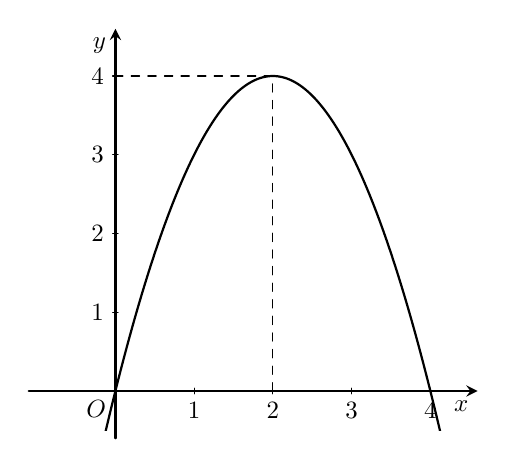
\begin{tikzpicture}[line join=round,line cap=round,>=stealth,thick]
			 \tikzset{every node/.style={scale=0.9}}
			\draw[->] (-1.1,0)--(4.6,0)  node[below left] {$x$};
			\draw[->]  (0,-0.6)--(0,4.6) node[below left] {$y$};
			\draw  (0,0) node [below left] {$O$};
			 \foreach \x/\nx in {1/1,2/2,3/3,4/4}
			\draw[thin]  (\x,1pt)--(\x,-1pt) node [below] {$\nx$};
			\foreach \y/\ny  in {1/1,2/2,3/3,4/4}
			\draw[thin] (1pt,\y)--(-1pt,\y) node [left] {$\ny$}; 
			\draw[dashed,thin](2,0)--(2,4)--(0,4); 
			\begin{scope}
				\clip  (-1,-0.5) rectangle (4.5,4.5);
				 \draw[samples=200,domain=-1:4.5,smooth,variable=\x] plot (\x,{-1*(\x)^2+4*(\x)+0});
			\end{scope}
		\end{tikzpicture}
	} 
	\shortans{399} 
	 \loigiai{
		Đồ thị là một parabol nên hàm số  có dạng $y=a x^2+b x+c$. Ta thấy đồ thị đi qua các điểm $(0; 0),(2; 4)$ và $(4; 0)$ nên ta có
		$$\heva{&c = 0\\&4 a + 2 b + c = 4\\&1 6 a + 4 b +  c = 0}\Leftrightarrow\heva{&a=-1\\&b=4\\&c=0.}$$
		Vậy $a+100b+c  = -1 + 100\cdot 4+0=399$.
	} 
\end{bt}

% từ: cau-hoi/lop10/0D3_Ham_so_bac_hai_va_do_thi/0D3-2-2_Bang_bien_thien_tinh_don_dieu_max_min.tex
\begin{ex}%[0D3Y2-2]%[ma:8f2e1c04]
	 \immini{
	Cho hàm  số $y=f(x)=ax^2+bx+c$ có đồ thị như hình vẽ.
	 Hàm số $f(x)<0$ với mọi $x$ thuộc khoảng?
	 \choice
		{$\left(4;5\right)$} 
		{$\left(-1;4\right)$} 
		{$\left(0;1\right)$} 
		{\True $\left(1;4\right)$}} 
		{\begin{tikzpicture}[scale=.5,>=stealth,font=\footnotesize,line join=round,line cap=round]
		\def\a{1} \def\b{-5}  \def\c{4}
		 \def\xmin{-1} \def\xmax{6}
		\def\ymin{-3} \def\ymax{6} 
		\draw[->] (\xmin,0)--(\xmax,0)  node [below]{$x$};
		\draw[->]  (0,\ymin)--(0,\ymax) node [left]{$y$};
		\node at  (0,0) [below left]{$O$};
		 \draw (1,0) node[above right] {$1$};
		\draw (4,0) node[above right] {$4$}; 
		\draw (0,4) node[above right]  {$4$};
		\clip (\xmin+0.1,\ymin+0.1) rectangle  (\xmax-0.5,\ymax-0.1);
		\draw[smooth,samples=300][domain=-1:6] plot  (\x,{\a*(\x)^2+\b*(\x)+\c});
	\end{tikzpicture}
		} 
	\loigiai{Dựa vào đồ thị  ta có $f(x)<0\Leftrightarrow x\in\left(1;4\right)$
	 }
\end{ex}

% từ: cau-hoi/lop10/0D3_Ham_so_bac_hai_va_do_thi/0D3-2-3_Do_thi_cua_ham_so_bac_hai.tex
\begin{ex}%[0D3H2-3]%[ma:195a4e58]
	\immini[thm]{Cho hàm số $y=a{x^2}+bx+c$ có đồ thị như bên. 
	 Khẳng định nào dưới đây là đúng?
	\choice 
		 {$a > 0,b > 0,c < 0$}
		{$a < 0,b < 0,c  > 0$}
		{$a > 0,b < 0,c >  0$}
		{\True $a > 0,b < 0,c  < 0$}
		}{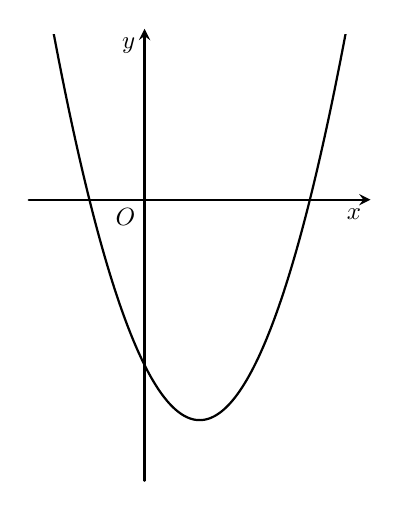
\begin{tikzpicture}[line join=round,line cap=round,>=stealth,thick,scale=0.7]
		\tikzset{every node/.style={scale=0.9}} 
		\draw[->]  (-2.1,0)--(4.1,0) node[below left] {$x$};
		 \draw[->] (0,-5.1)--(0,3.1) node[below left] {$y$};
		\draw  (0,0) node [below left] {$O$};
		\begin{scope}
			\clip  (-2,-5) rectangle (4,3);
			\draw[samples=200,domain=-2:4,smooth,variable=\x]  plot (\x,{1*(\x)^2+-2*(\x)+-3});
		\end{scope}
	\end{tikzpicture}
		} 
	\loigiai{ 
		Đồ thị  cắt trục tung tại điểm có tung độ âm nên $c < 0$.\\
		Đồ thị hướng bề lõm lên trên nên $a > 0$, hoành  độ đỉnh dương nên $\dfrac{-b}{2a}> 0, \,a > 0\Rightarrow b < 0$.
	} 
\end{ex}

% từ: cau-hoi/lop10/0D3_Ham_so_bac_hai_va_do_thi/0D3-2-3_Do_thi_cua_ham_so_bac_hai.tex
\begin{ex}%[0D3H2-3]%[ma:4d33ccde]
	Cho hàm số  $y=x^2-3x$. Hỏi hình nào sau đây là đồ thị của hàm số đã cho?
	\choice 
		{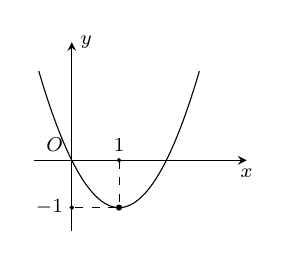
\begin{tikzpicture}[smooth,samples=300,scale=0.6,>=stealth,font=\footnotesize]
		\draw[->] (-0.8,0)--(3.7,0) node[below]{$x$}; 
		\draw[->]  (0,-1.5)--(0,2.5) node[right]{$y$};
		\draw (0,0)  node[above left]{$O$};
		\draw[domain=-0.7:2.7]  plot (\x,{(\x+1)^2-4*(\x+1)+3});
		\draw[fill=black] (1,-1) circle  (1.5pt)
			 (1,0) circle (1pt)
			(0,-1) circle (1pt); 
		\draw[dashed]  (1,0) node[above]{$1$}--(1,-1)--(0,-1) node[left]{$-1$};
	\end{tikzpicture}
		 }
		{\True 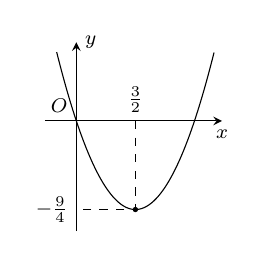
\begin{tikzpicture}[smooth,samples=300,scale=0.5,>=stealth,font=\footnotesize]
		\draw[->] (-0.8,0)--(3.7,0) node[below]{$x$}; 
		\draw[->]  (0,-2.8)--(0,2) node[right]{$y$};
		\draw (0,0)  node[above left]{$O$};
		 \draw[domain=-0.5:3.5] plot (\x,{(\x)^2-3*(\x)});
		\draw[fill=black] (1.5,-2.25) circle (1.5pt); 
		\draw[dashed] (1.5,0) node[above]{$\frac{3}{2}$}--(1.5,-2.25)--(0,-2.25) node[left]{$-\frac{9}{4}$}; 
	\end{tikzpicture}
		} 
		{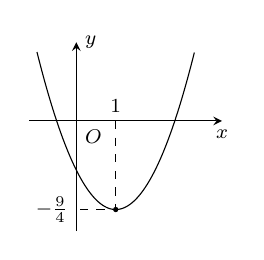
\begin{tikzpicture}[smooth,samples=300,scale=0.5,>=stealth,font=\footnotesize]
		\draw[->]  (-1.2,0)--(3.7,0) node[below]{$x$};
		 \draw[->] (0,-2.8)--(0,2) node[right]{$y$};
		\draw (0,0)  node[below right]{$O$};
		 \draw[domain=-1:3] plot (\x,{(\x+0.5)^2-3*(\x+0.5)});
		\draw[fill=black]  (1,-2.25) circle (1.5pt);
		\draw[dashed]  (1,0) node[above]{$1$}--(1,-2.25)--(0,-2.25) node[left]{$-\frac{9}{4}$};
	\end{tikzpicture}
		 }
		{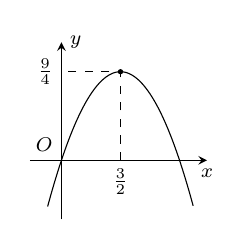
\begin{tikzpicture}[smooth,samples=300,scale=0.5,>=stealth,font=\footnotesize]
		\draw[->] (-0.8,0)--(3.7,0) node[below]{$x$}; 
		\draw[->] (0,-1.5)--(0,3)  node[right]{$y$};
		\draw (0,0) node[above left]{$O$}; 
		\draw[domain=-0.35:3.35]  plot (\x,{-(\x)^2+3*(\x)});
		\draw[fill=black] (1.5,2.25) circle  (1.5pt);
		\draw[dashed] (1.5,0)  node[below]{$\frac{3}{2}$}--(1.5,2.25)--(0,2.25) node[left]{$\frac{9}{4}$};
	\end{tikzpicture}
		} 
	\loigiai{ 
		Tọa độ đỉnh của parabol là $I\left(\dfrac{-b}{2a};\dfrac{-\Delta}{4a}\right)=I\left(\dfrac{3}{2};\dfrac{-9}{4}\right)$. 
	 }
\end{ex}

% từ: cau-hoi/lop10/0D3_Ham_so_bac_hai_va_do_thi/0D3-2-3_Do_thi_cua_ham_so_bac_hai.tex
\begin{ex}%[0D3Y2-3]%[ma:46c0a228]
	Cho hàm số $y=x^2-3x$. Hỏi hình nào sau  đây là đồ thị của hàm số đã cho?
	\choice 
		{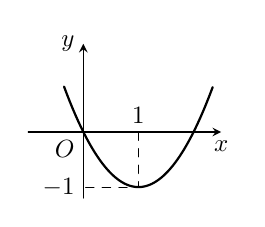
\begin{tikzpicture}[>=stealth,scale=0.7,line join=round,line cap=round]
		\draw[->]  (-1,0)--(2.5,0) node [below]{$x$};
		\draw[->]  (0,-1.2)--(0,1.6) node [left]{$y$};
		\node at  (0,0) [below left]{$O$};
		\clip; 
		\draw[smooth,samples=300,domain=-0.35:2.35,thick]  plot (\x,{(\x)^2-2*(\x)});
		\draw[dashed](1,0) node[above]{$1$}--(1,-1)--(0,-1) node[left]{$-1$}; 
	\end{tikzpicture}
		} 
		{\True 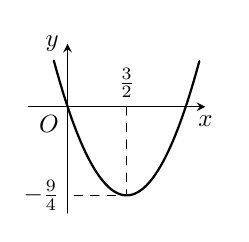
\begin{tikzpicture}[>=stealth,scale=0.5,line join=round,line cap=round]
		\draw[->] (-1,0)--(3.5,0) node [below]{$x$}; 
		 \draw[->] (0,-2.7)--(0,1.6) node [left]{$y$};
		\node at (0,0) [below left]{$O$}; 
		\clip; 
		 \draw[smooth,samples=300,domain=-0.35:3.35,thick] plot (\x,{(\x)^2-3*(\x)});
		\draw[dashed](3/2,0)  node[above]{$\frac{3}{2}$}--(3/2,-9/4)--(0,-9/4) node[left]{$-\frac{9}{4}$};
	\end{tikzpicture}
		 }
		{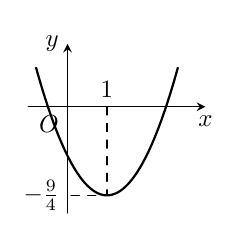
\begin{tikzpicture}[>=stealth,scale=0.5,line join=round,line cap=round]
		 \draw[->] (-1,0)--(3.5,0) node [below]{$x$};
		\draw[->] (0,-2.7)--(0,1.6) node [left]{$y$}; 
		\node at (0,0)  [below left]{$O$};
		\clip; 
		\draw[smooth,samples=300,domain=-0.8:2.8,thick] plot (\x,{(\x)^2-2*(\x)-5/4}); 
		\draw[dashed](1,0)  node[above]{$1$}--(1,-9/4)--(0,-9/4) node[left]{$-\frac{9}{4}$};
	\end{tikzpicture}
		} 
		{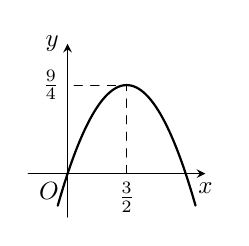
\begin{tikzpicture}[>=stealth,scale=0.5,line join=round,line cap=round]
		 \draw[->] (-1,0)--(3.5,0) node [below]{$x$};
		\draw[->] (0,-1.1)--(0,3.3) node [left]{$y$}; 
		\node at (0,0) [below  left]{$O$};
		\clip; 
		\draw[smooth,samples=300,domain=-0.25:3.25,thick]  plot (\x,{-(\x)^2+3*(\x)});
		\draw[dashed](3/2,0) node[below]{$\frac{3}{2}$}--(3/2,9/4)--(0,9/4)  node[left]{$\frac{9}{4}$};
	\end{tikzpicture}
		 }
	 \loigiai{
		Đồ thị hàm số $y=x^2-3x$ có $a=1>0$ và đỉnh  có tọa độ là $\left(\dfrac{3}{2}; -\dfrac{9}{4}\right)$ nên ta chọn phương án parabol có bề lõm hướng lên và đỉnh có tọa độ là $\left(\dfrac{3}{2}; -\dfrac{9}{4}\right)$.
	} 
\end{ex}

% từ: cau-hoi/lop10/0D3_Ham_so_bac_hai_va_do_thi/0D3-2-3_Do_thi_cua_ham_so_bac_hai.tex
\begin{bt}%[0D3H2-3]%[ma:2e0ae82e]
	\immini
	{
		Xác định dấu của các hệ số $a, b, c$ và dấu của biệt thức $\Delta=b^2-4 a c$ của hàm số bậc hai $y=a x^2+b x+c$, biết đồ thị của nó có dạng như hình bên.
	}
	{
		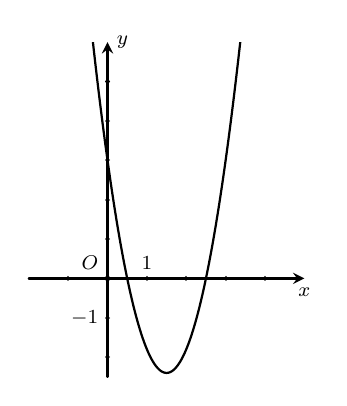
\begin{tikzpicture}[join=round, cap=round,>=stealth,thick, font = \footnotesize, scale = .5]
			\def \xmin{-2} 		\def \xmax{5}
			\def \ymin{-2.5}	\def \ymax{6}
			\def \hamso{(12/5)*(\x)^2 - (36/5)*(\x) + 3}
			\draw[->] (\xmin,0)--(\xmax,0) node[below] {$x$}; 
			\draw[->] (0,\ymin)--(0,\ymax) node[right] {$y$}; 
			\fill (0,0) circle (2pt) node [above left] {$O$}; 
			\foreach \x in {-1,1,2,3,4} 
			\draw(\x,1pt)--(\x,-1pt); 
			\foreach \y in {-2,-1,1,2,3,4,5} 
			\draw(1pt,\y)--(-1pt,\y);
			\path (1,0) node[above]{$1$} 
			(0,-1) node[left]{$-1$};
			\begin{scope}
				\clip (\xmin+0.01,\ymin+0.01) rectangle (\xmax-0.01,\ymax-0.01); 
				\draw plot[samples=350,domain=\xmin+0.01:\xmax-0.01,smooth,variable=\x] (\x,{\hamso});
			\end{scope}
		\end{tikzpicture}
	}
	\loigiai
	{
		Từ đồ thị của hàm số ta thấy:
		\begin{itemize}
			\item Đồ thị quay bề lõm lên trên nên $a>0$.
			\item Đồ thị cắt trục tung tại điểm có tung độ dương nên $c>0$.
			\item Hoành độ đỉnh $x=-\dfrac{b}{2 a}$ có giá trị dương nên $a$ và $b$ trái dấu. Vì $a>0$ nên $b<0$.
		\end{itemize}
		Mặt khác, vì đồ thị hàm số cắt trục hoành $O x$ tại hai điểm phân biệt, tức là phương trình $a x^2+b x+c=0$ có hai nghiệm phân biệt nên $\Delta=b^2-4 a c>0$. \\
		Vậy $a>0, b<0, c>0$ và $\Delta=b^2-4 a c>0.$
	}
\end{bt}

% từ: cau-hoi/lop10/0D3_Ham_so_bac_hai_va_do_thi/0D3-2-6_Toan_thuc_te_ung_dung_ham_so_bac_hai.tex
\begin{bt}%[0D3V2-6]%[ma:4c6de71b]
	Một vật chuyển động trong $3$ giờ với vận tốc $v$ (km/h) phụ thuộc vào thời gian $t(h)$ có đồ thị của hàm số vận tốc như hình bên dưới. Trong khoảng thời gian một giờ từ khi vật bắt đầu chuyển động, đồ thị đó là một phần parabol có đỉnh $I(2;9)$ và trục đối xứng song song với trục tung, khoảng thời gian còn lại đồ thị là một đoạn thẳng song song với trục hoành. Tính vận tốc của vật tại thời điểm $t=2$.
	\begin{center}
		\begin{tikzpicture}[scale=0.7, font=\footnotesize, line join=round, line cap=round, >=stealth]
			\def\xmin{-1}\def\xmax{5}\def\ymin{-1}\def\ymax{10}
			\draw[->] (\xmin-0.2,0)--(\xmax+0.2,0) node[below] {\footnotesize $x$};
			\draw[->] (0,\ymin-0.2)--(0,\ymax+0.2) node[right] {\footnotesize $y$};
			\draw (0,0) node [below left] {\footnotesize $O$};
			\foreach \x in {1,2,3}\draw (\x,0.1)--(\x,-0.1) node [below] {\footnotesize $\x$};
			\foreach \y in {4,9}\draw (0.1,\y)--(-0.1,\y) node [left] {\footnotesize $\y$};
			\clip (0,\ymin) rectangle (\xmax,\ymax);
			\draw[smooth,samples=200,domain=\xmin:1] plot (\x,{-1.25*((\x)^2)+5*\x+4});
			\draw[dashed,smooth,samples=200,domain=1:3] plot (\x,{-1.25*((\x)^2)+5*\x+4});
			\draw[dashed] (2.0,0)--(2.0,9.0)--(0,9.0);\fill (2.0,9.0) circle (1pt);
			\draw[dashed] (1,31/4)--(1,0);
			\draw[dashed] (3,31/4)--(3,0);
			\draw (1,31/4)--(3,31/4);
		\end{tikzpicture}
	\end{center}
	\loigiai{
	Gọi phương trình của parabol là $v(t)=a t^2+b t+c$ $(a \neq 0)$.\\
	Vì parabol đi qua điểm có tọa độ $(0 ; 4)$ và có đỉnh $I(2 ; 9)$ nên ta có hệ phương trình
	$$\heva{&-\dfrac{b}{2a}=2\\&4a+2b+c=9 \\&c=4}\Leftrightarrow\heva{&4 a+b=0\\&4a+2b+c=9\\&c=4}\Leftrightarrow\heva{&a=-\dfrac{5}{4}\\&b=5\\&c=4.}$$
	Do đó $v(t)=-\dfrac{5}{4} t^2+5 t+4$.\\
	Vì trong khoảng thời gian từ $1$ đến $3$ giờ đồ thị vận tốc là một đoạn thẳng song song với trục hoành nên $v(2)=v(1)=\dfrac{31}{4}$.	
	}
\end{bt}

% từ: cau-hoi/lop10/0D7_Bat_phuong_trinh_bac_2_mot_an/0D7-1-4_Xet_dau_bieu_thuc_dang_tich_thuong.tex
\begin{ex}%[0D7H1-4]%[ma:6947e064]
	Tìm  tập nghiệm của bất phương trình $\dfrac{x^{2}-3x-4}{x-1}\leq 0$.
	\choice 
		 {$T=(-\infty;-1]\cup[1;4]$}
		 {\True $T=(-\infty;-1]\cup(1;4]$}
		 {$T=(-\infty;-1)\cup(1;4]$}
		{$T=(-\infty;-1]\cup(1;4)$} 
	 \loigiai{
		Xét biểu  thức $f(x)=\dfrac{x^{2}-3x-4}{x-1}$.\\
		 Ta có
		\begin{itemize}
			 \item $x^{2}-3 x-4=0\Leftrightarrow\hoac{&x=-1\\&x=4.}$
			\item $x-1=0 \Leftrightarrow  x=1$.
		\end{itemize}
		Bảng xét dấu 
		\begin{center}
			
\begin{tikzpicture}
					 \tkzTabInit[nocadre=true,lgt=2.5,espcl=2,deltacl=0.5]
						{$x$/0.7,$x^2-3x-4$/0.7,$x-1$/.7,$f  (x)$/.7}
						{$-\infty$,$-1$,$1$,$4$,$+\infty$} 
					 \tkzTabLine{,+,$0$,-,|,-,$0$,+,}
					\tkzTabLine{,-,|,-,0,+,|,+,} 
					\tkzTabLine{,-,$0$,+,||,-,$0$,+,} 
				\end{tikzpicture}
		\end{center}
		Từ bảng xét dấu, suy ra  $f(x)\leq0\Leftrightarrow x\in (-\infty;-1]\cup(1;4]$.\\
		Vậy tập nghiệm của bất phương  trình đã cho là $T=(-\infty;-1]\cup(1;4]$.
	} 
\end{ex}

% từ: cau-hoi/lop10/0D7_Bat_phuong_trinh_bac_2_mot_an/0D7-2-6_Bai_toan_co_tham_so.tex
\begin{bt}%[Bài Giảng K10-K11, Đỗ Viết Lân]%[0D7V2-6]%[ma:efc4c384]
	Tìm $m$ để phương trình $2x^2+(m+1)x+m+8=0$ có nghiệm.
	\loigiai{
		Ta có $2x^2+(m+1)x+m+8=0$ là phương trình bậc hai một ẩn. \\
		Vậy phương trình có nghiệm khi và chỉ khi
		$\Delta = m^2 -6m -63 \ge 0$. Khi đó $m=3-6\sqrt{2}$ hoặc $m=3+6\sqrt{2}$.
	}
\end{bt}

% từ: cau-hoi/lop10/0D7_Bat_phuong_trinh_bac_2_mot_an/0D7-2-6_Bai_toan_co_tham_so.tex
\begin{bt}%[0D7V2-6]%[Dự án đề kiểm tra GHKII NH22-23- Dương Phước Sang]%[Marie Curie]%[ma:332207d2]
		Tìm tất cả các giá trị của tham số $m$ để hàm số $f(x)=(3m+1){x^2}-(3m+1)x+m+4$ là tam thức bậc hai âm với mọi $x\in \mathbb{R}$.
		\loigiai{
			\textbf{Trường hợp 1:} $3m+1=0 \Leftrightarrow m=-\dfrac{1}{3} $ thì $ f(x)=\dfrac{11}{3}>0 $ với mọi $x\in \mathbb{R}$.\\
			Như thế, $ m= -\dfrac{1}{3}$ không thỏa mãn yêu cầu của bài toán.\\
			\textbf{Trường hợp 2:} $ m \neq -\dfrac{1}{3} $ thì yêu cầu bài toán xảy ra khi và chỉ khi 
			$$\heva{&a<0\\&\Delta <0} 
			\Leftrightarrow
			\heva{&3m+1<0\\&(3m+1)^2-4(3m+1)(m+4)<0}
			\Leftrightarrow \heva{&m<-\dfrac{1}{3}\\&\hoac{&m<-15\\&m>-\dfrac{1}{3}}}\Leftrightarrow m<-15.$$
		}
	\end{bt}

% từ: cau-hoi/lop10/0D8_Dai_so_to_hop/0D8-3-2_Khai_trien_mot_nhi_thuc_Newton.tex
\begin{bt}%[0D8H3-2]%%[Dự án đề kiểm tra HKII NH22-23- Nguyễn Mộng Hùng]%[Nguyễn Thị Diệu]%[ma:0b91f06a]
	Khai triển và rút gọn biểu thức sau $T=x\left(2-3x\right)^4$
	\loigiai{
	Ta có 
	\allowdisplaybreaks
	\begin{eqnarray*}
		T&=&x\left(2-3x\right)^4\\
		 &=&x\left[2+(-3x)\right]^4\\
		 &=&x\left[\mathrm{C}_4^0\cdot 2^4+\mathrm{C}_4^1\cdot 2^3\cdot(-3x)+\mathrm{C}_4^2\cdot 2^2\cdot(-3x)^2+\mathrm{C}_4^3\cdot 2\cdot(-3x)^3+\mathrm{C}_4^4\cdot(-3x)^4\right]\\
		 &=&x\left[16-96x+216x^2-216x^3+81x^4\right]\\
		 &=&16x-96x^2+216x^3-216x^4+81x^5.
	\end{eqnarray*}

}
\end{bt}

% từ: cau-hoi/lop10/0H4_He_thuc_luong_trong_tam_giac/0H4-1-2_Tinh_cac_gia_tri_luong_giac.tex
\begin{ex}%[0H4H1-2]%[ma:d8c19b46]
	Tính giá trị của biểu thức $A=\sin (10^{\circ})\cdot \sin (20^{\circ})\ldots \sin (190^{\circ})\cdot \sin (200^{\circ})$. 
	\choice 
		{$4$} 
		{$2$} 
		 {\True $0$}
		{$-2$} 
	 \loigiai{
		Ta thấy trong tích có $\sin 180^{\circ}=0$ và do đó  $A=0$.
	} 
\end{ex}

% từ: cau-hoi/lop10/0H4_He_thuc_luong_trong_tam_giac/0H4-1-2_Tinh_cac_gia_tri_luong_giac.tex
\begin{bt}[Mức độ 2]%[Nguyễn Trung Kiên, dự án bài giảng 10-11, CTGDPT2018]%[0H4H1-2]%[ma:848bcf72]
	Tính giá trị của biểu thức $A=3-\sin^2{90^\circ}+2\cos^2{60^\circ}-3\tan^2{45^\circ}$.
	\loigiai
	{Ta có $\sin90^\circ=1$, $\cos60^\circ=\dfrac{1}{2}$, $\tan45^\circ=1$ nên
		\allowdisplaybreaks
		\begin{align*}
			A=&\, 3-\sin^2{90^\circ}+2\cos^2{60^\circ}-3\tan^2{45^\circ}\\
			=&\, 3-\left(\sin90^\circ\right)^2 + 2\left(\cos60^\circ\right)^2 - 3\left(\tan45^\circ\right)^2\\
			=&\, 3-1^2+2\left(\dfrac{1}{2}\right)^2-3\cdot 1^2\\
			=&\, -\dfrac{1}{2}.
	\end{align*}}
\end{bt}

% từ: cau-hoi/lop10/0H4_He_thuc_luong_trong_tam_giac/0H4-2-1_Bai_toan_chi_dung_dinh_ly_Sin_Cosin.tex
\begin{ex}%[0H4H2-1]%[0H4H2-1]%[ma:9fce14f5]
	Cho tam giác $ABC$ thỏa  mãn hệ thức $b+c=2a$. Mệnh đề nào sau đây là đúng?
	\choice 
		{$\cos B+\cos C=2\cos A$} 
		 {\True $\sin B+\sin C=2\sin A$}
		{$\sin B+\sin C=\dfrac{1}{2}\sin A$} 
		 {$\sin B+\cos C=2\sin A$}
	\loigiai{ 
		Ta có $b+c=2a$ $\Leftrightarrow 2R\sin B+2R\sin C=2\cdot 2R\sin  A$ $\Leftrightarrow\sin B+\sin C=2\sin A$.
	} 
\end{ex}

% từ: cau-hoi/lop10/0H4_He_thuc_luong_trong_tam_giac/0H4-2-1_Bai_toan_chi_dung_dinh_ly_Sin_Cosin.tex
\begin{bt}%[24-25 Bài giảng K10-K11, Phan Chiến Thắng]%[0H4H2-1]%[ma:509cd0f2]
	\immini{
		Cho tam giác $ABC$ có $\widehat{A}= 40^\circ$, $\widehat{B}=55^\circ$ và $AB = 100$. Tính độ dài cạnh $BC$ (làm tròn kết quả đến hàng phần mười).
	}
	{
		\begin{tikzpicture}[scale=1, font=\footnotesize, line join=round, line cap=round,>=stealth]
			\path
			(0,0) coordinate (A)
			(4,0) coordinate (B)
			;
			\coordinate (A') at ($(A)+(40:3)$); 
			\coordinate (B') at ($(B)+(-55:3)$); 
			\coordinate (C) at (intersection of A--A' and B--B');
			\draw (A)--(B)--(C)--(A);
			
			\tkzMarkAngle[arc=ll,size=0.5,mark=0](B,A,C)
			\tkzLabelAngle[pos=1.1](B,A,C) {$40^\circ$}
			\tkzMarkAngle[arc=l,size=0.5,mark=0](C,B,A)
			\tkzLabelAngle[pos=0.8](C,B,A) {$55^\circ$}
			\foreach \x/\g in {A/-120,B/-60,C/90} 
			\fill[black] (\x) circle (1pt)+(\g:3mm) node {$\x$};
		\end{tikzpicture}
	}
	\loigiai{
		Ta có $\widehat{C}= 180^\circ -  \widehat{A} -\widehat{B} = 180^\circ - 40^\circ-55^\circ  =85^\circ$. \\
		Áp dụng định lí sin ta có 
		\[
		\dfrac{AB}{\sin C} = \dfrac{BC}{\sin A} \Rightarrow BC = \dfrac{AB\sin A}{\sin C}  = \dfrac{100\sin 40^{\circ}}{\sin 85^{\circ}} \approx 64{,}5. 
		\]
	}
\end{bt}

% từ: cau-hoi/lop10/0H4_He_thuc_luong_trong_tam_giac/0H4-2-1_Bai_toan_chi_dung_dinh_ly_Sin_Cosin.tex
\begin{bt}%[0H4H2-1] % KIEM_TRA%[0H7GK-1]%[Dự án đề kiểm tra HKII đợt 1- Vũ Ngọc Hảo]%[THPTChuyenLeHongPhong]%[ma:5e62bec1]
\immini{	Tính bán kính đường tròn trong hình vẽ trên biết hình vuông có cạnh 
bằng $2$.}{
	\begin{tikzpicture}
\def\r{2.304886114323222}
\path
(0,0) coordinate (A)
(0,1) coordinate (B)
(1,0) coordinate (C)
(1,2) coordinate (D)
(2,2) coordinate (E)
(2,1) coordinate (K)
(2,3) coordinate (G)
(3,3) coordinate (I)
(3,2) coordinate (F)
(4,2) coordinate (M)
(4,1) coordinate (N)
(3,1) coordinate (L)
(3,2) coordinate (F)
(1.75,1.5) coordinate (O)
($(M)!0.5!(N)$)coordinate (H);
\draw[black] (O) circle (\r);
\draw 
(A)--(B)--(K)--(G)--(I)--(L)--(N)--(L)  (A)--(C)--(D)--(M)--(N);
\draw [fill=black] (A) circle (.05);
\draw [fill=black] (B) circle (.05);
\draw [fill=black] (C) circle (.05);
\draw [fill=black] (D) circle (.05);
\draw [fill=black] (E) circle (.05);
\draw [fill=black] (K) circle (.05);
\draw [fill=black] (G) circle (.05);
\draw [fill=black] (I) circle (.05);
\draw [fill=black] (F) circle (.05);
\draw [fill=black] (M) circle (.05);
\draw [fill=black] (N) circle (.05);
\draw [fill=black] (L) circle (.05);
\draw [fill=black] (F) circle (.05);
\draw [fill=black] (1,1) circle (.05);
\end{tikzpicture}
}
\loigiai{
\immini{Xét tam giác $ABC$ nội tiếp đường tròn có:\\
$BC=2$ (cạnh hình vuông)\\
$AC=\sqrt{(a\cdot 2)^2+(2\cdot 2)^2}=4\sqrt{5}$ (pytago)\\
$AB=\sqrt{(a\cdot 2)^2+(1\cdot 2)^2}=2\sqrt{17}$ (pytago)\\
$S_{ABC}=\dfrac{1}{2}\cdot BC\cdot DC=\dfrac{1}{2}\cdot 2\cdot (4\cdot 2)=8$ do $DC=d(A;BC)$\\
Mà $S_{ABC}=\dfrac{AB\cdot AC\cdot BC}{4R}$\\
Vậy $R_{(ABC)}=\dfrac{AB\cdot AC\cdot BC}{4S_{ABC}}=\dfrac{2\sqrt{17}\cdot 4\sqrt{5}\cdot 2}{4\cdot 8}=\dfrac{\sqrt{85}}{2}$}
		{\begin{tikzpicture}
\def\r{2.304886114323222}
\path
(0,0) coordinate (A)
(0,1) coordinate (N)
(1,0) coordinate (M)
(1,2) coordinate (Z)
(2,2) coordinate (E)
(2,1) coordinate (K)
(2,3) coordinate (G)
(3,3) coordinate (I)
(3,2) coordinate (F)
(4,2) coordinate (C)
(4,1) coordinate (B)
(3,1) coordinate (L)
(3,2) coordinate (F)
(1.75,1.5) coordinate (O)
(0,2) coordinate (D)
($(M)!0.5!(N)$)coordinate (H);
\draw[black] (O) circle (\r);
\draw 
(A)--(N)--(K)--(G)--(I)--(L)--(B)--(L)  (A)--(M)--(Z)--(C)--(B);
\draw[red] (A)--(B)--(C)--(A);
\draw[dashed] (0,1)--(0,2)--(1,2) (2,1)--(3,1);
\draw [fill=black] (Z) circle (.05);
\draw [fill=black] (E) circle (.05);
\draw [fill=black] (K) circle (.05);
\draw [fill=black] (G) circle (.05);
\draw [fill=black] (I) circle (.05);
\draw [fill=black] (F) circle (.05);
\draw [fill=black] (M) circle (.05);
\draw [fill=black] (N) circle (.05);
\draw [fill=black] (L) circle (.05);
\draw [fill=black] (F) circle (.05);
\draw [fill=black] (1,1) circle (.05);
\draw [fill=black] (0,2) circle (.05);
	\foreach \x/\g in {A/180,B/0,C/0,D/90}
\draw [fill= black] (\x) circle (.05)+(\g:.3) node{$\x$};
	\end{tikzpicture}}
}
\end{bt}

% từ: cau-hoi/lop10/0H4_He_thuc_luong_trong_tam_giac/0H4-2-2_Bai_toan_co_dung_cong_thuc_dien_tich.tex
\begin{bt}%[0H4V2-2]%[Dự án đề kiểm tra Toán 10 GHKI NH23-24- Đỗ Đường Hiếu]%[THPT ]%[ma:92febc2f]
	\immini{Cho tam giác $ABC$ có $AB=4$, $BC=6$, $\widehat{ABC}=120^\circ$ (tham khảo hình vẽ). Tính độ dài cạnh $AC$ và độ dài đường cao $BH$ của tham giác $ABC$.}
	{\begin{tikzpicture}[scale=1, line cap=round,line join=round,font=\footnotesize]
			\path
			(0:0) coordinate (A)
			(0:4) coordinate (C)
			(46.5:2) coordinate (B)
			($(A)!(B)!(C)$) coordinate (H)
			;
			\draw (A)--(B)--(C)--cycle (B)--(H)
			;
			\pic [draw, angle eccentricity=1.5] {angle = A--B--C};
			\foreach \x/\g in {A/180,B/90,C/0,H/-90} \draw[fill=black] (\x) circle (.05) +(\g:.3) node {$\x$}
			;
	\end{tikzpicture}
}
	\loigiai{
	\begin{itemize}
		\item $AC^2=AB^2+BC^2-2\cdot AB\cdot BC \cos \widehat{ABC}=4^2+6^2-2\cdot 4\cdot 6\cdot \cos 120^\circ=76$.\\
		Suy ra $AC=2\sqrt{19}$.
		\item $S_{\triangle ABC}=\dfrac{1}{2}AB\cdot BC\cdot\sin \widehat{ABC}=120^\circ=\dfrac{1}{2}\cdot 4\cdot 6\cdot \sin 120^\circ=6\sqrt{3}$.\\
		Do đó, độ dài đường cao $BH$ là $BH=\dfrac{2S_{\triangle ABC}}{AC}=\dfrac{2\cdot 6\sqrt{3}}{2\sqrt{19}}=\dfrac{6\sqrt{57}}{19}$.
	\end{itemize}
	}
\end{bt}

% từ: cau-hoi/lop10/0H4_He_thuc_luong_trong_tam_giac/0H4-2-2_Bai_toan_co_dung_cong_thuc_dien_tich.tex
\begin{bt}%[0H4H2-2]%[Tex hóa SGK CD-CT,T7/22, Phạm Tiến Long]%[ma:3ac90540]
	Tính diện tích một cánh buồm hình tam giác có chiều dài một cạnh là $3{,}2$ m và hai góc kề cạnh đó có số đo lần lượt là $48^\circ$ và $105^\circ$. (xem hình bên dưới).
	\begin{center}
		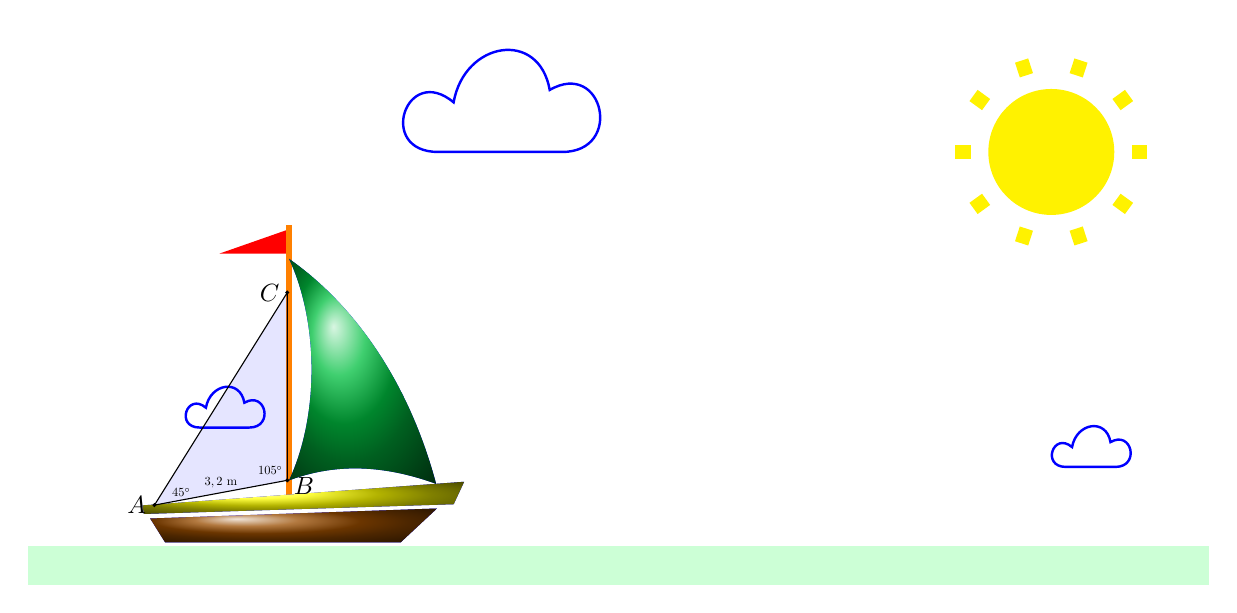
\begin{tikzpicture}[transform shape, scale=0.5]
			\tikzset{Icon-mattroi/.pic={
					\def\r{0.35}
					\fill(0,0)circle(\r);
					\draw[line width=2*\r pt](0,0)circle(\r);
					\foreach \g in{1,...,10}{
						\draw[line width=5 pt](\g*36:1.2*\r)++(\g*36:0.1*\r)--++(\g*36:\r*0.25);
					}
			}}
			\tikzset{Icon-may/.pic={
					\def\r{0.35}
					\draw[line width=2.5*\r pt](-\r,0)--(\r,0)..controls++(0:\r) and ++(30:\r)..(0.8*\r,\r)..controls++(100:\r) and ++(80:\r)..(-0.75*\r,0.8*\r)..controls++(140:\r) and++(180:\r)..(-\r,0);
			}}
			\fill[green!80!cyan,opacity=0.2](-10,-4)rectangle(20,-5);
			\tikzset{thuyen/.pic={
					\fill[red](-0.36,3.8)--++(180:2)--(-0.36,4.5)--cycle;
					\draw[orange,line width=2pt](-0.4,-3.2)--++(90:7.8);
					\fill[ball color=orange!60!black](-3.9,-4.35)--(2.75,-4.35)--++(43:1.4)--++(182:8.1)--cycle;
					\fill[ball color=yellow](-4.5,-3.55)--++(1.8:8.75)--++(65:0.7)--++(184.2:9.1)--cycle;
					\fill[opacity=0.1](-4.2,-3.3)coordinate(A)--(-0.45,2.7)coordinate(C)--(-0.45,-2.6)coordinate(B)--cycle;
					\fill[ball color=teal!50!green](-0.4,-2.6)..controls++(20:1) and++(160:2)..(3.75,-2.7)..controls++(105:3.25) and++(-35:2)..(-0.4,3.65)..controls++(-65:2) and++(65:2)..(-0.4,-2.6);
			}}
			\path(-3,0)pic[blue]{thuyen}(16,6)pic[yellow,scale=5]{Icon-mattroi}(2,6)pic[scale=5][blue]{Icon-may}(-5,-1)pic[scale=2][blue]{Icon-may}(17,-2)pic[scale=2][blue]{Icon-may};
			\draw(A)--(C)--(B)--cycle (A)--(B)
			node[pos=.5,above]{$3,2$ m};
			\foreach \d/\g in{A/180,B/-20,C/180}
			\draw[fill=black](\d)circle(1pt)node[shift={(\g:0.5)},scale=2]{$\d$};
			\tkzMarkAngles[pos=0.5](B,A,C C,B,A)
			\path(A)++(25:0.75)node{$45^\circ$}(B)++(150:0.5)node{$105^\circ$};
		
\end{tikzpicture}
	\end{center}
	\loigiai{
		Gọi ba đỉnh của cánh buồm là $ABC$. Đặt $a=BC$; $b=AC$; $c=AB$.\\
		Ta có $c=3{,}2$ m; $\widehat{C}=180^\circ-\left(105^\circ+48^\circ\right)=27^\circ$.\\
		Áp dụng định lí sin, ta có  $\dfrac{a}{\sin A}=\dfrac{b}{\sin B}=\dfrac{c}{\sin C}=2R$.\\
		Suy ra $AC=b=\dfrac{c\sin B}{\sin C}=\dfrac{3{,}2 \cdot \sin 105^\circ}{\sin 27^\circ} \approx 6{,}8$ m;\\
		Ta có $S=\dfrac{1}{2}bc\sin A=\dfrac{1}{2} \cdot 6{,}8 \cdot 3{,}2 \cdot \sin 48^\circ \approx 8{,}1\text{ m}^2$.}
\end{bt}

% từ: cau-hoi/lop10/0H4_He_thuc_luong_trong_tam_giac/0H4-3-1_Giai_tam_giac.tex
\begin{bt}[1,5 điểm]%[0H4H3-1]%[Dự án đề kiểm tra Toán 10 GKI NH24-25- Quan Ón]%[THPT Phạm Phú Thứ - Tp HCM]%[ma:2a763ff0]
	Cho tam giác $DEF$ có $DE = 5$, $EF = 3$ và $\widehat{E} = 120^\circ$.
	\begin{enumerate}
		\item Tính số đo góc $\widehat{D}$.
		\item Tính bán kính đường tròn nội tiếp tam giác $DEF$.
		\item Tính độ dài đường trung tuyến $DI$ của tam giác $DEF$.
	\end{enumerate}
	\loigiai{
		\begin{center}
			\begin{tikzpicture}[>=stealth,line join=round,line cap=round,font=\footnotesize,scale=1]
				\path 
				(0,0) coordinate (E)
				(5,0) coordinate (D)
				($(E) + (120:3)$) coordinate (F)
				($(E)!0.5!(F)$) coordinate (I)
				;
				\draw 
				(E)--(D)--(F)--(E) (D)--(I);
				;
				\foreach \p/\g in {E/-90, D/-90, F/90, I/180}
				\draw[fill=black] (\p) circle (1pt) node[shift=(\g:3mm)] {$\p$};
				\pic[draw,angle radius=3mm,angle eccentricity=1.5] {angle = D--E--F};
				\fill (E) node[shift=(50:5.5mm), rotate = -20] {$120^\circ$};
				\path 
				(E) edge node[midway, sloped, rotate=80, anchor=center] {$ - $} (I)
				(I) edge node[midway, sloped, rotate=80, anchor=center] {$ - $} (F);
			\end{tikzpicture}
		\end{center}
		\begin{enumerate}
			\item Xét $\triangle DEF$, áp dụng định lí côsin, ta có
			\begin{eqnarray*}
				DF^2 &=& DE^2 + EF^2 - 2DE\cdot EF\cdot \cos\widehat{DEF}\\
				&=& 5^2 + 3^2 - 2\cdot 5\cdot 3\cdot\cos 120^\circ\\
				&=& 49\\
				\Rightarrow DF &=& \sqrt{49} = 7.
			\end{eqnarray*}
			Áp dụng hệ quả định lí côsin, ta có
			$$ \cos\widehat{EDF} = \dfrac{DE^2 + DF^2 - EF^2}{2\cdot DE\cdot DF} = \dfrac{5^2 + 7^2 - 3^2}{2\cdot 5\cdot 7} = \dfrac{13}{14} $$
			$\Rightarrow \widehat{EDF} \approx 21^\circ 47'$.
			\item Ta có $p = \dfrac{1}{2}(DE + DF + EF) = \dfrac{1}{2}(5 + 7 + 3) = \dfrac{15}{2}$.\\
			Do đó $S_{\triangle DEF} = \dfrac{1}{2}DE\cdot EF\cdot\sin\widehat{DEF} = \dfrac{1}{2}\cdot 5\cdot 3\cdot\sin 120^\circ = \dfrac{15\sqrt{3}}{4}$.\\
			Mà $S_{\triangle DEF} = pr \Rightarrow r = \dfrac{S_{\triangle DEF}}{p} = \dfrac{\dfrac{15\sqrt{3}}{4}}{\dfrac{15}{2}} = \dfrac{\sqrt{3}}{2} \approx 0{,}87$.\\
			Vậy bán kính đường tròn nội tiếp tam giác $DEF$ gần bằng $0{,}87$.
			\item Vì $DI$ là đường trung tuyến của $\triangle DEF$ nên $I$ là trung điểm của $EF$.\\
			Do đó $EI = \dfrac{1}{2}EF = \dfrac{1}{2}\cdot 3 = \dfrac{3}{2}$.\\
			Xét $\triangle DEI$, áp dụng định lí côsin, ta có
			\begin{eqnarray*}
				DI^2 &=& DE^2 + EI^2 - 2\cdot DE\cdot EI\cdot\cos\widehat{DEI}\\
				&=& 5^2 + \left(\dfrac{3}{2}\right)^2 - 2\cdot 5\cdot \dfrac{3}{2}\cdot \cos 120^\circ\\
				&=& \dfrac{139}{4}\\
				\Rightarrow DI &=& \dfrac{\sqrt{139}}{2}.
			\end{eqnarray*}
		\end{enumerate}
	}
\end{bt}

% từ: cau-hoi/lop10/0H4_He_thuc_luong_trong_tam_giac/0H4-3-1_Giai_tam_giac.tex
\begin{bt}%[0H4H3-1]%[Tex hóa SGK CD-CT,T7/22, Lương Như Quỳnh]%[ma:1ea1f5d0]
	Tính các góc chưa biết của tam giác $ABC$ trong các trường hợp sau:
	\begin{listEX}
		\item $\widehat{A}=42^{\circ}$, $\widehat{B}=63^{\circ}$,
		\item $BC=10$, $AC=20$, $\widehat{C}=80^{\circ}$,
		\item $AB=15$, $AC=25$, $BC=30$.
	\end{listEX}
	\loigiai{
		Đặt $a=BC$, $b=AC$, $c=AB$.
		\begin{listEX}
			\item Ta có $ \widehat{C}=180^\circ - \widehat{A}-\widehat{B} =180^\circ-42^\circ-63^\circ=75^\circ$.
			\item Ta cần tính hai góc $\widehat{A}$ và $\widehat{B}$.\\
			Áp dụng định lí côsin, ta có:
			$$c^2=a^2+b^2-2 ab \cos C=10^2+20^2-2\cdot 10 \cdot 20 \cdot \cos 80^{\circ} \approx 430{,}54.$$
			Suy ra $c \approx 20{,}75$.\\
			Áp dụng định lí sin, ta có:
			$$\dfrac{a}{\sin A}=\dfrac{b}{\sin B}=\dfrac{c}{\sin C}\Leftrightarrow \dfrac{10}{\sin A}=\dfrac{20}{\sin B}=\dfrac{20{,}75}{\sin 80^{\circ}}.$$
			Suy ra $\sin A \approx 0{,}475$, $\sin B \approx 0{,}949$.\\
			Suy ra $ \widehat{A} \approx 28^{\circ} 21' 34''$, $ \widehat{B} \approx 71^{\circ} 37' 21''$.
			\item Ta cần tính ba góc $\widehat{A}$, $\widehat{B}$ và $\widehat{C}$.\\
			Áp dụng hệ quả định lí côsin, ta có:
			$$\cos A=\dfrac{b^2+c^2-a^2}{2 bc} \approx \dfrac{25^2+15^{2}-30^2}{2\cdot 25\cdot 15}=-\dfrac{1}{15} .$$
			Suy ra $\widehat{A} \approx 93^{\circ} 49' 21''$.
			Áp dụng định lí sin, ta có:
			$$\dfrac{a}{\sin A}=\dfrac{b}{\sin B}=\dfrac{c}{\sin C}\Leftrightarrow \dfrac{30}{\sin 93^{\circ} 49' 21''}=\dfrac{25}{\sin B}=\dfrac{15}{\sin C}.$$
			Suy ra $ \widehat{C} \approx 29^{\circ} 55' 35''$, $ \widehat{B} \approx 56^{\circ} 15' 4''$.
		\end{listEX}
	}
\end{bt}

% từ: cau-hoi/lop10/0H5_Vecto_chua_xet_toa_do/0H5-2-6_Toan_thuc_te_ap_dung_tong_hieu_vecto.tex
\begin{bt}%[0H5H2-6]%[Dự án đề kiểm tra HKII NH22-23- Nguyễn Ngọc Nguyên]%[THPT Nguyễn Thượng Hiền]%[ma:ce011bf1]
	\immini{Một máy bay có véc-tơ vận tốc chỉ theo hướng bắc, vận tốc gió là một véc-tơ theo hướng đông như hình bên. Tính độ dài véc-tơ tổng của hai véc-tơ nói trên.}{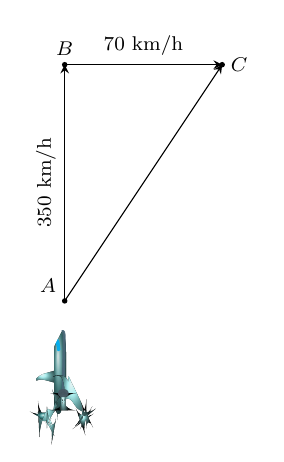
\begin{tikzpicture}[scale=1, font=\footnotesize, line join=round, line cap=round, >=stealth]
			\tikzset{
				maybay/.pic={
					\begin{scope}[line width=1pt,opacity=0.95]
						\fill[ball color =cyan!40!gray,,rounded corners=2mm](-5.6,3)--++(60:0.8)--++(2:0.55)--++(-90:2)--cycle;
						%Hai cánh
						\fill[ball color =cyan!90!gray!40!white](-0.4,1.5)..controls++(75:2)and++(-68:0.75)..(-0.15,4)--++(-5:0.35)..controls++(-50:0.95)and++(106:2)..(1.25,1.5)--cycle;
						%Thân
						\fill[ball color =cyan!30!gray](-4.85,1)..controls++(-90:0.6) and++(180:0.2)..(-4,0.5)--++(-12:3.3)--++(0:4)..controls++(0:2) and++(-172:1)..(6,0)..controls++(8:1)and++(-90:0.1)..(6.85,0.3)..controls++(90:0.2) and++(-30:1)..(5,1.3)..controls++(90:0.25) and++(0:8)..(-4,1.5)--cycle;
						\draw[cyan!40!black](6.85,0.3)..controls++(-90:0.5) and++(0:6)..(-2,0.2);
						% Cánh phải
						\fill[ball color =cyan!90!gray!40!white,rounded corners=2mm](-1.8,0)--++(-5:0.35)--++(-147:4.85)--++(-50:0.7)--++(25.5:6.5)..controls++(-155.5:0.5) and++(-170:0.15)..(1.5,-0.25)..controls++(120:0.5) and++(2:1)..(-1.8,0);
						\fill[ball color =cyan!90!gray!40!white,rounded corners=2mm](-6.1,-2.3)--++(-54:0.7)--++(-28:0.7)--++(25.5:.35)--++(-180:.2)--++(135:1.2)--cycle;
						%Thân đuôi
						\fill[ball color =cyan!90!gray!40!white,rounded corners=2mm](-6.9,3.6)--++(2:1)..controls++(-35:2) and++(178:2.3)..(-2,1.5)..controls++(-90:0.2) and++(20:1)..(-3.5,1)--++(180:1.2)--cycle;
						%Đuôi
						\fill[ball color =cyan!90!gray!40!white,rounded corners=2mm](-6,2.5)--++(0:1.35)--++(-156:2.5)--++(170:0.75)--cycle;
						\fill[ball color =cyan!70!gray!40!white,rounded corners=2mm](-1.9,-0.17)--++(90:0.72)--++(181:2.45)--++(-90:0.6)--cycle;
						\fill[ball color =cyan!90!gray!10!black,line width=2pt,draw=cyan!30!black,rounded corners=0.5mm](-1.9,-0.18)arc(-90:270:0.2 and 0.38);
						\fill[cyan](5.05,1.3)--++(-25:0.8)..controls++(-140:0.55)and++(10:0.5)..(4.2,0.6)..controls++(180:0.15) and++(182:0.45)..(4.3,1.1)..controls++(2:0.5) and++(-135:0.2)..(5.1,1.3);
					\end{scope}
				}
			}
			\path (0,0) coordinate (O) pic[rotate=90,scale=.1]{maybay} 
			(O)+(90:1) coordinate (A)
			++(90:4) coordinate (B)
			++(0:2) coordinate (C)
			;
			\path[fill=black] (A) circle(1pt) node[above left]{$A$}
			(B) circle (1pt) node[above] {$B$}
			(C) circle (1pt) node[right]{$C$}
			;
			\draw[->] (A)--(B) node [midway,above,sloped] {$350$ km/h};
			\draw[->] (B)--(C) node [midway,above,sloped] {$70$ km/h};
			\draw[->] (A)--(C);
	\end{tikzpicture}}
\loigiai{
Ta có $\overrightarrow{AB}+\overrightarrow{BC}=\overrightarrow{AC}$.\\
Do đó độ dài của véc-tơ tổng chính là độ dài véc-tơ $\overrightarrow{AC}$.\\
Tam giác $ABC$ vuông tại $B$, theo định lý Py-ta-go ra có $AC=\sqrt{AB^2+BC^2}=\sqrt{350^2+70^2}=70\sqrt{26}$.\\
Vậy độ dài véc-tơ tổng cần tìm là $70\sqrt{26}$ km/h.}
\end{bt}

% từ: cau-hoi/lop10/0H5_Vecto_chua_xet_toa_do/0H5-4-7_Toan_thuc_te_ap_dung_tich_vo_huong.tex
\begin{bt}%[0H5V4-7]%[Dự Án Đề Kiểm Tra HKI NH22-23-Trương Đăng Khoa]%[THPT Gò Vấp]%Câu 10%[ma:e4a63698]
	Một người dùng một lực $\overrightarrow{F}$ tạo với mặt đất một góc $45^\circ$ và có độ lớn là $20$ $\mathrm{N}$ để kéo một vật dịch chuyển theo đường thẳng một đoạn $80\,\mathrm{m}$. Tính công sinh bởi lực $\overrightarrow{F}$.
	\begin{center}
		\begin{tikzpicture}[scale=1,font=\footnotesize,line join=round,line cap=round,>=stealth]
			\coordinate (A) at (-3,0.75);
			\coordinate (B) at (-3,-0.75);
			\coordinate (C) at (0,-0.75);
			\coordinate (D) at (0,0.75);
			\coordinate (E) at (0,0);
			\coordinate (F) at (45:2.83);
			\coordinate (G) at (4,0);
			\coordinate [label=below:$80\,\mathrm{m}$] (T) at ($(E)!.5!(G)$);
			\coordinate [label=right:$45^\circ$,yshift=-5pt,xshift=0pt] (U) at ($(E)!.25!(F)$);
			\coordinate [label=above:$\overrightarrow{F}$] (V) at ($(E)!.7!(F)$);
			\draw (-2.3,-1) circle (0.25);
			\draw (-0.7,-1) circle (0.25);
			\draw[->] (E)--(F);
			\draw[->] (E)--(G);
			\draw (A)--(B)--(C)--(D)--(A) (-3.5,-1.25)--(4.5,-1.25);
			\draw pic[draw,angle radius=6mm]{angle=G--E--F};
		\end{tikzpicture}
	\end{center}
	\loigiai{
		Công sinh bởi lực $\overrightarrow{F}$ là $A=\left|F\right|\cdot s\cdot\cos\alpha=20\cdot80\cdot\cos45^\circ=800\sqrt{2}\,\,\mathrm{J}$.}
\end{bt}

% từ: cau-hoi/lop10/0H5_Vecto_chua_xet_toa_do/0H5-4-7_Toan_thuc_te_ap_dung_tich_vo_huong.tex
\begin{bt}%[0H5H4-7]%[Dự án đề kiểm tra HKI NH22-23 - Quan Ón]%[Trường Chinh - Đề 3]%[ma:cc50ad65]
	\begin{listEX}
		\item Trong Vật lí, tích vô hướng của $\overrightarrow{F}$ và $\overrightarrow{d}$ biểu diễn công $A$ sinh bởi lực $\overrightarrow{F}$ khi thực hiện độ dịch chuyển $\overrightarrow{d}$. Một người dùng một lực $\overrightarrow{F}$ có cường độ $15 \mathrm{~N}$ kéo một chiếc xe đi quãng đường dài $30 \mathrm{~m}$. Tính công sinh bởi lực $\overrightarrow{F}$, biết rằng góc giữa vecto $\overrightarrow{F}$ và hướng di chuyển là $30^{\circ}$. \dapso{$225\sqrt{3}$ J.}
		\item 
		\immini{
			Để đo khoảng cách từ vị trí $A$ đến vị trí $B$ ở hai bên bờ hồ, bạn An đi dọc bờ hồ từ vị trí $A$ đến vị trí $C$ và tiến hành đo các góc $BAC$ và $BCA$. Biết $AC=25$ m, $\widehat{BAC}=58{,}95^{\circ}$, $\widehat{BCA}=83{,}15^{\circ}$ ( tham khảo hình bên). Hỏi, khoảng cách từ vị trí $A$ đến vị trí $B$ là bao nhiêu mét? \dapso{$40{,}41$ m.}
		}{
			\begin{tikzpicture}[scale=1,font=\footnotesize,line cap=round,line join=round,>=stealth]
				\def\a{3.75}
				\path (0:0) coordinate(A) (58.95:1) coordinate(a) (0:\a) coordinate(C)  + (96.85:1) coordinate(c)  (intersection of A--a and C--c) coordinate(B);
				\fill[cyan!60] (-.5,2) .. controls +(-70:2) and +(150:1) .. (2.5,1) .. controls +(-15:2) and +(-30:1) .. (4.5,3.5) .. controls +(150:1) and +(40:1) .. (2,4) .. controls +(-150:1.5) and +(100:2) .. cycle;
				\draw (A)--(B)--(C)--cycle;
				\foreach \d/\g in {A/-135, B/90, C/-45}
				\fill (\d) circle(1pt) node[shift={(\g:.3)}]{$\d$};
				\path (A)--(C) node[midway,below]{$25$ m} pic[draw,angle radius=.3cm]{angle=C--A--B} (A) node[shift={(20:.8)}]{$58,95^\circ$} pic[draw,angle radius=.3cm]{angle=B--C--A} pic[draw,angle radius=.35cm]{angle=B--C--A} (C) node[shift={(150:.7)}]{$83,15^\circ$};			
			\end{tikzpicture}
		}
		\item Một người bán nước giải khát đang có $48$ g bột cam, 18 l nước và $420$ g đường để pha chế hai loại nước cam $A$ và $B$. Để pha chế $1$ l nước cam loại $A$ cần $30$ g đường, $1$ l nước và $1$ g bột cam, để pha chế $1$ l nước cam loai $B$ cần $10$ g đường $1$ l nước và $4$ g bột cam. Mỗi lít nước cam loại $A$ bán được $30$ nghìn đồng, mỗi lít nước cam loại $B$ bán đựợc $40$ nghìn đồng. Người đó nên pha chế bao nhiêu lít nước cam mỗi loại để có doanh thu cao nhất? \dapso{$8$ lít loại $A$ và $10$ lít loại $B$.}
	\end{listEX}
    \loigiai{
    \begin{enumerate}
    	\item Công sinh bởi lực $\overrightarrow{F}$ là
    	$$ \overrightarrow{F}\cdot \overrightarrow{d} = \left|\overrightarrow{F} \right|\cdot \left|\overrightarrow{d} \right|\cdot \cos 30^\circ = 15\cdot 30\cdot \dfrac{\sqrt{3}}{2} = 225\sqrt{3} \quad \textrm{(J).}$$
    	\item Xét tam giác $ABC$, ta có 
    	$$\widehat{ABC} = 180^\circ - \left( \widehat{BAC} + \widehat{BCA}\right) = 180^\circ - \left( 58{,}95^\circ + 83{,}15^\circ \right) = 37{,}9^\circ.$$
    	Áp dụng định lí hàm sin trong tam giác $ABC$, ta có
    	$$ \dfrac{AC}{\sin\widehat{ABC}} = \dfrac{AB}{\sin\widehat{BCA}} \Rightarrow AB = \dfrac{AC\cdot \sin\widehat{BCA}}{\sin\widehat{ABC}} = \dfrac{25\cdot\sin 83{,}15^\circ}{\sin 37{,}9^\circ} \approx 40{,}41 \quad\textrm{ (m).}$$
    	Vậy khoảng cách từ vị trí $A$ đến vị trí $B$ gần bằng $40{,}41$ mét.
    	\item Gọi $x$ và $y$ (lít) lần lượt là số lít nước cam loại $A$ và loại $B$ cần pha $(x,y \geq 0)$. $\hfill (1)$\\
    	Số gam bột cam cần để pha được $x$ lít nước cam loại $A$ và $y$ lít nước cam loại $B$ là $x + 4y$. Mà người này chỉ có $48$ gam bột cam nên $x + 4y \leq 48$. $\hfill(2)$\\
    	Số lít nước cần để pha được $x$ lít nước cam loại $A$ và $y$ lít nước cam loại $B$ là $x + y$. Mà người này chỉ có $18$ lít nước nên $x + y \leq 18$. $\hfill(3)$\\
    	Số gam đường cần để pha được $x$ lít nước cam loại $A$ và $y$ lít nước cam loại $B$ là $30x + 10y$. Mà người này chỉ có $420$ gam đường nên $30x + 10y \leq 420$. $\hfill(4)$\\
    	Từ $(1)$, $(2)$, $(3)$, $(4)$ ta có hệ bất phương trình
    	$$ \heva{&x \geq 0\\&y \geq 0\\&x + 4y \leq 48\\&x + y \leq 18\\&30x + 10y \leq 420.} \quad (*) $$
    	Vì mỗi lít nước cam loại $A$ bán được $30$ nghìn đồng, mỗi lít nước cam loại $B$ bán đựợc $40$ nghìn đồng nên doanh thu khi bán được $x$ lít nước loại $A$ và $y$ lít nước loại $B$ là $T(x;y) = 30x + 40y$ (nghìn đồng).\\
    	Biểu diễn miền nghiệm của hệ bất phương trình $(*)$ (là phần bị gạch chéo có tính cả các đường biên) như sau.
    	\begin{center}
    		\begin{tikzpicture}[>=stealth,line join=round,line cap=round,font=\footnotesize,scale=1]
    			\draw[->,line width = 1pt] (-0.5,0)--(0,0) node[below left]{$O$}--(5.5,0) node[below]{$x$};
    			\draw[->,line width = 1pt] (0,-0.5) --(0,5) node[right]{$y$};
    			\fill (0,1.2) node[left,scale = 0.7]{$12$} circle (1pt);
    			\fill (0,1.8) node[left,scale = 0.7]{$18$} circle (1pt);
    			\fill (0,4.2) node[left,scale = 0.7]{$42$} circle (1pt);
    			\fill (1.4,0) node[below,scale = 0.7]{$14$} circle (1pt);
    			\fill (1.8,0) node[below,scale = 0.7]{$18$} circle (1pt);
    			\fill (4.8,0) node[below,scale = 0.7]{$48$} circle (1pt);
    			\fill (1.2,0.6) circle (1pt);
    			\fill (0.8,1) circle (1pt);
    			\draw (0,1.2)--(4.8,0) (0,1.8)--(1.8,0) (0,4.2)--(1.4,0);
    			\fill[opacity=.2,pattern= vertical lines] (0,0)--(0,1.2)--(0.8,1)--(1.2,0.6)--(1.4,0)--cycle;
    		\end{tikzpicture}
    	\end{center}
    	Miền nghiệm của hệ $(*)$ là một đa giác có các đỉnh có tọa độ là $(0;0)$, $(0;12)$, $(8;10)$, $(12;6)$, $(14;0)$. Tính toán $T(x;y)$ tại các đỉnh này ta có $T(8;10) = 640$ (nghìn đồng) là lớn nhất.\\
    	Vậy người này cần pha $8$ lít nước cam loại $A$ và $10$ lít nước cam loại $B$ để có doanh thu cao nhất.
    \end{enumerate}
}
\end{bt}

% từ: cau-hoi/lop10/0H9_Phuong_phap_toa_do_trong_mat_phang/0H9-5-0_Bai_toan_tong_hop_thuc_te_PP_toa_do_hoa_3_duo.tex
\begin{bt}%[0H9H5-0]%[Tex hóa SGK CD-CT,T7/22, Ninh Tiến Nam]%[ma:cf804107]
	Gọi tên các đường conic sau
	\begin{center}
		
		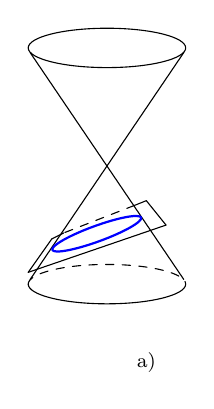
\begin{tikzpicture}[>=stealth,line join=round,line cap=round,font=\footnotesize,scale=.5]
			\draw[black] (-3,3) ellipse (2 and 0.5);
			\draw[black] (-5,-3) arc (-180:0: {2} and 0.5);
			\draw[black,dashed] (-5,-3) arc (180:0: {2} and 0.5);
			\draw (-4.95,2.88) -- (-1.05,-2.88);
			\draw (-4.95,-2.88) -- (-1.05,2.88);
			
			
			
			
			\draw[rotate around={20:(-3.26,-1.72)}, blue, thick] (-3.26,-1.72) ellipse (1.2 and 0.2);
			\draw (-5,-2.7) -- (-1.5,-1.5);
			\draw (-5,-2.7) -- (-4.4,-1.85);
			\draw (-4.4,-1.85) -- (-4.1,-1.7);
			\draw (-1.5,-1.5) -- (-2,-0.88);
			\draw (-2,-0.88) -- (-2.3,-1);
			\draw[dashed] (-2.3,-1) -- (-4.1,-1.7);
			\node at (-2,-5) {a)};
			
			
		\end{tikzpicture}\hspace*{1cm}
		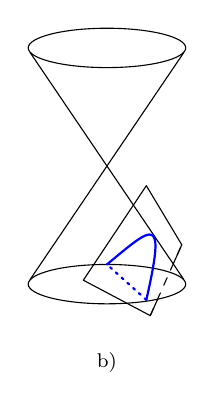
\begin{tikzpicture}[>=stealth,line join=round,line cap=round,font=\footnotesize,scale=.5,rotate =-180]
			\draw[black] (-3,3) ellipse (2 and 0.5);
			\draw[black] (-3,-3) ellipse (2 and 0.5);
			\draw (-4.95,2.88) -- (-1.05,-2.88);
			\draw (-4.95,-2.88) -- (-1.05,2.88);
			
			
			
			
			
			
			\draw[blue, thick] (-4,3.4) .. controls (-4.5,1.2) and (-4.2,1.5) .. (-3,2.5);
			\draw[dotted, blue, thick] (-4,3.4) -- (-3,2.5);
			\draw (-2.4,2.9) -- (-4,0.5);
			\draw (-2.4,2.9) -- (-4.1,3.8) coordinate (A);
			\draw (-4,0.5) -- (-4.9,2) coordinate (B);
			\draw[dashed] (A) -- (B);
			\draw (A) -- (-4.28,3.4);
			\draw (B) -- (-4.7,2.45);
			\node at (-3,5) {b)};
			
			
		\end{tikzpicture}\hspace*{1cm}
		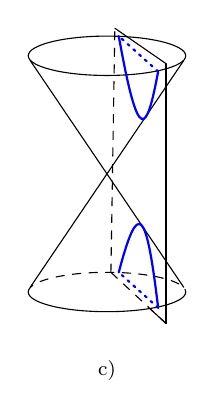
\begin{tikzpicture}[>=stealth,line join=round,line cap=round,font=\footnotesize,scale=.5]
			\draw[black] (3,3) ellipse (2 and 0.5);
			\draw[black] (1,-3) arc (-180:0: {2} and 0.5);
			\draw[black,dashed] (1,-3) arc (180:0: {2} and 0.5);
			
			\draw (4.95,2.88) -- (1.05,-2.88);
			\draw (4.95,-2.88) -- (1.05,2.88);
			
			
			
			\draw (4.5,-3.8) coordinate (A) -- (4.5,2.8) coordinate (B);
			\draw[dashed] (A) -- (3.1,-2.5) coordinate (C);
			\draw (B) -- (3.2,3.7) coordinate (D);
			\draw[dashed] (C) -- (D);
			\draw[blue, thick] (4.3,-3.4) coordinate (E) .. controls (4,-0.9) and (3.8,-0.6) .. (3.3,-2.5) coordinate (F);
			\draw[dotted, blue, thick] (E) -- (F); 
			\draw[blue, thick] (4.3,2.6) coordinate (G) .. controls (4,1) and (3.8,0.7) .. (3.3,3.5) coordinate (H);
			\draw[dotted, blue, thick] (G) -- (H); 
			\draw (A) -- (4.1,-3.43);
			\node at (3,-5) {c)};
		\end{tikzpicture}
	\end{center}
	\loigiai{\begin{itemize}
			\item Hình $a$ là đường tròn.
			\item Hình $b$ là đường parabol.
			\item Hình $c$ là đường hypebol.
		\end{itemize}
	}
\end{bt}

% từ: cau-hoi/lop10/0H9_Phuong_phap_toa_do_trong_mat_phang/0H9-5-0_Bai_toan_tong_hop_thuc_te_PP_toa_do_hoa_3_duo.tex
\begin{bt}%[0H9V5-0]%Câu 3%[ma:7b0cca6a]
	\immini
	{
		Một chiếc đèn có mặt cắt ngang là hình parabol $y^2=2px\ (p>0)$ như hình vẽ. Trong đó chiều rộng hai mép vành là $AB=40$ cm, chiều sâu $h=20$ cm (khoảng cách từ $O$ đến $AB$), bóng đèn nằm ở tiêu điểm $S$. Tìm giá trị của tham số tiêu.
		\shortans{$10$}
	}
	{
		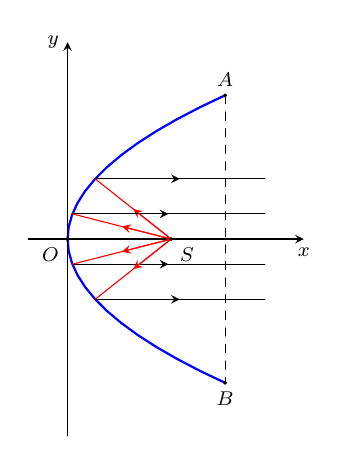
\begin{tikzpicture}[scale=0.5, font=\footnotesize, line join=round, line cap=round, >=stealth]
			
			\draw[domain=-3.65:3.65, blue,thick] plot({3/10*(\x)^2},\x);
			%\draw[gray!10] (-1,-1) grid (5,5);
			\draw[->] (-1,0)--(6,0) node[below]{$x$};
			\draw[->] (0,-5)--(0,5) node[left]{$y$};
			\coordinate (A) at (4,3.65); 
			\coordinate (B) at (4,-3.65); 
			\coordinate (O) at (0,0); 
			\coordinate (C) at (0.12,0.64); 
			\coordinate (C') at (0.12,-0.64); 
			\coordinate (D) at (0.7,1.53); 
			\coordinate (D') at (0.7,-1.53); 
			\coordinate (F) at (5.01,1.53); 
			\coordinate (F') at (5.01,-1.53); 
			\coordinate (G) at (5.01,0.64); 
			\coordinate (G') at (5.01,-0.64); 
			\coordinate (E) at (2.63,0); 
			\coordinate (H1) at (1.67,0.76); 
			\coordinate (H2) at (1.67,-0.76); 
			\coordinate (H3) at (1.38,0.32); 
			\coordinate (H4) at (1.38,-0.32); 
			\coordinate (K1) at (2.85,1.53); 
			\coordinate (K2) at (2.85,-1.53); 
			\coordinate (K3) at (2.56,0.64); 
			\coordinate (K4) at (2.56,-0.64); 
			\draw  (F)--(D) (G)--(C) (F')--(D') (G')--(C') ;
			\draw[dashed] (A)--(B);
			\draw[red,->] (E)--(H1); 
			\draw[->] (D)--(K1) ;
			\draw[red,->] (E)--(H3); 
			\draw[->] (C)--(K3) ;
			\draw[red,->] (E)--(H4); 
			\draw[->] (C')--(K4) ;
			\draw[red,->] (E)--(H2); 
			\draw[->] (D')--(K2) ;
			
			\draw[red] (E)--(C) (E)--(D) (E)--(C') (E)--(D');
			
			\draw[fill=black] (A) circle (1pt) node [above] {$A$};
			\draw[fill=black] (B) circle (1pt) node [below] {$B$};
			\draw[fill=black] (E) circle (1pt) node [below right] {$S$};
			\draw[fill=black] (O) circle (1pt) node [below left] {$O$};
		\end{tikzpicture}
	}
	\loigiai{
		Từ giả thiết ta có parabol đi qua điểm $A(20;20)$ thay vào phương trình $y^2=2px$ do đó $20^2=2p\cdot 20\Leftrightarrow  p=10$.\\
		Nên giá trị tham số tiêu là $p=10$.}
\end{bt}

% từ: cau-hoi/lop11/1D1_Ham_so_luong_giac_va_phuong_trinh_luong/1D1-1-2_Chuyen_doi_don_vi_do_va_radian.tex
\begin{ex}%[1D1B1-2]%[ma:f9062a7f]
	Hàm số $y=\sin  x$
	 \choice
		{đồng biến trên mỗi khoảng $\left(\dfrac{\pi}{2}+k2\pi;\pi+k2\pi\right)$ và nghịch biến trên mỗi khoảng  $\left(\pi+k2\pi;k2\pi\right)$ với $k\in\mathbb{Z}$}
		{đồng biến trên mỗi khoảng  $\left(-\dfrac{3\pi}{2}+k2\pi;\dfrac{5\pi}{2}+k2\pi\right)$ và nghịch biến trên mỗi khoảng $\left(-\dfrac{\pi}{2}+k2\pi;\dfrac{\pi}{2}+k2\pi\right)$ với $k\in\mathbb{Z}$}
		 {đồng biến trên mỗi khoảng $\left(\dfrac{\pi}{2}+k2\pi;\dfrac{3\pi}{2}+k2\pi\right)$ và nghịch biến trên mỗi khoảng $\left(-\dfrac{\pi}{2}+k2\pi;\dfrac{\pi}{2}+k2\pi\right)$ với $k\in\mathbb{Z}$}
		{\True đồng biến trên mỗi khoảng $\left(-\dfrac{\pi}{2}+k2\pi;\dfrac{\pi}{2}+k2\pi\right)$ và nghịch  biến trên mỗi khoảng $\left(\dfrac{\pi}{2}+k2\pi;\dfrac{3\pi}{2}+k2\pi\right)$ với $k\in\mathbb{Z}$}
	\loigiai{ 
	\immini{ 
		Hàm  số $y=\sin x$ đồng biến trên mỗi khoảng $\left(-\dfrac{\pi}{2}+k2\pi;\dfrac{\pi}{2}+k2\pi\right)$ và nghịch biến trên mỗi khoảng $\left(\dfrac{\pi}{2}+k2\pi;\dfrac{3\pi}{2}+k2\pi\right)$ với $k\in\mathbb{Z}$.}{
		\begin{tikzpicture}[scale=.7,font=\footnotesize,line join=round,line cap=round,>=stealth]
				\def\r{3}  \def\m{3.5}
				\def\f  (#1){(#1)}
				\draw[->] (-\r,0)--(\r+0.5,0) node[below] {$x$}node[above]  {$\cos x$};
				\draw[->] (0,-\r)--(0,\r+0.5) node[below  right] {$y$} node[left]{$\sin x$};
				\draw (0,0)  node [below left] {$O$};
				\foreach \x/\g/\z in {2.5/-45/1,-2.5/-135/-1}\fill[black] (\x,0) circle  (1pt)+(\g:0.4) node{$\z$};
				\foreach  \y/\g/\z in {2.5/135/1,-2.5/-135/-1}\fill[black] (0,\y) circle (1pt)+(\g:0.4) node{$\z$};
				\draw[color=white]  (0,0) circle (\r);
				\draw[-latex] (10:\r)  arc (10:70:\r);
				\draw (2.2,-0.2)  node{$2\pi$}
					(2.3,0.2)  node{$0$}
					(.2,2.1) node{$\tfrac{\pi}{2}$} 
					 (-.2,-2.1) node{$\tfrac{3\pi}{2}$}
					(-2.3,0.2) node{$\pi$}; 
				 \draw[-latex] (-10:\r) arc (-10:-70:\r);
				\draw (0,0)  circle (2.5);
				\draw  (2,3) circle (6pt) node{$+$}
					 (2,-3) circle (6pt) node{$-$};
			\end{tikzpicture}
	}} 
\end{ex}

% từ: cau-hoi/lop11/1D1_Ham_so_luong_giac_va_phuong_trinh_luong/1D1-1-2_Chuyen_doi_don_vi_do_va_radian.tex
\begin{ex}%[1D1B1-2]%[ma:ab81c995]
	Hàm số $ y=\sin x $ nghịch  biến trên khoảng nào dưới đây?
	\choice 
		{$ \left(\dfrac{5\pi}{4};\dfrac{7\pi}{4}\right) $} 
		{$ \True \left(\dfrac{3\pi}{4};\dfrac{5\pi}{4}\right)  $}
		{$  \left(\dfrac{3\pi}{2};\dfrac{7\pi}{4}\right) $}
		 {$ \left(\dfrac{7\pi}{4};\dfrac{9\pi}{4}\right) $}
	 \loigiai{
	Vì hàm số $ y=\sin x $ nghịch biến trên mỗi khoảng $ \left(\dfrac{\pi}{2}+k2\pi;\dfrac{3\pi}{2}+k2\pi\right) $ với $k \in \mathbb {Z}$ nên nhận thấy $  \left(\dfrac{3\pi}{4};\dfrac{5\pi}{4}\right) \subset \left(\dfrac{\pi}{2};\dfrac{3\pi}{2}\right) $, vậy trong khoảng này hàm số $ y=\sin x $ nghịch biến.}
\end{ex}

% từ: cau-hoi/lop11/1D1_Ham_so_luong_giac_va_phuong_trinh_luong/1D1-1-3_So_do_cua_mot_goc_luong_giac.tex
\begin{bt}%[1D1N1-3]%[ma:85cb8d1f]
% nguon: Archive/2024/SP-K10-K11-LyVanHoang_TVN-023/11. C1-LuongGiac-lvhoang_TVN-023/dataC1K11/Bai1-Dang2.tex #1944
[CTST, MĐ1]
	Xác định số đo của các góc lượng giác $(Oa,Ob)$ trong hình sau
	\begin{listEX}[4]
		\item
		\begin{tikzpicture}[>=stealth,line join=round,line cap=round,font=\footnotesize,scale=1]
			\def\r{2.5}
			\path
			(0,0) coordinate (O)
			(\r,0) coordinate (a)
			(0,\r) coordinate (b)
			;
			\pic[draw,angle radius=2mm,angle eccentricity=1.5] {right angle = a--O--b};
			\draw (a)--(O)--(b);
			\draw[->] (0:0.5*\r) arc (0:90:0.5*\r);
			\fill[black] (O) circle (1pt);
			\foreach \l/\g in {a/-90,b/180,O/-135}
			\draw[fill=black] (\l)+(\g:.3) node{$\l$};
		\end{tikzpicture}
		\item
		\begin{tikzpicture}[>=stealth,line join=round,line cap=round,font=\footnotesize,scale=1]
			\def\r{2.5}
			\path
			(0,0) coordinate (O)
			(\r,0) coordinate (a)
			(0,\r) coordinate (b)
			;
			\pic[draw,angle radius=2mm,angle eccentricity=1.5] {right angle = a--O--b};
			\draw (a)--(O)--(b);
			\draw[->,domain=0:450,variable=\t,samples=200,>=latex]
			plot ({0.6*(\t+2*450)*cos(\t)/(2*450)},
			{0.6*(\t+ 2*450)*sin(\t)/(2*450)})
			;
			\fill[black] (O) circle (1pt);
			\foreach \l/\g in {a/-90,b/180,O/-135}
			\draw[fill=black] (\l) +(\g:.3) node{$\l$};
		\end{tikzpicture}
		\item
		\begin{tikzpicture}[>=stealth,line join=round,line cap=round,font=\footnotesize,scale=1]
			\def\r{2.5}
			\path
			(0,0) coordinate (O)
			(\r,0) coordinate (a)
			(0,\r) coordinate (b)
			;
			\pic[draw,angle radius=2mm,angle eccentricity=1.5] {right angle = a--O--b};
			\draw (a)--(O)--(b);
			\draw[->,domain=0:810,variable=\t,samples=200,>=latex]
			plot ({0.6*(\t+2*810)*cos(\t)/(2*810)},
			{0.6*(\t+ 2*810)*sin(\t)/(2*810)})
			;
			\fill[black] (O) circle (1pt);
			\foreach \l/\g in {a/-90,b/180,O/-135}
			\draw[fill=black] (\l) +(\g:.3) node{$\l$};
		\end{tikzpicture}
		\item
		\begin{tikzpicture}[>=stealth,line join=round,line cap=round,font=\footnotesize,scale=1]
			\def\r{2.5}
			\path
			(0,0) coordinate (O)
			(\r,0) coordinate (a)
			(0,\r) coordinate (b)
			;
			\pic[draw,angle radius=2mm,angle eccentricity=1.5] {right angle = a--O--b};
			\draw (a)--(O)--(b);
			\draw[->] (0:0.3*\r) arc (0:-270:0.3*\r);
			\fill[black] (O) circle (1pt);
			\foreach \l/\g in {a/-90,b/180,O/-135}
			\draw[fill=black] (\l) +(\g:.3) node{$\l$};
		\end{tikzpicture}
	\end{listEX}
	\loigiai{
		\begin{listEX}[1]
			\item Số đo của góc lượng giác $(Oa,Ob)$ trong hình vẽ là $90^\circ$.
			\item Số đo của góc lượng giác $(Oa,Ob)$ trong hình vẽ là $90^\circ + 360^\circ = 450^\circ$.
			\item Số đo của góc lượng giác $(Oa,Ob)$ trong hình vẽ là $90^\circ + 2\cdot 360^\circ = 810^\circ$.
			\item Số đo của góc lượng giác $(Oa,Ob)$ trong hình vẽ là $\dfrac{3}{4}\cdot \left(-360^\circ\right)=-270^\circ$.
		\end{listEX}
	}
\end{bt}

% từ: cau-hoi/lop11/1D1_Ham_so_luong_giac_va_phuong_trinh_luong/1D1-1-3_So_do_cua_mot_goc_luong_giac.tex
\begin{bt}%[1D1N1-3]%[ma:d116a620]
% nguon: Archive/2024/TOAN_11_XE/TOAN_11_XE/data4/11C1/KNTT-1.1.tex #1194

	Xác định số đo của các góc lượng giác $(Oa,Ob)$ trong hình sau
	\begin{listEX}[4]
		\item 
		\begin{tikzpicture}[>=stealth,line join=round,line cap=round,font=\footnotesize,scale=0.8]
			\def\r{2.5}
			\path 
			(0,0) coordinate (O)
			(\r,0) coordinate (a)
			(0,\r) coordinate (b)
			;
			\pic[draw,angle radius=2mm,angle eccentricity=1.5] {right angle = a--O--b};
			\draw (a)--(O)--(b);
			\draw[->] (0:0.5*\r) arc (0:90:0.5*\r);
			\fill[black] (O) circle (1pt);
			\foreach \l/\g in {a/-90,b/180,O/-135}
			\draw[fill=black] (\l)+(\g:.3) node{$\l$};
		\end{tikzpicture}
		\item 
		\begin{tikzpicture}[>=stealth,line join=round,line cap=round,font=\footnotesize,scale=0.8]
			\def\r{2.5}
			\path 
			(0,0) coordinate (O)
			(\r,0) coordinate (a)
			(0,\r) coordinate (b)
			;
			\pic[draw,angle radius=2mm,angle eccentricity=1.5] {right angle = a--O--b};
			\draw (a)--(O)--(b);
			\draw[->,domain=0:450,variable=\t,samples=200,>=latex]
			plot ({0.6*(\t+2*450)*cos(\t)/(2*450)},
			{0.6*(\t+ 2*450)*sin(\t)/(2*450)})
			;
			\fill[black] (O) circle (1pt);
			\foreach \l/\g in {a/-90,b/180,O/-135}
			\draw[fill=black] (\l) +(\g:.3) node{$\l$};
		\end{tikzpicture}
		\item 
		\begin{tikzpicture}[>=stealth,line join=round,line cap=round,font=\footnotesize,scale=0.8]
			\def\r{2.5}
			\path 
			(0,0) coordinate (O)
			(\r,0) coordinate (a)
			(0,\r) coordinate (b)
			;
			\pic[draw,angle radius=2mm,angle eccentricity=1.5] {right angle = a--O--b};
			\draw (a)--(O)--(b);
			\draw[->,domain=0:810,variable=\t,samples=200,>=latex]
			plot ({0.6*(\t+2*810)*cos(\t)/(2*810)},
			{0.6*(\t+ 2*810)*sin(\t)/(2*810)})
			;
			\fill[black] (O) circle (1pt);
			\foreach \l/\g in {a/-90,b/180,O/-135}
			\draw[fill=black] (\l) +(\g:.3) node{$\l$};
		\end{tikzpicture}
		\item 
		\begin{tikzpicture}[>=stealth,line join=round,line cap=round,font=\footnotesize,scale=0.8]
			\def\r{2.5}
			\path 
			(0,0) coordinate (O)
			(\r,0) coordinate (a)
			(0,\r) coordinate (b)
			;
			\pic[draw,angle radius=2mm,angle eccentricity=1.5] {right angle = a--O--b};
			\draw (a)--(O)--(b);
			\draw[->] (0:0.3*\r) arc (0:-270:0.3*\r);
			\fill[black] (O) circle (1pt);
			\foreach \l/\g in {a/-90,b/180,O/-135}
			\draw[fill=black] (\l) +(\g:.3) node{$\l$};
		\end{tikzpicture}
	\end{listEX}
	\loigiai{
		\begin{listEX}[1]
			\item Số đo của góc lượng giác $(Oa,Ob)$ trong hình vẽ là $90^\circ$.
			\item Số đo của góc lượng giác $(Oa,Ob)$ trong hình vẽ là $90^\circ + 360^\circ = 450^\circ$.
			\item Số đo của góc lượng giác $(Oa,Ob)$ trong hình vẽ là $90^\circ + 2\cdot 360^\circ = 810^\circ$.
			\item Số đo của góc lượng giác $(Oa,Ob)$ trong hình vẽ là $\dfrac{3}{4}\cdot \left(-360^\circ\right)=-270^\circ$.
		\end{listEX}
	}
\end{bt}

% từ: cau-hoi/lop11/1D1_Ham_so_luong_giac_va_phuong_trinh_luong/1D1-1-4_Do_dai_cua_mot_cung_tron.tex
\begin{ex}%[1D1N1-4]%[ma:2054b4ca]
	Ở góc phần tư  thứ tư của đường tròn lượng giác. hãy chọn kết quả đúng trong các kết quả sau đây.
	\choice 
		{$\tan  \alpha >0$}
		{$\sin \alpha >0$} 
		 {\True $\cos \alpha >0$}
		{$\cot \alpha >0$} 
	 \loigiai{
		Ở góc phần tư thứ tư thì $\sin \alpha <0$, $\cos \alpha >0$,  $\tan \alpha <0$, $\cot \alpha <0$.
	 }
\end{ex}

% từ: cau-hoi/lop11/1D1_Ham_so_luong_giac_va_phuong_trinh_luong/1D1-2-1_Cau_hoi_ly_thuyet.tex
\begin{ex}%[1D1B2-1]%[ma:f4a76535]
	 Giải phương trình $ \cos2x=-\dfrac{1}{2}. $
	\choice 
		{$ x=\pm \dfrac{\pi}{3}+k2\pi, \, \left(k\in \Bbb{Z}\right) $} 
		{$ x=\pm \dfrac{\pi}{6}+k\pi,  \, \left(k\in \Bbb{Z}\right) $}
		{$ x=\pm \dfrac{2\pi}{3}+k2\pi,  \, \left(k\in \Bbb{Z}\right) $}
		{\True $ x=\pm \dfrac{\pi}{3}+k\pi, \, \left(k\in  \Bbb{Z}\right) $}
	\loigiai{ 
		 Ta có: $ \cos2x=-\dfrac{1}{2}\Leftrightarrow \cos2x=\cos\dfrac{2\pi}{3}\Leftrightarrow 2x=\pm \dfrac{2\pi}{3}+k2\pi$
		 $ \Leftrightarrow x\pm \dfrac{\pi}{3}+k\pi $ với $ k\in \Bbb{Z}. $
	} 
\end{ex}

% từ: cau-hoi/lop11/1D1_Ham_so_luong_giac_va_phuong_trinh_luong/1D1-2-2_Xet_dau_gia_tri_luong_giac_Tinh_gia_tri_luong.tex
\begin{ex}%[1D1H2-2]%[ma:a6163f5a]
	Tính giá trị của $\cos \left[\dfrac{\pi  }{3} +(2k+1)\pi \right]$.
	\shortans{-0,5} 
	 \loigiai{
		Ta có $\cos \left[\dfrac{\pi }{3} +(2k+1)\pi \right]=\cos \left(\dfrac{\pi }{3} +\pi +k2\pi \right)=\cos \left(\dfrac{\pi }{3} +\pi \right)=-\cos  \dfrac{\pi }{3} =-\dfrac{1}{2}$.
	} 
\end{ex}

% từ: cau-hoi/lop11/1D1_Ham_so_luong_giac_va_phuong_trinh_luong/1D1-2-3_Bien_doi_rut_gon_bieu_thuc_luong_giac_chung_m.tex
\begin{bt}%[1D1V2-3]%[ma:b55a58d8]
% nguon: Archive/2024/SP-K10-K11-LyVanHoang_TVN-023/11. C1-LuongGiac-lvhoang_TVN-023/dataC1K11/Bai-1-Dang-8-RutGonBieuThucLuongGiac.tex #1819
[SBT KNTT,MĐ3]
	Biết $\sin a+\cos a=m$. Hãy tính theo $m$
	\begin{enumerate}
		\item $\sin a\cos a$;
		\item $\sin^3a+\cos^3a$;
		\item $\sin^4a+\cos^4a$.
	\end{enumerate}
	\loigiai{
		\begin{enumerate}
			\item Ta có $( \sin a+\cos  a)^2=\sin ^2a+2\sin a\cos a+{\cos ^2}a=1+2\sin a\cos a\ (*)$.\\
			Mặt khác $\sin a+\cos a=m$ suy ra $m^2=1+2\sin a\cos a$ hay $\sin a \cos a =\dfrac{m^2-1}{2}$.
			\item $\sin^3a+\cos^3a=(\sin a+\cos a)^3-3\sin a\cos a\left(\sin^2a+\cos^2a\right)=m^3-\dfrac{3}{2}\left(m^2-1\right).$
			\item $\left(\sin^4a+\cos^4a\right)=\left(\sin^2a+\cos^2a\right)^2-2\sin^2a\cos^2a=1-2\left(\dfrac{m^2-1}{2}\right)^2=\dfrac{-m^4+2m^2+1}{2}$.
		\end{enumerate}
	}
\end{bt}

% từ: cau-hoi/lop11/1D1_Ham_so_luong_giac_va_phuong_trinh_luong/1D1-3-1_Cau_hoi_ly_thuyet.tex
\begin{ex}%[1D1N3-1]%[ma:63aac56a]
	Hãy chọn kết quả \textbf{sai} trong các kết quả sau đây 
	\choice 
		 {$\cos (-\alpha)=\cos \alpha $}
		{\True $\sin  (\pi +\alpha)=\sin \alpha $}
		{$\tan (\pi -\alpha)=-\tan \alpha  $}
		{$\cot \left(\dfrac{\pi}{2}  -\alpha \right)=\tan \alpha $}
	 \loigiai{
	Ta có $\sin (\pi +\alpha)=-\sin \alpha $. Do đo $\sin (\pi +\alpha)=\sin \alpha  $ là sai.}
\end{ex}

% từ: cau-hoi/lop11/1D1_Ham_so_luong_giac_va_phuong_trinh_luong/1D1-3-3_Ap_dung_cong_thuc_nhan_doi_ha_bac.tex
\begin{ex}%[1D1H3-3]%[ma:a07a5d9d]
 Cho $\sin\alpha=\dfrac{3}{5}$ và $\cos \alpha=-\dfrac{4}{5}$.  Mỗi khẳng định dưới đây đúng hay sai?
  \choiceTF
  {\True  $\cos2\alpha=\dfrac{7}{25}$}
  {$\sin2\alpha=\dfrac{6}{5}$} 
  {\True  $\tan2\alpha=-\dfrac{24}{7}$}
  {\True  $\cot2\alpha=-\dfrac{7}{24}$}
 \loigiai{ 
  \begin{itemchoice}
    \itemch $\cos2\alpha=1-2\sin^2\alpha=1-2\left(\dfrac{3}{5}\right)^2=\dfrac{7}{25}$.
    \itemch $\sin2\alpha=2\sin\alpha\cos\alpha=2\cdot\dfrac{3}{5}\cdot\left(-\dfrac{4}{5}\right)=-\dfrac{24}{25}$.
   \itemch $\tan2\alpha=\dfrac{\sin2\alpha}{\cos2\alpha}=-\dfrac{24}{25}:\dfrac{7}{25}=-\dfrac{24}{7}.$ 
    \itemch $\cot2\alpha=\dfrac{1}{\tan2\alpha}=-\dfrac{7}{24}.$
  \end{itemchoice}
 } 
\end{ex}

% từ: cau-hoi/lop11/1D1_Ham_so_luong_giac_va_phuong_trinh_luong/1D1-3-4_Ap_dung_cong_thuc_bien_doi_tich_tong.tex
\begin{bt}%[1D1H3-4]%[ma:43d5d269]
% nguon: Archive/2024/SP-K10-K11-LyVanHoang_TVN-023/11. C1-LuongGiac-lvhoang_TVN-023/dataC1K11/Bai2-Dang3-Congthucbiendoitichthanhtong.tex #1782
%[Huỳnh Đức Vũ, dự án bài giảng K10-11]
	Biến đổi thành tổng các biểu thức sau
	\begin{listEX}[2]
		\item $B= \sin 5x\cos 3x$.
		\item $E=\sin (x+y) \cos (x-y)$.
		\item $F=\sin \left( x+30^{\circ}\right) \cos \left( x-30^{\circ}\right)$.
		\end{listEX}
	\loigiai{
		\begin{enumerate}
			\item $B= \sin 5x\cos 3x= \dfrac{1}{2}\left( \sin 2x + \sin 8x\right)$.
			\item $E=\sin (x+y) \cos (x-y)= \dfrac{1}{2}\left( \sin 2y+ \sin 2x\right)$.
			\item $F=\sin \left( x+30^{\circ}\right) \cos \left( x-30^{\circ}\right)= \dfrac{1}{2}\left( \sin 60^\circ + \sin 2x\right)$.
			\end{enumerate}
	}
\end{bt}

% từ: cau-hoi/lop11/1D1_Ham_so_luong_giac_va_phuong_trinh_luong/1D1-3-5_Ket_hop_nhieu_cong_thuc_luong_giac.tex
\begin{ex}%[1D1V3-5]%[ma:fa6d4865]
	Tổng $A=\tan{9^\circ}+\cot{9^\circ}+\tan{15^\circ}+\cot{15^\circ}-\tan{27^\circ}-\cot{27^\circ}$ bằng 
	\choice 
		 {$4$}
		 {$-4$}
		{\True  $8$}
		{$-8$} 
	 \loigiai{
		Ta có 
		\allowdisplaybreaks 
		\begin{align*}
			A&=\tan 9^\circ+\cot 9^\circ+\tan 15^\circ+\cot 15^\circ-\tan  27^\circ-\cot 27^\circ \\
			 &=\tan 9^\circ+\cot 9^\circ-\tan 27^\circ-\cot 27^\circ+\tan 15^\circ+\cot 15^\circ \\
			&=\tan 9^\circ+\tan81^\circ-\tan 27^\circ-\tan63^\circ+\tan 15^\circ+\cot  15^\circ.
		\end{align*}
		 Ta có
		\begin{align*}\tan 9^\circ-\tan 27^\circ+\tan81^\circ-\tan63^\circ&=\dfrac{-\sin 18^\circ}{\cos 9^\circ \cdot\cos 27^\circ}+\dfrac{\sin 18^\circ}{\cos 81^\circ \cdot\cos 63^\circ}\\
			&=\sin  18^\circ\left(\dfrac{\cos 9^\circ \cdot\cos 27^\circ-\cos 81^\circ\cdot \cos 63^\circ}{\cos 81^\circ \cdot \cos 63^\circ \cdot \cos 9^\circ \cdot\cos 27^\circ}\right)\\
			&=\dfrac{\sin 18^\circ\left(\cos 9^\circ \cdot\cos 27^\circ-\sin 9^\circ \cdot\sin 27^\circ\right)}{\cos 81^\circ \cdot\cos 63^\circ \cdot\cos 9^\circ \cdot\cos 27^\circ}\\ &=\dfrac{4\sin 18^\circ \cdot \cos 36^\circ}{\left(\cos 72^\circ+\cos  90^\circ\right)\left(\cos 36^\circ+\cos 90^\circ\right)}\\
			&=\dfrac{4\sin  18^\circ}{\cos 72^\circ}=4.
		\end{align*}\\
		$\tan  15^\circ+\cot 15^\circ=\dfrac{\sin215^\circ+\cos215^\circ}{\sin 15^\circ\cdot \cos 15^\circ}=\dfrac{2}{\sin 30^\circ}=4$.\\
		Vậy $A=8$. 
	} 
\end{ex}

% từ: cau-hoi/lop11/1D1_Ham_so_luong_giac_va_phuong_trinh_luong/1D1-3-5_Ket_hop_nhieu_cong_thuc_luong_giac.tex
\begin{bt}%[1D1N3-5]%[ma:b7ec7bff]
% nguon: Archive/SP_KhoLatex/ID6_old/1K1-2.tex #3591
%[Dự án 1 - TLDH - TeamTeXHoa - Huỳnh Xuân Tín]
	Không dùng máy tính. Hãy tính $\sin 18^{\circ}$.
	\loigiai{
		Vì $54^{\circ}+36^{\circ}=90^{\circ}$ nên $\sin 54^{\circ}=\cos 36^{\circ}$.
		Ta có $\cos 36^{\circ}=\cos \left(2.18^{\circ}\right)=1-2 \sin ^2 18^{\circ}$ và
		$$
		\begin{aligned}
		& \sin 54^{\circ}=\sin \left(18^{\circ}+36^{\circ}\right)=\sin 18^{\circ} \cos 36^{\circ}+\sin 36^{\circ} \cos 18^{\circ} \\
		& =\sin 18^{\circ} \cdot\left(1-2 \sin ^2 18^{\circ}\right)+2 \sin 18^{\circ} \cos ^2 18^{\circ}=\sin 18^{\circ} \cdot\left(1-2 \sin ^2 18^{\circ}\right)+2 \sin 18^{\circ}\left(1-\sin ^2 18^{\circ}\right) \\
		& =3 \sin 18^{\circ}-4 \sin ^3 18^{\circ}.
		\end{aligned}
		$$
		Do đó, đồng nhất thức ta được
		$$
		\begin{aligned}
		& 3 \sin 18^{\circ}-4 \sin ^3 18^{\circ}=1-2 \sin ^2 18^{\circ} \Leftrightarrow\left(\sin 18^{\circ}-1\right)\left(4 \sin ^2 18^{\circ}+2 \sin 18^{\circ}-1\right)=0 \\
		& \Leftrightarrow \sin 18^{\circ}=1 \text { hoặc } \sin 18^{\circ}=\dfrac{\sqrt{5}-1}{2} \text { hoặc } \sin 18^{\circ}=\dfrac{\sqrt{5}+1}{2}.
		\end{aligned}
		$$
		Vì $0<\sin 18^{\circ}<1$ nên $\sin 18^{\circ}=\dfrac{\sqrt{5}-1}{2}$.	
	}	
\end{bt}

% từ: cau-hoi/lop11/1D1_Ham_so_luong_giac_va_phuong_trinh_luong/1D1-4-2_Tim_tap_xac_dinh.tex
\begin{ex}%[1D1H4-2]%[ma:7416fee8]
	Tìm tập  xác định của các hàm số sau đây
	\begin{listEX}[3]
		\item $y=\dfrac{1-\cos x}{\sin  x}$.
		\item  $y=\sqrt{\dfrac{1+\cos x}{2-\cos x}}$.
		\item $y=\tan x$. 
		\item $y=\cot x+\sin 5x+\cos x$. 
		\item $y=\dfrac{\cot  x}{\cos x-1}$.
		\item $y=\cot  x$.
		\item  $y=\dfrac{1-\cos x}{\sin x-1}$.
		\item $y=\tan  x+\cot x$.
		\item $y=\dfrac{\cos  x}{\sin x+1}$.
		 \item $y=\tan \left(2x+\dfrac{\pi}{3} \right)$.
		\item $y=\sin \left(\dfrac{5x}{x^2-1} \right)$. 
		\item $y=\sqrt{2-\sin x}$. 
	\end{listEX}
	 \loigiai{
		\begin{enumerate}
			\item Biểu thức $\dfrac{1-\cos x}{\sin  x}$ có nghĩa khi $\sin x\ne 0$, tức là $x\ne k\pi$, $ k\in \mathbb{Z}$.\\
			Vậy tập xác định của hàm số $y=\dfrac{1-\cos  x}{\sin x}$ là $\mathscr{D}=\mathbb{R}\setminus \left\{k\pi, k\in \mathbb{Z}\right\}$.
			\item Biểu thức $\sqrt{\dfrac{1+\cos x}{2-\cos  x}}$ có nghĩa khi $\heva{&\dfrac{1+\cos x}{2-\cos x} \ge 0\\&2-\cos x\ne 0.}$\\
			Vì $-1\le \cos x\le 1$ nên $1+\cos x\ge 0$ với mọi $x\in \mathbb{R}$ và $2-\cos x\ge  1> 0$ với mọi $x\in \mathbb{R}$.\\
			Do đó  $2-\cos x\ne 0$ với mọi $x\in \mathbb{R}$ và $\dfrac{1+\cos x}{2-\cos x} \ge 0$ với mọi $x\in \mathbb{R}$.\\
			Vậy tập xác định của hàm  số $y=\sqrt{\dfrac{1+\cos x}{2-\cos x}}$ là $\mathscr{D}=\mathbb{R}$.
			\item Điều kiện xác định  $\cos x\ne 0\Leftrightarrow x\ne \dfrac{\pi}{2}+k\pi$, $k\in \mathbb{Z}$. \\
			Vậy tập xác định $\mathscr{D}=\mathbb{R} \setminus \left\{\dfrac{\pi}{2}+k\pi, k\in \mathbb{Z}\right\}$. 
			\item Hàm số xác  định khi $\sin x\ne 0\Leftrightarrow x\ne k\pi$, $k\in \mathbb{Z}$. \\
			Vậy $\mathscr{D}=\mathbb{R} \setminus \left\{k\pi, k\in \mathbb{Z}\right\}$. 
			\item Điều kiện xác định của hàm số là $\heva{&\sin x\ne 0\\&\cos x\ne 1}\Leftrightarrow \heva{&x\ne k\pi\\&x\ne l2\pi} \left(k,l\in {\bf \mathbb{Z}}\right)$ $\Rightarrow  x\ne k\pi$, $ k\in \mathbb{Z}$.\\
			Vậy tập xác định của hàm số $y=\dfrac{\cot x}{\cos  x-1}$ là $\mathscr{D}=\mathbb{R}\setminus \left\{k\pi, k\in {\bf \mathbb{Z}}\right\}$.
			\item Điều kiện  $\sin x\ne 0\Leftrightarrow x\ne k\pi$, $ k\in \mathbb{Z}$. \\
			Vậy tập xác định của hàm số là $\mathscr{D}=\mathbb{R}\setminus  \left\{k\pi, k\in\mathbb{Z}\right\}$.
			 \item Điều kiện xác định của hàm số là $\sin x-1\ne 0$ $\Leftrightarrow \sin x\ne 1$ $\Leftrightarrow x\ne \dfrac{\pi}{2}+k2\pi,\; \left(k\in \mathbb{Z}\right)$.\\
			Vậy tập xác  định của hàm số là $\mathbb{R}\setminus \left\{\dfrac{\pi}{2}+k2\pi \right\}$.
			\item Điều kiện $\sin x\cdot\cos  x\ne 0\Leftrightarrow \sin 2x\ne 0\Leftrightarrow 2x\ne k\pi \Leftrightarrow x\ne \dfrac{k\pi}{2}$, $\left(k\in \mathbb{Z}\right)$.
			\item Điều kiện $\sin x+1\neq 0\Leftrightarrow \sin x\neq -1\Leftrightarrow x\neq-\dfrac{\pi}{2}+k2\pi,\;  \left(k\in \mathbb{Z}\right)$.\\
			Vậy  tập xác định $\mathscr{D}=\mathbb{R}\setminus\left\{-\dfrac{\pi}{2}+k2\pi\mid k\in \mathbb{Z}\right\}$.
			\item Hàm số $y=\tan \left(2x+\dfrac{\pi}{3} \right)$ xác định khi và chỉ khi 
			\[\cos \left(2x+\dfrac{\pi}{3} \right)\ne  0\Leftrightarrow 2x+\dfrac{\pi}{3} \ne \dfrac{\pi}{2}+k\pi \Leftrightarrow x\ne \dfrac{\pi}{12}+k\dfrac{\pi}{2},\; \left(k\in \mathbb{Z}\right).
			 \]
			\item Hàm số $y=\sin \left(\dfrac{5x}{x^2-1} \right)$ xác định $\Leftrightarrow x^2-1\ne 0\Leftrightarrow  x\ne \pm 1$. \\
			Vậy $\mathscr{D}=\mathbb{R}\setminus  \left\{\pm 1\right\}$.
			\item Ta có $-1\le \sin  x\le 1\Rightarrow 2-\sin x > 0$. \\
			Do đó, hàm só luôn luôn xác định  hay $\mathscr{D}=\mathbb{R}$.
		\end{enumerate}
	} 
\end{ex}

% từ: cau-hoi/lop11/1D1_Ham_so_luong_giac_va_phuong_trinh_luong/1D1-4-6_Tim_tap_gia_tri_va_min_max.tex
\begin{bt}%[1D1H4-6]%[ma:a4f23363]
% nguon: Archive/SP_KhoLatex/ID6_old/1K1-3.tex #3543
%[Dự án 1 - TLDH - TeamTeXHoa - Lê Minh Cường]
	Tìm giá trị lớn nhất, giá trị nhỏ nhất của hàm số:
	\begin{listEX}[2]
		\item $y=2 \sin \left(x+\dfrac{\pi}{4}\right)+1$
		\item $y=2 \sqrt{\cos x+1}-3$
	\end{listEX}
	\loigiai{
		\begin{listEX}[1]
			\item  Ta có
			\begin{center}
				$-1 \leq \sin \left(x+\dfrac{\pi}{4}\right) \leq 1 \Rightarrow -2 \leq 2 \sin \left(x+\dfrac{\pi}{4}\right) \leq 2 \Rightarrow -1 \leq 2 \sin \left(x+\dfrac{\pi}{4}\right)+1 \leq 3$.
			\end{center}
			Hay $-1 \leq y \leq 3$. Suy ra\\
			$\max y =3$ khi $\sin \left(x+\dfrac{\pi}{4}\right)=1 \Leftrightarrow x=\dfrac{\pi}{4}+k2 \pi$, $k \in \mathbb{Z}$.\\
			$\min y =-1$ khi $\sin \left(x+\dfrac{\pi}{4}\right)=-1 \Leftrightarrow x=-\dfrac{3\pi}{4}+k2 \pi$, $k \in \mathbb{Z}$.
			\item  Ta có
			\begin{eqnarray*}
				& & -1 \leq \cos x \leq 1\\
				&\Rightarrow & 0 \leq \cos x+1 \leq 2\\
				&\Rightarrow & 0 \leq \sqrt{\cos x+1} \leq \sqrt{2}\\
				&\Rightarrow & 0 \leq 2 \sqrt{\cos x+1} \leq 2 \sqrt{2}\\
				&\Rightarrow & -3 \leq 2 \sqrt{\cos x+1}-3 \leq 2 \sqrt{2}-3
			\end{eqnarray*}
			Hay $-3 \leq y \leq 2 \sqrt{2}-3$. Suy ra\\
			$\max y=2 \sqrt{2}-3$ khi $\cos x=1 \Leftrightarrow x=k2 \pi$, $k \in \mathbb{Z}$.\\		
			$\min y=-3$ khi $\cos x=0 \Leftrightarrow x=\dfrac{\pi}{2}+k\pi$, $k \in \mathbb{Z}$.
		\end{listEX}
	}
\end{bt}

% từ: cau-hoi/lop11/1D1_Ham_so_luong_giac_va_phuong_trinh_luong/1D1-4-7_Bang_bien_thien_va_do_thi.tex
\begin{ex}%[1D1H4-7]%[ma:a09c1088]
	Cho đồ thị hàm số $f\left( x \right)$ như hình vẽ dưới đây. Hỏi tịnh tiến đồ thị hàm số $f\left( x \right)$ theo vectơ $\overrightarrow{v}=\left( \dfrac{\pi }{2};0 \right)$ thì được đồ thị hàm số 
	\begin{center}
		\begin{tikzpicture}[>=stealth,line join=round,line cap=round,font=\footnotesize,scale=0.8]
				\draw[->] (-6,0) -- (6.5,0) node[below] {\small  $x$};
				\draw[->] (0,-1.8) -- (0,2) node[right]  {\small $y$};
				\draw[samples=100,domain=-6:6] plot (\x,{cos ((\x)*180/pi)}); 
				\draw (0,0) node [below left] {$O$}; 
				\draw (0,1) node [above  left] {$1$};
				\draw (0,-1) node [below left]  {$-1$};
				\draw (-4.71,0) node[above] {$-\frac{3\pi}{2}$}; 
				\draw (4.71,0) node[above] {$\frac{3\pi}{2}$}; 
				\draw (-3.17,0) node[above]  {$-\pi$};
				 \draw (pi,0) node[above] {$\pi$};
				\draw[dashed] (-1.57,0)  node[below] {$-\frac{\pi}{2}$};
				\draw[dashed] (1.57,0)  node[below] {$\frac{\pi}{2}$};
				 \draw[dashed] (pi,0)--(pi,-1);
				\draw[dashed]  (-pi,0)--(-pi,-1);
			\end{tikzpicture}
	\end{center}
	 \choice
		{$y=\tan x$} 
		{\True $y=\sin x$} 
		 {$y=\cos x$}
		{$y=\cot x$} 
	\loigiai{ 
	Theo hình vẽ thì đồ thị trong hình là của hàm số $y=\cos x$. Khi tịnh tiến theo vectơ $\overrightarrow{v}=\left( \dfrac{\pi }{2};0  \right)$ thì ta được đồ thị của hàm số $y=\cos \left( x-\dfrac{\pi }{2} \right)=\sin x$.}
\end{ex}

% từ: cau-hoi/lop11/1D1_Ham_so_luong_giac_va_phuong_trinh_luong/1D1-4-7_Bang_bien_thien_va_do_thi.tex
\begin{ex}%[1D1H4-7]%[ma:468c35b5]
 Cho hàm số $y=\tan x$. Xét tính đúng-sai  của các phát biểu sau:
  \choiceTF
  {$y=\tan x$ là hàm  số lẻ, đồ thị đối xứng qua trục tung}
  {\True Đồ thị hàm số $y=\tan x$ có dạng\\ 
  \begin{center}
  \begin{tikzpicture}[line join=round,line cap=round,>=stealth,scale=.95,transform shape]
     \pgfmathsetmacro{\xmin}{-1.5*pi}
    \pgfmathsetmacro{\xmax}{1.5*pi} 
    \def\ymin{-3} \def\ymax{3}  \def\rt{.03}
     \draw[->](\xmin-.1,0)--(\xmax+1,0) node[below]{$x$};
    \draw[->](0,\ymin)--(0,\ymax+.5) node[left]{$y$}; 
    \draw (0,0)  node[below right]{$O$};
    \foreach \i in {-1,0,1}{ 
     \pgfmathsetmacro{\batdau}{\i*pi-1.25} 
     \pgfmathsetmacro{\left}{(\i-0.5)*pi} 
     \pgfmathsetmacro{\ketthuc}{\i*pi+1.25} 
      \draw[dashed,thin] (\left,\ymin)--(\left,\ymax);
     \draw[domain=\batdau:\ketthuc,samples=100,smooth,semithick]  plot (\x,{tan (\x r)});
     }
    \draw[dashed,thin] (1.5*pi,\ymin)--(1.5  * pi,\ymax);
    \draw[dash  pattern=on 2pt off 1.5pt,thin]
      (-pi,0) node[above]{-$\pi$}
     (pi,0) node[above]{$\pi$}; 
   \end{tikzpicture}
  \end{center}
  } 
  {Đồ thị hàm số $y=\tan  x$ cắt trục hoành tại 3 điểm có hoành độ trong $\left(0;2\pi \right)$}
  {$x=2$  là hoành độ giao điểm của hai đồ thị $y=\tan x$ và $y=2\tan x+\sqrt{3}$}
 \loigiai{ 
  \begin{itemchoice}
   \itemch $y=\tan x$ là hàm  số lẻ, đồ thị đối xứng qua gốc toạ độ
   \itemch  $y=\tan x$ đồ thị có dạng sau:
   \begin{center}
    \begin{tikzpicture}[line join=round,line cap=round,>=stealth,scale=.95,transform shape]
       \pgfmathsetmacro{\xmin}{-1.5*pi}
      \pgfmathsetmacro{\xmax}{1.5*pi} 
      \def\ymin{-3} \def\ymax{3} \def\rt{.03} 
      \draw[->](\xmin-.1,0)--(\xmax+1,0) node[below]{$x$}; 
      \draw[->](0,\ymin)--(0,\ymax+.5) node[left]{$y$}; 
      \draw (0,0)  node[below right]{$O$};
       \foreach \i in {-1,0,1}{
      \pgfmathsetmacro{\batdau}{\i*pi-1.25} 
      \pgfmathsetmacro{\left}{(\i-0.5)*pi} 
       \pgfmathsetmacro{\ketthuc}{\i*pi+1.25}
      \draw[dashed,thin]  (\left,\ymin)--(\left,\ymax);
      \draw[domain=\batdau:\ketthuc,samples=100,smooth,semithick] plot (\x,{tan  (\x r)});
       }
      \draw[dashed,thin] (1.5*pi,\ymin)--(1.5 *  pi,\ymax);
      \draw[dash pattern=on  2pt off 1.5pt,thin]
       (-pi,0) node[above]{-$\pi$}
      (pi,0) node[above]{$\pi$}; 
     \end{tikzpicture}
   \end{center}
   \itemch Đồ thị hàm số $y=\tan x$  cắt trục hoành tại 3 điểm có hoành độ trong $\left(0;2\pi \right)$.\\
   Xét phương  trình hoành độ giao điểm $\tan x=0\Leftrightarrow x=k\pi \left(k\in \mathbb{Z}\right)$.\\
   Trong khoảng $\left(0;2\pi  \right)$ ta có một nghiệm là $x=\pi$.
   \itemch $x=2$ là hoành độ  giao điểm của hai đồ thị $y=\tan x$ và $y=2\tan x+\sqrt{3}$.\\
   Phương trình hoành  độ giao điểm đồ thị hàm số $y=\tan x$ và $y=2\tan x+\sqrt{3}$ là
   \allowdisplaybreaks 
   \begin{eqnarray*}
    &&\tan x=2\tan x+\sqrt{3} \\ 
    &\Leftrightarrow& \tan x=\sqrt{3} \\ 
    &\Leftrightarrow& \tan x=\tan  \dfrac{\pi}{3}\\
    &\Leftrightarrow& x=\dfrac{\pi}{3}+k\pi \left(k\in  \mathbb{Z}\right).
   \end{eqnarray*}
   Với $x=2$ ta có $2=\dfrac{\pi}{3}+k\pi \Leftrightarrow  k=\dfrac{6-\pi}{3\pi} \notin \mathbb{Z}$.
  \end{itemchoice}
  }
\end{ex}

% từ: cau-hoi/lop11/1D1_Ham_so_luong_giac_va_phuong_trinh_luong/1D1-4-7_Bang_bien_thien_va_do_thi.tex
\begin{ex}%[1D1H4-7]%[ma:5edc6cd2]
 Cho hàm số $y=\cot x$. Xét  tính đúng-sai của các phát biểu sau:
 \choiceTF 
  {$y=\cot x$ là hàm số lẻ, đồ thị đối  xứng qua trục tung}
  {\True Đồ thị hàm số $y=\cot x$ có  dạng:\\
  \begin{tikzpicture}[line join=round,line cap=round,>=stealth,scale=.85,transform shape]
     \pgfmathsetmacro{\xmin}{-pi}
     \pgfmathsetmacro{\xmax}{2*pi}
    \def\ymin{-3} \def\ymax{3} \def\rt{.03} 
     \draw[->](\xmin-.1,0)--(\xmax+1,0) node[below]{$x$};
    \draw[->](0,\ymin)--(0,\ymax+.5)  node[left]{$y$};
    \draw  (0,0) node[below right]{$O$};
    \foreach \i in {-1,0,1}{ 
     \pgfmathsetmacro{\batdau}{\i*pi+.32} 
     \pgfmathsetmacro{\left}{\i*pi} 
     \pgfmathsetmacro{\ketthuc}{(\i+1)*pi-.32} 
     \draw[dashed,thin]  (\left,\ymin)--(\left,\ymax);
     \draw[domain=\batdau:\ketthuc,samples=100,smooth,red] plot  (\x,{cot (\x r)});
     }
     \draw[dashed,thin] (2*pi,\ymin)--(2 * pi,\ymax);
    \draw[dash pattern=on 2pt off  1.5pt,thin]
     (-.5*pi,0)  node[below]{-$\tfrac{\pi}{2}$}
     (1.5*pi,0) node[below]{$\tfrac{3\pi}{2}$} 
     (.5*pi,0)  node[below]{$\tfrac{\pi}{2}$};
   \end{tikzpicture}
  } 
  {Đồ  thị hàm số $y=\cot x$ cắt trục hoành tại 3 điểm có hoành độ trong $\left(0;2\pi \right)$}
  {$x=2$ là hoành độ giao điểm của hai đồ  thị $y=\cot x$ và $y=2\cot x-\sqrt{3}$}
  \loigiai{
  \begin{itemchoice}
   \itemch $y=\cot x$ là hàm số lẻ, đồ thị đối  xứng qua gốc toạ độ
   \itemch $y=\cot x$ đồ thị  có dạng sau:
   \begin{center}
    \begin{tikzpicture}[line join=round,line cap=round,>=stealth,scale=.85,transform shape]
      \pgfmathsetmacro{\xmin}{-pi} 
       \pgfmathsetmacro{\xmax}{2*pi}
      \def\ymin{-3} \def\ymax{3} \def\rt{.03} 
      \draw[->](\xmin-.1,0)--(\xmax+1,0) node[below]{$x$}; 
      \draw[->](0,\ymin)--(0,\ymax+.5)  node[left]{$y$};
      \draw  (0,0) node[below right]{$O$};
      \foreach \i in  {-1,0,1}{
      \pgfmathsetmacro{\batdau}{\i*pi+.32} 
       \pgfmathsetmacro{\left}{\i*pi}
       \pgfmathsetmacro{\ketthuc}{(\i+1)*pi-.32}
      \draw[dashed,thin]  (\left,\ymin)--(\left,\ymax);
      \draw[domain=\batdau:\ketthuc,samples=100,smooth,red] plot (\x,{cot (\x  r)});
      } 
       \draw[dashed,thin] (2*pi,\ymin)--(2 * pi,\ymax);
      \draw[dash pattern=on 2pt off 1.5pt,thin] 
      (-.5*pi,0)  node[below]{-$\tfrac{\pi}{2}$}
       (1.5*pi,0) node[below]{$\tfrac{3\pi}{2}$}
      (.5*pi,0)  node[below]{$\tfrac{\pi}{2}$};
     \end{tikzpicture}
   \end{center}
   \itemch Đồ thị hàm số $y=\cot x$ cắt  trục hoành tại 3 điểm có hoành độ trong $\left(0;2\pi \right)$.\\
   Xét phương trình hoành độ giao điểm $\cot x=0\Leftrightarrow x=\dfrac{\pi}{2}+k\pi \left(k\in \mathbb{Z}\right)$.\\ 
   Trong khoảng $\left(0;2\pi \right)$ ta có hai nghiệm là  $x=\dfrac{\pi}{2}\vee x=\dfrac{3\pi}{2}$.
   \itemch $x=2$ là hoành độ giao điểm của hai đồ  thị $y=\cot x$ và $y=2\cot x+\sqrt{3}$.\\
   Phương trình hoành độ giao điểm đồ thị hàm số $y=\cot x$ và $y=2\cot x-\sqrt{3}$ là 
   \allowdisplaybreaks 
   \begin{eqnarray*}
    &&\cot x=2\cot  x-\sqrt{3} \\
    &\Leftrightarrow& \cot  x=\sqrt{3} \\
    &\Leftrightarrow&  \cot x=\cot \dfrac{\pi}{6} \\
    &\Leftrightarrow& x=\dfrac{\pi}{6}+k\pi \left(k\in \mathbb{Z}\right). 
   \end{eqnarray*}
   Với $x=2$ ta có: $2=\dfrac{\pi}{6}+k\pi  \Leftrightarrow k=\dfrac{12-\pi}{6\pi} \notin \mathbb{Z}$.
  \end{itemchoice}
 } 
\end{ex}

% từ: cau-hoi/lop11/1D1_Ham_so_luong_giac_va_phuong_trinh_luong/1D1-4-7_Bang_bien_thien_va_do_thi.tex
\begin{bt}%[1D1H4-7]%[ma:1b5c98d1]
% nguon: Archive/2024/SP-K10-K11-LyVanHoang_TVN-023/11. C1-LuongGiac-lvhoang_TVN-023/dataC1K11/Bai-3-Dang-6-Dothihamsoluonggiac.tex #2059
%[BG K11, Nhật Thiện]
	[Mức độ 2]
	Cho hàm số $y=\sin x$ có đồ thị như hình vẽ dưới đây
	\begin{center}
	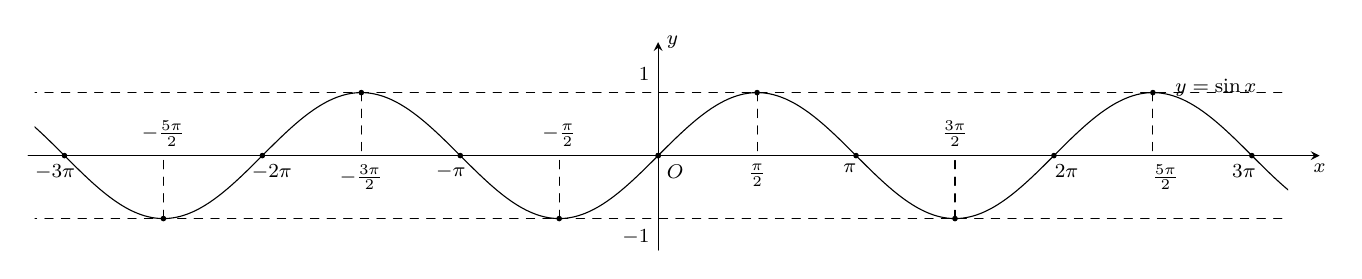
\begin{tikzpicture}[scale=0.8,>=stealth, font=\footnotesize, line join=round, line cap=round]
		\def\xmin{-10} \def\xmax{10.5} \def\ymin{-1.5} \def\ymax{1.8}
		\draw[->] (\xmin,0)--(\xmax,0) node [below]{$x$};
		\draw[->] (0,\ymin)--(0,\ymax) node [right]{$y$};
		\node at (0,0) [below right]{$O$};
		\clip (\xmin+0.1,\ymin+0.1) rectangle (\xmax-0.5,\ymax-0.1);
		\draw[smooth,samples=400,domain=\xmin:\xmax] plot(\x,{sin(\x r)});
		\draw[dashed] (\xmin,1)--(\xmax,1) (\xmin,-1)--(\xmax,-1);
		\foreach \x in {-3*pi,-2.5*pi,-2*pi,-1.5*pi,-pi,-0.5*pi,0}
		{\draw[fill=black] (\x,sin \x*180/pi) circle (1pt);
			\draw[dashed] (\x,sin \x*180/pi)--(\x,0);
			\draw[fill=black] (-\x,sin -\x*180/pi) circle (1pt);
			\draw[dashed] (-\x,sin -\x*180/pi)--(-\x,0);}
		\node at (0,1.3) [left]{$1$};
		\node at (0,-1.3) [left]{$-1$};
		\node at (-2*pi+0.15,0) [below]{$-2\pi$};
		\node at (-3*pi-0.15,0) [below]{$-3\pi$};
		\node at (-2.5*pi,0) [above]{$-\frac{5\pi}{2}$};
		\node at (-1.5*pi,0) [below]{$-\frac{3\pi}{2}$};
		\node at (-pi-0.15,0) [below]{$-\pi$};
		\node at (-0.5*pi,0) [above]{$-\frac{\pi}{2}$};
		\node at (0.5*pi,0) [below]{$\frac{\pi}{2}$};
		\node at (pi-0.1,0) [below]{$\pi$};
		\node at (1.5*pi,0) [above]{$\frac{3\pi}{2}$};
		\node at (2*pi+0.2,0) [below]{$2\pi$};
		\node at (2.5*pi+0.2,0) [below]{$\frac{5\pi}{2}$};
		\node at (3*pi+0.2,0) [below left]{$3\pi$};
		\node at (2.5*pi+1,0.8) [above]{$y=\sin x$};
	\end{tikzpicture}
	\end{center}
	Tìm những giá trị $x$ thuộc  $\left[-\dfrac{3\pi}{2};\dfrac{5\pi}{2}\right]$ để hàm số $y=\sin x$ nhận giá trị âm.
	\loigiai{
		Trên các khoảng $(\pi;0)$; $(\pi;2\pi)$ đồ thị hàm số nằm phía dưới trục hoành nên hàm số $y=\sin x$ nhận giá trị	âm.
	}
\end{bt}

% từ: cau-hoi/lop11/1D1_Ham_so_luong_giac_va_phuong_trinh_luong/1D1-4-8_Toan_thuc_te_ap_dung_ham_so_luong_giac.tex
\begin{bt}%[1D1V4-8]%[ma:806cd6c3]
% nguon: Archive/2024/SP-K10-K11-LyVanHoang_TVN-023/11. C1-LuongGiac-lvhoang_TVN-023/dataC1K11/Bai-3-Dang-6-Dothihamsoluonggiac.tex #2069
[Mức độ 3]%[BG K11, Nhật Thiện]
	Trong Vật lý, phương trình tổng quát của một vật giao động điều hòa cho bởi công thức $x(t)=A\cos (\omega t+\varphi)$, trong đó $t$ là thời điểm (tính bằng giây), $x(t)$ (cm) là li độ của vật tại thời điểm $t$, $A$ là biên độ dao động (độ lệch lớn nhất so với vị trị cân bằng khi vật dao động, $A>0$), $\omega t+\varphi$ là pha của dao động tại thời điểm $t$ và $\varphi\in[-\pi;\pi]$ là pha ban đầu của dao động. Khi đó, chu kỳ $T$ của dao động là $T=\dfrac{2\pi}{\omega}$. Dao động của một con lắc đồng hồ theo thời gian $t$ (giây) được cho bởi đồ thị sau:
	\begin{center}
		\begin{tikzpicture}[line cap=round,line join=round,>=stealth]
			\draw [->] (-2,0)--(10.5,0) node [above right] {$t$};
			\draw [->] (0,-3)--(0,3.5) node [right] {$x$};
			\draw [samples=100, smooth,domain=0:10] plot (\x,{2*cos((\x*pi )r)});
			\foreach \x in {-2,-1,1,2,3,4,5,6,7,8,9,10} \draw (\x,-.045)--(\x,.045) node [below] {$\x$};
			\foreach \x in {-2,-1,1,2,3} \draw (-.045,\x)--(0.045,\x) node [left] {$\x$};
			\path (0,0) node [below left] {$0$};
			\draw[dashed] (0,2) -- (10,2) (0,-2) -- (10,-2);
		\end{tikzpicture}
	\end{center}
	Tính li độ của con lắc tại thời điểm $t=1{,}2$ giây (làm tròn kết quả đến hàng phần mười).  
	\shortans[]{$-1{,}6$}
	\loigiai{Dựa vào đồ thị ta có\\
		Biên độ dao động $A=2$ cm.\\
		Chu kì dao động $T=2$ giây.\\
		Suy ra $\omega=\dfrac{2\pi}{T}=\dfrac{2\pi}{2}=\pi$.\\
		Tại thời điểm ban đầu vật đi từ biên độ dương về vị trí cân bằng nên phương trình li độ có dạng $x=2\cos\left(\pi t\right)$ cm với $\varphi_0=0$.\\
		Tại thời điểm $t=1{,}2$ suy ra $x=2\cos \left(1{,}2\cdot\pi\right)=-1{,}6$.
	}
\end{bt}

% từ: cau-hoi/lop11/1D1_Ham_so_luong_giac_va_phuong_trinh_luong/1D1-4-8_Toan_thuc_te_ap_dung_ham_so_luong_giac.tex
\begin{bt}%[1D1V4-8]%[ma:24c98ff9]
% nguon: Archive/SP_DA_SauLuoi/1-TL-TN-THPT-TruongTHD-GHKI-NH23-24.tex #2571
%[Dự án đề kiểm tra Toán 11 GHKI NH23-24- Thinh Ngo]%[THPT Trần Hưng Đạo]
	Nhiệt độ ngoài trời ở một thành phố vào các thời điểm khác nhau trong ngày có thể được mô phỏng bởi công thức $f(t)=29 + 8\cos\left[\dfrac{\pi}{4}\left( 4-\dfrac{t}{3}\right) \right]$, với $f$ tính bằng độ C và $t$ tính bằng giờ ($0\leq t \leq 24$).
	\begin{enumerate}
		\item Nhiệt độ cao nhất trong ngày là bao nhiêu độ C và vào lúc mấy giờ?
		\item Các công nhân công ty môi trường muốn cắt tỉa các cây trồng ở dải phân cách hai làn đường, họ bắt đầu làm việc từ $6$ giờ và kết thúc lúc $17$ giờ trong ngày. Dựa vào đồ thị hàm số côsin (xem hình bên dưới), hãy cho biết họ nên làm việc vào những thời điểm nào trong ngày để tránh nhiệt độ trên $36^\circ$C (kết quả làm tròn đến hàng phần mười).
		\begin{center}
			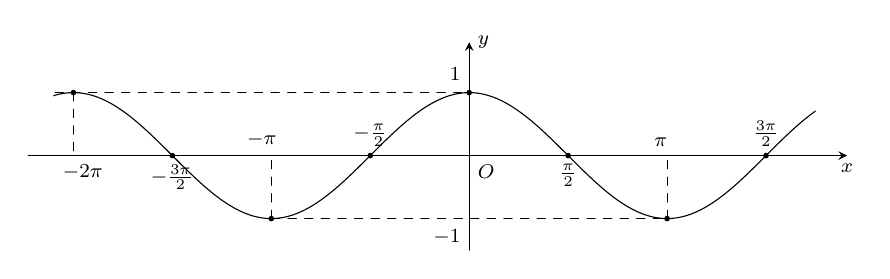
\begin{tikzpicture}[scale=0.8,>=stealth, font=\footnotesize, line join=round, line cap=round]
				\def\xmin{-10} \def\xmax{10.5} \def\ymin{-1.5} \def\ymax{1.8}
				\draw[->] (-7,0)--(6,0) node [below]{$x$};
				\draw[->] (0,\ymin)--(0,\ymax) node [right]{$y$};
				\node at (0,0) [below right]{$O$};
				\clip (\xmin+3.4,\ymin+0.1) rectangle (\xmax-5,\ymax-0.1);
				\draw[smooth,samples=400,domain=\xmin:\xmax] plot(\x,{cos(\x r)});
				\draw[dashed] (\xmin,1)--(0,1) (-3.14,-1)--(3.14,-1);		
				\foreach \x in {-2*pi,-1.5*pi,-pi,-0.5*pi,0}
				{\draw[fill=black] (\x,cos \x*180/pi) circle (1pt);
					\draw[dashed] (\x,cos \x*180/pi)--(\x,0);
					\draw[fill=black] (-\x,cos -\x*180/pi) circle (1pt);
					\draw[dashed] (-\x,cos \x*180/pi)--(-\x,0);}
				\node at (0,1.3) [left]{$1$};
				\node at (0,-1.3) [left]{$-1$};
				\node at (-2*pi+0.15,0) [below]{$-2\pi$};
				\node at (-1.5*pi,0) [below]{$-\frac{3\pi}{2}$};
				\node at (-pi-0.15,0) [above]{$-\pi$};
				\node at (-0.5*pi,0) [above]{$-\frac{\pi}{2}$};
				\node at (0.5*pi,0) [below]{$\frac{\pi}{2}$};
				\node at (pi-0.1,0) [above]{$\pi$};
				\node at (1.5*pi,0) [above]{$\frac{3\pi}{2}$};
			\end{tikzpicture}
		\end{center}
	\end{enumerate} 
	
	\loigiai{
	\begin{enumerate}
		\item Ta có
		\begin{eqnarray*} 
		&-1&\leq \cos\left[\dfrac{\pi}{4}\left( 4-\dfrac{t}{3}\right) \right]\leq 1\\ &\Leftrightarrow& - 8 \leq  8\cos\left[\dfrac{\pi}{4}\left( 4-\dfrac{t}{3}\right) \right]\leq 8\\ &\Leftrightarrow& 21 \leq 29 + 8\cos\left[\dfrac{\pi}{4}\left( 4-\dfrac{t}{3}\right) \right] \leq 37\\
		&\Leftrightarrow& 21 \leq f(t)\leq 37.
		\end{eqnarray*}
	$\text{Max} f(t) = 37$ khi $\cos\left[\dfrac{\pi}{4}\left( 4-\dfrac{t}{3}\right) \right] = 1\Leftrightarrow \dfrac{\pi}{4}\left( 4-\dfrac{t}{3}\right) = k2\pi \Leftrightarrow t = 3(4-8k)$.\\
	Do $0\leq t \leq 24$ cho nên $-\dfrac{1}{2}\leq k \leq \dfrac{1}{2}$ ta chọn $k = 0 \Rightarrow t = 12$.\\ 
	Vậy nhiệt độ cao nhất trong ngày là $37$ độ C vào lúc $12$ giờ.
	\item 
	\begin{center}
		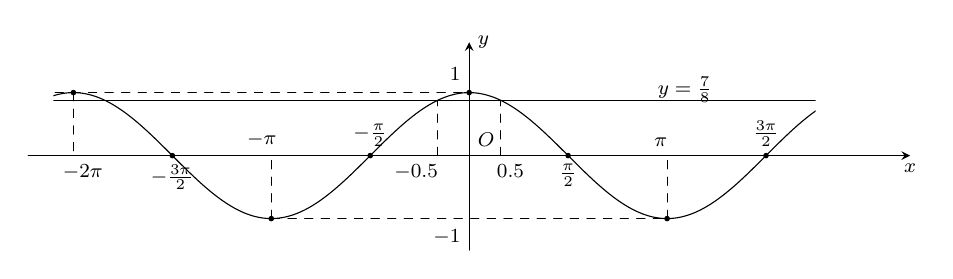
\begin{tikzpicture}[scale=0.8,>=stealth, font=\footnotesize, line join=round, line cap=round]
			\def\xmin{-10} \def\xmax{10.5} \def\ymin{-1.5} \def\ymax{1.8}
			\draw[->] (-7,0)--(7,0) node [below]{$x$};
			\draw[->] (0,\ymin)--(0,\ymax) node [right]{$y$};
			\node at (0,0) [above right]{$O$};
			\clip (\xmin+3.4,\ymin+0.1) rectangle (\xmax-5,\ymax-0.1);
			\draw[smooth,samples=400,domain=\xmin:\xmax] plot(\x,{cos(\x r)});
			\draw[dashed] (\xmin,1)--(0,1) (-3.14,-1)--(3.14,-1);
			\draw
			(\xmin,7/8)--(\xmax,7/8);
			\foreach \x in {-2*pi,-1.5*pi,-pi,-0.5*pi,0}
			{\draw[fill=black] (\x,cos \x*180/pi) circle (1pt);
				\draw[dashed] (\x,cos \x*180/pi)--(\x,0);
				\draw[fill=black] (-\x,cos -\x*180/pi) circle (1pt);
				\draw[dashed] (-\x,cos \x*180/pi)--(-\x,0);}
			\node at (0,1.3) [left]{$1$};
			\node at (0,-1.3) [left]{$-1$};
			\node at (-2*pi+0.15,0) [below]{$-2\pi$};
			\node at (0.161*pi+0.15,0) [below  ]{$0.5$};
			\node at (-0.161*pi+0.15,0) [below left ]{$-0.5$};
			\node at (4.0,0.7) [above left ]{$y = \frac{7}{8}$};
			\node at (-1.5*pi,0) [below]{$-\frac{3\pi}{2}$};
			\node at (-pi-0.15,0) [above]{$-\pi$};
			\node at (-0.5*pi,0) [above]{$-\frac{\pi}{2}$};
			\node at (0.5*pi,0) [below]{$\frac{\pi}{2}$};
			\node at (pi-0.1,0) [above]{$\pi$};
			\node at (1.5*pi,0) [above]{$\frac{3\pi}{2}$};
			\draw[dashed] (0.5,0)--(0.5,7/8);
			\draw[dashed] (-0.5,0)--(-0.5,7/8);
		\end{tikzpicture}
	\end{center}
	Theo đề bài ta có
	\begin{eqnarray*} 
	 &f(t)& \leq 36 \\&\Leftrightarrow& 29 + 8\cos\left[\dfrac{\pi}{4}\left( 4-\dfrac{t}{3}\right) \right] \leq 36\\ &\Leftrightarrow & \cos\left[\dfrac{\pi}{4}\left( 4-\dfrac{t}{3}\right) \right] \leq \dfrac{7}{8}\\& \Leftrightarrow& -0{,}5  \leq \dfrac{\pi}{4}\left( 4-\dfrac{t}{3}\right) \leq 0{,}5\\& \Leftrightarrow& 10{,}1 \leq t \leq 13{,}9.
	 \end{eqnarray*}
	\end{enumerate}

	Như vậy để tránh nhiệt độ trên $36^\circ$C thì các công nhân làm việc từ $10{,1}$ giờ đến $13{,}9$ giờ.
	}
\end{bt}

% từ: cau-hoi/lop11/1D1_Ham_so_luong_giac_va_phuong_trinh_luong/1D1-4-8_Toan_thuc_te_ap_dung_ham_so_luong_giac.tex
\begin{bt}%[1D1C4-8]%[ma:b54bd77b]
% nguon: Archive/SP_DA_SauLuoi/1-TL-THPT-Tenloman-GHKI-NH23-24.tex #2589

\immini{
	\begin{enumerate}
	\item Nếu độ cao của mực nước thủy triều được tính theo công thức $$h(t)=4+2\cos (\dfrac{\pi t}{12}+\dfrac{3\pi}{2})$$ với t là thời gian trong ngày tính theo giờ và độ cao mực nước tính theo đơn vị m. Tính độ cao của mực nước vào lúc 6h sáng.\\
	\item Tuabin gió chuyển đổi động lực di chuyển của gió thành năng lượng điện. Hình bên mô phỏng ba cánh quạt của tuabin gió, các điểm M, N và P là vị trí ban đầu của ba cánh quạt. Giả sử điểm O cách mặt đất 130m và mỗi cánh của tuabin gió dài 70m. Khi điểm N quay được 503 vòng thì khoảng cách từ M đến mặt đất là bao nhiêu biết quạt quay theo chiều kim đồng hồ.(Kết quả làm tròn đến chữ số thập phân thứ hai sau dấu phẩy).
\end{enumerate}}{\begin{tikzpicture}[scale=1, font=\footnotesize, line join=round, line cap=round,>=stealth]  
\def\R{3}
\path
(0,0) coordinate (O)
(20:\R) coordinate (M)
(120:\R) coordinate (N)
(-110:\R) coordinate (P)
(-\R-.2,0) coordinate (E)
(-\R-.2,-2*\R) coordinate (F)
;
\draw[dashed,thick,green] (O) circle (\R);
\draw (N)--(O)--(M) (O)--(P)(E)--(F);

\foreach \x/\g in {O/-45,M/45,N/120,P/-130}\draw[fill=black] (\x) circle (.05) +(\g:.3) node{$\x$};
\draw[fill=black] (E) circle (.05) ;
\draw[fill=black] (F) circle (.05) ;
\node[right] at (-\R-.2,-\R) {$130$ m};
\end{tikzpicture}}
\loigiai{\begin{enumerate}
		\item $\underline{\underline{h}(6)}=6 \mathrm{~m}$
		\item Ta có góc $\widehat{A O M}=15^{\circ}$.Quay 503 vòng thì các điểm vẫn quay lại vị trí ban đầu do đó khoảng cách từ khoảng cách từ $\mathrm{M}$ đến mặt đất là:
		$$
		130+70 \sin \left(15^{\circ}\right)=148.12 m
		$$
	\end{enumerate}
}
\end{bt}

% từ: cau-hoi/lop11/1D1_Ham_so_luong_giac_va_phuong_trinh_luong/1D1-5-3_Phuong_trinh_co_ban_dung_Radian.tex
\begin{ex}%[1D1H5-3]%[ma:d8b4508d]
	\immini[thm]{Phương trình nào dưới đây có tập nghiệm biểu diễn trên  đường tròn lượng giác là $2$ điểm
	$M$, $N$ như trong hình  vẽ?
	 \choice
		{$2\sin 2x=1$} 
		{$2\cos  2x=1$}
		 {\True $2\sin x=1$}
		{$2\cos  x=1$}}
		{\begin{tikzpicture}[scale=1,>=stealth,font=\footnotesize,line join=round,line cap=round]
		\draw[->]  (-1.7,0)--(2.2,0) node[shift={(-120:.2)},scale=1]{$x$};
		\draw[->] (0,-1.7)--(0,1.8)  node[shift={(220:.2)},scale=1]{$y$};
		\path (0,0) coordinate  (O) node[shift={(-135:.25)},scale=1]{$O$};
		\draw (O) circle (1.5cm); 
		 \path
			(30:1.5) coordinate (M) 
			 (150:1.5) coordinate (N);
		 \draw[dashed](M)--(N);
		\draw  (M)--(O)--(N);
		\fill (M) node[shift={(30:.25)}]{$M$}circle (1pt); 
		\fill (N) node[shift={(150:.2)}]{$N$}circle (1pt); 
		\fill (0,0.75)  node[shift={(145:.3)}]{$0{,}5$}circle (1pt);
		 \fill (1.5,0) node[shift={(-50:.2)}]{$1$}circle (1pt);
	\end{tikzpicture}
		 }
	\loigiai{ 
		Ta thấy $2$ điểm $M$ và $N$ là các giao điểm của đường thẳng vuông góc với trục tung tại điểm $\dfrac{1}{2}$ với đường tròn lượng giác nên $M$ và $N$ là các điểm biểu diễn tập nghiệm của phương trình lượng giác cơ bản $\sin x=\dfrac{1}{2}\Leftrightarrow 2\sin  x=1$.
	} 
\end{ex}

% từ: cau-hoi/lop11/1D1_Ham_so_luong_giac_va_phuong_trinh_luong/1D1-5-4_Phuong_trinh_co_ban_dung_Do.tex
\begin{bt}%[1D1H5-4]%[ma:1e54948c]
% nguon: Archive/2024/TOAN_11_XE/TOAN_11_XE/data4/11C1/KNTT-1.4.tex #1094
%[Tex hóa SGK 11, KNTT]
	Giải các phương trình sau:
	\begin{multicols}{2}
	\begin{enumerate}
		\item $\sin x=\dfrac{\sqrt{3}}{2}$.
		\item  $2\cos x=-\sqrt2$.
		\item $\sqrt3\tan\left(\dfrac{x}{2}+15^\circ \right)=1$.
		\item $\cot(2x-1)=\cot\dfrac{\pi}{5}$. 
	\end{enumerate}
	\end{multicols}
	\loigiai{
		\begin{enumerate}
			\item $\sin x=\dfrac{\sqrt{3}}{2}\Leftrightarrow \sin x=\sin\left( \dfrac{\pi}{3} \right) \Leftrightarrow \hoac{&x=\dfrac{\pi}{3}+k2\pi\\&x=\dfrac{2\pi}{3}+k2\pi}, k \in \mathbb{Z}$.
			\item $2\cos x=-\sqrt2 \Leftrightarrow \cos x=-\dfrac{\sqrt2}{2} \Leftrightarrow \cos x=\cos\left(\dfrac{3\pi}{4} \right)  \Leftrightarrow \hoac{&x=\dfrac{3\pi}{4}+k2\pi\\&x=-\dfrac{3\pi}{4}+k2\pi}, k \in \mathbb{Z}$.
			\item $\sqrt3\tan\left(\dfrac{x}{2}+15^\circ \right)=1 \Leftrightarrow \tan \left(\dfrac{x}{2}+15^\circ \right)=\dfrac{1}{\sqrt3} \Leftrightarrow \tan \left(\dfrac{x}{2}+15^\circ \right)=\tan\left(30^\circ \right) \\ \Leftrightarrow \dfrac{x}{2}+15^\circ=30^\circ+k180^{\circ} \Leftrightarrow x=30^\circ+k360^{\circ}, k \in \mathbb{Z}$.
			\item $\cot(2x-1)=\cot\dfrac{\pi}{5} \Leftrightarrow 2x-1=\dfrac{\pi}{5} +k\pi, x=\dfrac{1}{2}+\dfrac{\pi}{10}+\dfrac{k}{2}\pi, k \in \mathbb{Z}$.
		\end{enumerate}
	}
\end{bt}

% từ: cau-hoi/lop11/1D2_Day_so_Cap_so_cong_Cap_so_nhan/1D2-1-1_Cau_hoi_ly_thuyet.tex
\begin{bt}%[1D2Y1-1]%[ma:bf634069]
	Trong các dãy số $(u_n)$ sau, dãy số nào bị chặn  dưới, bị chặn trên, bị chặn?
	\begin{enumEX}[a)]{4}
		\item  $u_n=n-1$;
		 \item $u_n=\dfrac{n+1}{n+2}$;
		\item $u_n=\sin  n$;
		 \item $u_n=(-1)^{n-1} n^2$.
	\end{enumEX}
	\loigiai{\begin{enumEX}[a)]{1}
		\item  Dãy số $u_n=n-1$ bị chặn dưới, vì $u_{n}\ge 0,\, \forall n \in \mathbb{N}^{*}$.
		\item Dãy số $u_n=\dfrac{n+1}{n+2}$  bị chặn trên, vì $u_n=1-\dfrac{1}{n+2}<1,\, \forall n \in \mathbb{N}^{*}$.\\
		Dãy số $\left(u_{n}\right)$ cũng bị chặn dưới, vì $u_n=\dfrac{n+1}{n+2} \geq \dfrac{2}{3},\, \forall  n \in \mathbb{N}^{*}$.\\
		 Vậy dãy số $\left(u_{n}\right)$ bị chặn.
		\item Dãy số $u_n=\sin n$ bị chặn trên, bị chặn dưới, vì $-1\le \sin n  \le1,\, \forall n \in \mathbb{N}^{*}$.\\
		 Vậy dãy số $\left(u_{n}\right)$ bị chặn.
		\item Bốn  số hạng đầu của dãy số là \\$u_2=(-1)^1\cdot 2^2=-4;$ $u_3=(-1)^2\cdot 3^2=9;$ $u_4=(-1)^3 \cdot 4^2=-16;$ $u_5=(-1)^4\cdot 5^2=25;$ $\cdots$
		 \\
		Vậy dãy số không  bị chặn.
\end{enumEX}}
\end{bt}

% từ: cau-hoi/lop11/1D2_Day_so_Cap_so_cong_Cap_so_nhan/1D2-1-4_Day_so_tang_day_so_giam.tex
\begin{bt}%[1D2H1-4]%[ma:5c5917ec]
% nguon: Archive/SP_KhoLatex/ID6_old/1K2-5.tex #3380
%[Dự án 2 - TLDH - TeamTeXHoa - Nguyễn Cường]
	Xét tính đơn điệu của các dãy số sau
	\begin{multicols}{2}
		\begin{enumerate}
			\item $u_n=\dfrac{2n^2-1}{n^2+1}$;
			\item $u_n=\sqrt{n+1}-\sqrt{n}$.
		\end{enumerate}
	\end{multicols}
	\loigiai 
	{
		\begin{enumerate}
			\item Ta có $u_n=\dfrac{2n^2-1}{n^2+1}=2-\dfrac{3}{n^2+1}$ và $u_{n+1}=2-\dfrac{3}{(n+1)^2+1}$.\\
			Với mọi $n\in \mathbb{N}^*$, ta có
			\allowdisplaybreaks
			\begin{eqnarray*}
				(n+1)^2>n^2&\Leftrightarrow&\dfrac{1}{(n+1)^2+1}<\dfrac{1}{n^2+1}\\
				&\Leftrightarrow&2-\dfrac{3}{(n+1)^2+1}>2-\dfrac{3}{n^2+1}\\
				&\Leftrightarrow& u_{n+1}>u_n.
			\end{eqnarray*}
			Suy ra dãy số đã cho là dãy số tăng.
			\item Ta có $u_n=\sqrt{n+1}-\sqrt{n}=\dfrac{1}{\sqrt{n+1}+\sqrt{n}}$ và $u_{n+1}=\dfrac{1}{\sqrt{n+2}+\sqrt{n+1}}$.\\
			Với mọi $n\in \mathbb{N}^*$, ta có
			\allowdisplaybreaks
			\begin{eqnarray*}
				(\sqrt{n+2}+\sqrt{n+1}>\sqrt{n+1}+\sqrt{n}&\Leftrightarrow&\dfrac{1}{\sqrt{n+2}+\sqrt{n+1}}<\dfrac{1}{\sqrt{n+1}+\sqrt{n}}\\
				&\Leftrightarrow& u_{n+1}<u_n.
			\end{eqnarray*}
			Suy ra dãy số đã cho là dãy số giảm.
		\end{enumerate}
	}
\end{bt}

% từ: cau-hoi/lop11/1D2_Day_so_Cap_so_cong_Cap_so_nhan/1D2-1-4_Day_so_tang_day_so_giam.tex
\begin{bt}%[1D2H1-4]%[ma:a566ce13]
% nguon: Archive/SP_KhoLatex/ID6_old/1K2-5.tex #3402
%[Dự án 2 - TLDH - TeamTeXHoa - Đào Trung Kiên]%[ID6]
	Xét tính tăng, giảm của dãy số $\left(u_n\right)$, biết
	\begin{multicols}{3}
		\begin{enumerate}
			\item $u_n=2 n-1$;
			\item  $u_n=-3 n+2$;
			\item  $u_n=\dfrac{(-1)^{n-1}}{2^n}$.
		\end{enumerate}
	\end{multicols}
	\loigiai{
		\begin{enumerate}
			\item  Ta có $u_{n+1}-u_n=2>0,\forall n \in \mathbb{N}^*$ suy ra đây là dãy số tăng.
			\item  Ta có $u_{n+1}-u_n=-3<0,\forall n \in \mathbb{N}^*$ suy ra đây là dãy số giảm.
			\item  $u_3=\dfrac{1}{8}>u_2=\dfrac{-1}{4}<u_1=\dfrac{1}{2}$ suy ra đây là dãy số không tăng không giảm.
		\end{enumerate}
	}	
\end{bt}

% từ: cau-hoi/lop11/1D2_Day_so_Cap_so_cong_Cap_so_nhan/1D2-3-4_Tim_so_hang_cu_the_trong_cap_so_nhan.tex
\begin{ex}%[1D2H3-4]%[ma:d54adfbd]
	Giả sử $\dfrac{\sin \alpha}{6},\, \cos \alpha,\, \tan \alpha$ theo thứ tự đó là một cấp  số nhân. Tính $\cos 2 \alpha$.
	 \choice
		{$-\dfrac{\sqrt{3}}{2}$} 
		 {$\dfrac{1}{2}$}
		{\True $-\dfrac{1}{2}$} 
		{$\dfrac{\sqrt{3}}{2}$} 
	 \loigiai{
		Điều kiện $\cos \alpha \neq 0 \Leftrightarrow \alpha \neq \dfrac{\pi}{2}+k \pi(k \in \mathbb{Z}$).\\ 
		 Theo tính chất của cấp số nhân, ta có
		$$\begin{aligned}
		&\cos ^2 \alpha=\dfrac{\sin  \alpha}{6} \cdot \tan \alpha\\
		&\Leftrightarrow 6 \cos ^2 \alpha=\dfrac{\sin ^2 \alpha}{\cos \alpha}\\ 
		&\Leftrightarrow 6 \cos ^3  \alpha-\sin ^2 \alpha=0\\
		&\Leftrightarrow 6 \cos ^3 \alpha+\cos  ^2 \alpha-1=0\\
		&\Leftrightarrow\cos  \alpha=\dfrac{1}{2}.
	\end{aligned}$$
	Ta có $\cos 2 \alpha=2 \cos ^2 \alpha-1=2  \cdot\left(\dfrac{1}{2}\right)^2-1=-\dfrac{1}{2}$.
} 
\end{ex}

% từ: cau-hoi/lop11/1D2_Day_so_Cap_so_cong_Cap_so_nhan/1D2-3-4_Tim_so_hang_cu_the_trong_cap_so_nhan.tex
\begin{ex}%[1D2V3-4]%[ma:f5131e8c]
	Giả sử $\dfrac{\sin \alpha}{6}$, $\cos \alpha$, $\tan \alpha$ theo thứ tự đó là một cấp số  nhân. Tính $\cos 2\alpha$.
	\choice 
		{  $\dfrac{\sqrt{3}}{2}$ }
		{ $-\dfrac{\sqrt{3}}{2}$ } 
		 { $\dfrac{1}{2}$ }
		{ \True $-\dfrac{1}{2}$ } 
	\loigiai{ 
		Điều kiện $\cos \alpha \ne 0 \Leftrightarrow \alpha \ne \dfrac{\pi}{2} + k\pi\quad  (k \in \mathbb{Z})$.\\
		Theo tính chất của cấp  số nhân, ta có
		\begin{eqnarray*}
			&&\cos^2 \alpha = \dfrac{\sin  \alpha}{6} \cdot \tan \alpha = \dfrac{\sin^2 \alpha}{6\cos \alpha}\\
			&\Rightarrow& 6 \cos^3 \alpha  - \sin^2 \alpha = 0\\ &\Leftrightarrow& 6 \cos^3 \alpha + \cos^2 \alpha - 1 = 0\\
			 &\Leftrightarrow& \cos \alpha = \dfrac{1}{2}.
		\end{eqnarray*}
		Ta có: $\cos 2\alpha = 2 \cos^2 \alpha - 1 = 2 \cdot \left( \dfrac{1}{2} \right)^2 - 1 = \dfrac{1}{2} - 1  = -\dfrac{1}{2}$.
	 }
\end{ex}

% từ: cau-hoi/lop11/1D2_Day_so_Cap_so_cong_Cap_so_nhan/1D2-3-5_Dieu_kien_de_day_so_la_cap_so_nhan.tex
\begin{ex}%[1D2V3-5]%[ma:acc80850]
	Giả sử $\dfrac{\sin\alpha}{6}$, $\cos\alpha $, $\tan\alpha $ theo thứ tự đó là một  cấp số nhân. Tính $\cos 2\alpha $.
	 \choice
		{$\dfrac{\sqrt  3}{2}$}
		{$-\dfrac{\sqrt 3}{2}$} 
		 {$\dfrac{1}{2}$}
		{\True $-\dfrac{1}{2}$} 
	 \loigiai{
		Điều kiện $\cos\alpha\ne  0 \Leftrightarrow\alpha\ne\dfrac{\pi}{2}+k\pi $.\\
		Theo tính chất của  cấp số nhân, ta có\\
		$\cos  ^2\alpha=\dfrac{\sin\alpha}{6} \cdot \tan\alpha \Leftrightarrow 6\cos ^2\alpha=\dfrac{\sin^2\alpha}{\cos\alpha}\\
		\Leftrightarrow 6\cos  ^3\alpha-\sin ^2\alpha=0 \Leftrightarrow 6\cos ^3\alpha+\cos ^2\alpha-1=0 \Leftrightarrow\cos\alpha=\dfrac{1}{2}$.\\
	Ta có $\cos  2\alpha=2\cos ^2\alpha-1=2 \cdot \left(\dfrac{1}{2}\right)^2-1=-\dfrac{1}{2}$.}
\end{ex}

% từ: cau-hoi/lop11/1D2_Day_so_Cap_so_cong_Cap_so_nhan/1D2-3-6_Tinh_tong_cua_cap_so_nhan.tex
\begin{ex}%[1D2H3-6]%[ma:904c4b8e]
	Cho dãy số $\left(u_n\right)$ xác định bởi  $u_1=2$ và $u_{n+1}=\dfrac{n+1}{2n} \cdot u_n$. Xét tính đúng sai của các mệnh đề sau
	\choiceTF 
		 {\True Số hạng $u_2=2$}
		{Tỉ  số $\dfrac{u_{2\,023}}{u_{2024}}=2$}
		{Số hạng  $u_{2024}=\dfrac{1}{2^{2024}}$}
		{\True Tổng  $S=u_1+\dfrac{u_2}{2}+\dfrac{u_3}{3}+\ldots+\dfrac{u_{10}}{10}$ bằng $\dfrac{1\,023}{256}$}
	 \loigiai{
		Theo đề ta có $u_{n+1}=\dfrac{n+1}{2 n} \cdot u_n \Leftrightarrow  \dfrac{u_{n+1}}{n+1}=\dfrac{u_n}{2n}$.\\
		Đặt  $v_n=\dfrac{u_n}{n}$ thì $v_{n+1}=\dfrac{1}{2} v_n$.\\
		Do đó $\left(v_n\right)$ là một cấp số nhân với  $v_1=\dfrac{u_1}{1}=2$ và công bội $q=\dfrac{1}{2}$.\\
		Số  hạng tổng quát của dãy $\left(v_n\right)$ là $v_n=v_1 \cdot q^{n-1}=2 \cdot\left(\dfrac{1}{2}\right)^{n-1}=\left(\dfrac{1}{2}\right)^{n-2} \Rightarrow u_n=n \cdot\left(\dfrac{1}{2}\right)^{n-2}$.
		\begin{itemchoice}
			\itemch \textbf{Đúng} \\ 
			Số hạng $u_2=2\cdot  \left(\dfrac{1}{2}\right)^{2-2}=2$.
			\itemch \textbf{Sai} \\ 
			 Ta có $\dfrac{u_n}{u_{n+1}}=\dfrac{2n}{n+1} \Rightarrow \dfrac{u_{2\,023}}{u_{2024}}=\dfrac{2\cdot 2\,023}{2\,024}=\dfrac{2\,023}{1\,012}$.
			\itemch \textbf{Sai} \\ 
			Ta có $u_{2\,024}=2\,024  \cdot\left(\dfrac{1}{2}\right)^{2022}=253 \cdot\left(\dfrac{1}{2}\right)^{2019}$.
			\itemch \textbf{Đúng} \\ 
			Ta có $v_n=\dfrac{u_n}{n}=\left(\dfrac{1}{2}\right)^{n-2}$ là một cấp  số nhân với $v_1=\dfrac{u_1}{1}=2$ và công bội $q=\dfrac{1}{2}$.\\
			Khi  đó $S=u_1+\dfrac{u_2}{2}+\dfrac{u_3}{3}+\ldots+\dfrac{u_{10}}{10}=v_1\dfrac{1-q^{10}}{1-q}=2\cdot \dfrac{1-\left(\dfrac{1}{2}\right)^{10} }{1-\dfrac{1}{2}}=\dfrac{1\,023}{256}$.
		\end{itemchoice}
	 }
\end{ex}

% từ: cau-hoi/lop11/1D3_Gioi_han_Ham_so_lien_tuc/1D3-1-2_Phuong_phap_dat_thua_so_chung_lim_huu_han.tex
\begin{ex}%[1D3H1-2]%[ma:f8161cce]
	Tính các  giới hạn sau đây
	\begin{listEX}[3]
		\item $\lim \dfrac{-2n+1}{n}$. 
		 \item $\lim \dfrac{\sqrt{16n^2-2}}{n}$.
		\item $\lim  \dfrac{4}{2n+1}$.
		 \item $\lim \dfrac{n^2-2n+3}{2n^2}$.
		 \item $\lim \dfrac{1}{-3n+7}$.
		 \item $\lim \dfrac{2}{(n+1)(n-2)}$.
		\item  $\lim \dfrac{3}{2^n+1}$.
		\item $\lim \dfrac{2^n}{5+7^n}$. 
		 \item $\lim \dfrac{-3n^2+4n+1}{2n^3-3n+7}$.
		 \item $\lim \dfrac{(2n+1)(n-2)+n}{n^3+n}$.
		\item $\lim  \dfrac{4\cdot 3^n+5^n}{2\cdot 5^n+7^n}$.
		 \item $\lim \dfrac{4^n+7^n}{\left(2^n+1\right)\left(5+7^n\right)}$.
	\end{listEX}
	\loigiai{ 
		\begin{enumerate}
			\item $\lim  \dfrac{-2n+1}{n}=\lim \left(-2+\dfrac{1}{n}\right)=-2$.
			\item $\lim \dfrac{\sqrt{16n^2-2}}{n}=\lim \sqrt{\dfrac{16n^2-2}{n^2}}=\sqrt{\lim  \left(16-\dfrac{2}{n^2}\right)}=\sqrt{16}=4$.
			\item  $\lim \dfrac{4}{2n+1}=\lim \dfrac{\dfrac{4}{n}}{2+\dfrac{1}{n}}=\dfrac0{2+0}=0$.
			\item $\lim  \dfrac{n^2-2n+3}{2n^2}=\lim \left(\dfrac{1}{2}-\dfrac{1}{n}+\dfrac{3}{2n^2}\right)=\dfrac{1}{2}$.
			\item $\lim \dfrac{1}{-3n+7}=\lim \dfrac{1}{n} \cdot  \dfrac{1}{\left(-3+\dfrac{7}{n}\right)}=0\cdot \dfrac{1}{-3+0}=0$.
			 \item $\lim \dfrac{2}{(n+1)(n-2)}=\lim \dfrac{1}{n^2} \cdot \dfrac{1}{\left(1+\dfrac{1}{n}\right)\left(1-\dfrac{2}{n}\right)}=0\cdot \dfrac{1}{(1+0)(1-0)}=0$.
			\item $\lim \dfrac{3}{2^n+1}=\lim \left(\dfrac{1}{2}\right)^n \cdot \dfrac{3}{1+\left(\dfrac{1}{2}\right)^n}=0\cdot \dfrac{3}{1+0}=0$. 
			\item $\lim \dfrac{2^n}{5+7^n}=\lim \left(\dfrac{2}{7}\right)^n  \cdot \dfrac{1}{5\cdot\left(\dfrac{1}{7}\right)^n+1}=0\cdot \dfrac{1}{5\cdot 0+1}=0$.
			 \item $\lim \dfrac{-3n^2+4n+1}{2n^3-3n+7}=\lim \dfrac{1}{n} \cdot\left(\dfrac{-3+\dfrac{4}{n}+\dfrac{1}{n^2}}{2-\dfrac{3}{n^2}+\dfrac{7}{n^3}}\right)=0\cdot \dfrac{-3+0+0}{2-0+0}=0$.
			\item $\lim \dfrac{(2n+1)(n-2)+n}{n^3+n}=\lim \dfrac{2n^2-2n-2}{n^3+n}=\lim \dfrac{1}{n}  \cdot\left(\dfrac{2-\dfrac{2}{n}-\dfrac{2}{n^2}}{1+\dfrac{1}{n^2}}\right)=0\cdot \dfrac{2-0-0}{1+0}=0$.
			\item $\lim \dfrac{4\cdot  3^n+5^n}{2\cdot 5^n+7^n}=\lim \left(\dfrac{5}{7}\right)^n\left(\dfrac{4\cdot\left(\dfrac{3}{5}\right)^n+1}{2\cdot\left(\dfrac{5}{7}\right)^n+1}\right)=0\cdot \dfrac{4\cdot 0+1}{2\cdot 0+1}=0$.
			\item $\lim  \dfrac{4^n+7^n}{\left(2^n+1\right)\left(5+7^n\right)}=\lim \left(\dfrac{1}{2}\right)^n\left(\dfrac{\left(\dfrac{4}{7}\right)^n+1}{\left(1+\left(\dfrac{1}{2}\right)^n\right)\left(5.\left(\dfrac{1}{7}\right)^n+1\right)}\right)=0$.
		\end{enumerate}
	 }
\end{ex}

% từ: cau-hoi/lop11/1D3_Gioi_han_Ham_so_lien_tuc/1D3-1-2_Phuong_phap_dat_thua_so_chung_lim_huu_han.tex
\begin{ex}%[1D3H1-2]%[ma:ddbad7b7]
	Tìm  giới hạn của các dãy số sau
	\begin{listEX}[3]
		\item  $u_n=\dfrac{-3n^3+2n^2+1}{2n^3-n}$.
		 \item $u_n=\dfrac{2n+1}{n^2+n+3}$.
		\item  $u_n=\dfrac{2025n+2024}{n-2023}$.
	\end{listEX}
	\loigiai{ 
		\begin{enumerate}
			 \item Ta có $\lim u_n=\lim \dfrac{-3n^3+2n^2+1}{2n^3-n}=\lim \dfrac{n^3\left(-3+\dfrac{2}{n}+\dfrac{1}{n^3}\right)}{n^3\left(2-\dfrac{1}{n^2}\right)}=\lim \dfrac{-3+\dfrac{2}{n}+\dfrac{1}{n^3}}{2-\dfrac{1}{n^2}}=-\dfrac{3}{2}$.
			\item  Ta có $\lim u_n=\lim \dfrac{2n+1}{n^2+n+3}=\lim \dfrac{n\left(2+\dfrac{1}{n}\right)}{n^2\left(1+\dfrac{1}{n}+\dfrac{3}{n^2}\right)}=\lim \left(\dfrac{1}{n} \cdot \dfrac{\dfrac{2}{n}+\dfrac{1}{n^2}}{1+\dfrac{1}{n}+\dfrac{3}{n^2}}\right)=0$.
			\item Ta có $\lim u_n=\lim  \dfrac{2025n+2024}{n-2023}=\lim \dfrac{n\left(2025+\dfrac{2024}{n}\right)}{n\left(1-\dfrac{2023}{n}\right)}=\lim \dfrac{2025+\dfrac{2024}{n}}{1-\dfrac{2023}{n}}=2025$.
		\end{enumerate}
	 }
\end{ex}

% từ: cau-hoi/lop11/1D3_Gioi_han_Ham_so_lien_tuc/1D3-3-2_Tinh_lien_tuc_the_hien_qua_do_thi.tex
\begin{ex}%[1D3N3-2]%[ma:b9f54b9a]
	\immini{ 
	Cho đồ  thị hàm số $y=f(x)$ có đồ thị như hình vẽ bên. Chọn mệnh đề đúng trong các mệnh đề sau
	\choice 
		{Hàm số $y=f(x)$ gián đoạn  tại $x_0 = 0$}
		{$\displaystyle\lim\limits_{x \rightarrow +\infty} f\left(x\right)  = -1$}
		{$\displaystyle\lim\limits_{x  \rightarrow -\infty} f\left(x\right) = -1$}
		{\True Hàm số $y=f(x)$ liên tục trên $\mathbb{R}$}}{ 
		\begin{tikzpicture}[>=stealth,scale=0.8]
				\draw[->] (-2,0)--(0,0)  node[below left]{$O$}--(4,0) node[above]{$x$};
				\draw[->,color=black]  (0,-2)--(0,4) node[right]{$y$};
				\clip (-3,-3) rectangle  (4,4);
				\draw (-2,-2)--(-0.5,1.2)--(0,0)--(1.5,3.2)--(3.9,-2)  node[left]{$y=f (x)$};
				 \draw[dashed] (-2,-1)--(4,-1);
				\draw[fill] (0,-1) circle (1.3pt) node[below  left]{$-1$};
				\draw[fill]  (-1.05,0) circle (1.3pt) node[above left]{$-1$};
			\end{tikzpicture}
		 }
	\loigiai{ 
		Quan sát đồ  thị hàm số, ta có
		\begin{enumerate}[$\bullet$]
			\item Đồ thị hàm số là các đường liền nét trên khoảng $\left(-\infty;+\infty\right)$  do đó hàm số liên tục trên $\mathbb{R}$.
			\item $\displaystyle\lim\limits_{x  \rightarrow +\infty} f\left(x\right) = -\infty$.
			 \item $\displaystyle\lim\limits_{x \rightarrow -\infty} f\left(x\right) = -\infty$.
		\end{enumerate}
	} 
\end{ex}

% từ: cau-hoi/lop11/1D3_Gioi_han_Ham_so_lien_tuc/1D3-3-2_Tinh_lien_tuc_the_hien_qua_do_thi.tex
\begin{ex}%[1D3V3-2]%[ma:9c580735]
	 [Dự án 11HVA 2024-2025]
	Cho hàm số $y=f(x)$ có đồ thị  như hình vẽ dưới đây:
	\begin{center}
		\begin{tikzpicture}[>=stealth,scale=1.2]
				\def\xmin{-1} \def\xmax{6} 
				\def\ymin{-2}  \def\ymax{6}
				 \draw[->] (-1,0) -- (6,0) node[right] {$x$};
				\draw[->]  (0,-2) -- (0,6) node[above] {$y$};
				\clip  (\xmin+0.1,\ymin+0.1) rectangle (\xmax+0.2,\ymax-0.1);
				\draw[dashed]  (1,-2) -- (1,6);
				\draw[dashed]  (4,-2) -- (4,6);
				 \draw[dashed] (-1,2) -- (6,2);
				\draw  (-1,3) -- (6,3);
				 \node at (0.2,-0.3) {O};
				\node  at (1,-0.3) {1};
				\node at (4,-0.3)  {4};
				\node  at (-0.3,2) {2};
				\node  at (-0.3,3) {3};
				\draw[domain=0:0.95,samples=100] 
					plot (\x,{1/(\x-1)  + 4});
				 \draw[domain=-1:0,samples=100]
					plot (\x,{-2/(\x-2)  +2});
				 \draw[domain=1.2:3.8,samples=100]
					plot (\x,{1*(\x-2.5)^2+  4});
				\draw[domain=4.05:5.95,smooth] plot  ({\x},{-1/(\x-4)+3.5});
			\end{tikzpicture}
	\end{center}
	 \choiceTF
		{\True Hàm  số liên tục tại điểm $x=0$}
		{Hàm số liên tục  tại điểm $x=1$}
		{Hàm  số liên tục trên $(0;+\infty)$}
		{\True Hàm số liên tục trên  $(1; 4)$}
	\loigiai{Tại lân cận điểm $x=0$ thì hàm số là đường liền nét khi đi  qua điểm $x=0$ nên hàm số liên tục tại điểm $x=0$.\\
		Tại lân cận điểm $x=1$ thì hàm số  là đường đứt đoạn khi đi qua điểm $x=1$ nên hàm số gián đoạn tại điểm $x=1$.\\
		Vì hàm số gián đoạn tại điểm $x=1$ nên hàm số không liên tục trên $(0;+\infty)$.\\ 
		Vì hàm số liên tục tại mọi điểm $x \in(1; 4)$ nên hàm số liên tục  trên $(1; 4)$.
		\begin{itemchoice}
			\itemch \textbf{Đúng.}  \\
			Hàm số  liên tục tại điểm $x=0$.
			\itemch \textbf{Sai.} \\ 
			Hàm số  gián đoạn tại điểm $x=1$.
			\itemch \textbf{Sai.}  \\
			Hàm  số không liên tục trên $(0;+\infty)$.
			 \itemch \textbf{Đúng.} \\
			 Hàm số liên tục trên $(1; 4)$.
		\end{itemchoice}
	 }
\end{ex}

% từ: cau-hoi/lop11/1D3_Gioi_han_Ham_so_lien_tuc/1D3-3-5_Bai_toan_phuong_trinh_co_nghiem.tex
\begin{ex}%[1D3H3-5]%[ma:1e5d8309]
	Tìm tất cả các giá trị của tham số thực sao cho phương trình sau có  nghiệm:\break $(2m^2-5m+2)(x-1)^{2017}(x^{2018}-2)+2x+3=0$.
	 \loigiai{
		\begin{itemize}
			\item Nếu $2m^2-5m+2=0$ thì phương trình đã cho trở thành $2x+3=0  \Leftrightarrow x=-\dfrac{3}{2}$.
			\item Nếu $2m^2-5m+2\ne 0$ phương trình đã cho là một đa thưc bậc  lẻ nên phương trình có ít nhất một nghiệm.
		\end{itemize}
		 Vậy với mọi phương trình đã cho luôn có ít nhất một nghiệm.
	} 
\end{ex}

% từ: cau-hoi/lop11/1D3_Gioi_han_Ham_so_lien_tuc/1D3-3-5_Bai_toan_phuong_trinh_co_nghiem.tex
\begin{ex}%[1D3V3-5]%[ma:e2ed179b]
	Chứng minh rằng với mọi  giá trị của tham số $m$ phương trình $(1-m^2)x^5-3x-1=0$ luôn có nghiệm.
	 \loigiai{
		Xét hàm số $f(x)=(1-m^2)x^5-3x-1$ là hàm số liên tục trên $\mathbb{R}$ nên nó liên tục trên  $[-1; 0]$.\\
		Ta có $f(0)=-1$ và $f(-1)=m^2+1$ nên $f(0) \cdot f(-1) < 0, \forall m \in  \mathbb{R}$.\\
		Khi đó phương trình  $f(x)=0$ có ít nhất một nghiệm trong khoảng $(-1; 0)$.\\
		Vậy phương trình $(1-m^2)x^5-3x-1=0$ luôn có ít nhất một  nghiệm.
	} 
\end{ex}

% từ: cau-hoi/lop11/1D6_Ham_so_mu_va_ham_so_logarit/1D6-3-3_Su_bien_thien_va_do_thi_cua_ham_so_mu_logarit.tex
\begin{ex}%[1D6N3-3]%[ma:8c261dbb]
	\immini{Đồ thị hàm số nào dưới đây có  dạng như đường cong trong hình bên?
	\choice 
		{$  y=\mathrm{e}^x$}
		 {\True $ y=\log_{\sqrt{7}}x$}
		{$  y=\log_{\frac{1}{2}}x$}
		{$  y=\dfrac{1}{\mathrm{e}^x}$}
		} 
		 {
		\begin{tikzpicture}[>=stealth,scale=1,font=\footnotesize,line join=round,line cap=round]
				\def\a{1} \def\b{0}  \def\c{-3} \def\d{1}
				\def\xt{-1} \def\xp{3} \def\yt{2}  \def\yd{-1.5}
				\draw (1,0) circle (1pt)  node[below]{$1$}
					 (0,-1) circle (1pt) node[left]{$-1$}
					(0,1)  circle (1pt) node[left]{$1$}
					 (2,0) circle (1pt) node[below]{$2$};
				\draw[->] (\xt,0)--(\xp,0) node  [below]{$x$};
				\draw[->]  (0,\yd)--(0,\yt) node [left]{$y$};
				\node at (0,0)  [below right]{$O$};
				 \clip (\xt-0.1,\yd+0.1) rectangle (\xp-0.1,\yt-0.1);
				\draw[smooth,domain=0.1:3]  plot (\x,{ln(\x)/(ln(2.6457))});
			\end{tikzpicture}
		 }
	\loigiai{ 
		 Đồ thị hàm số nhận trục $Oy$ làm tiệm cận đứng nên đây là hàm số logarit $ y={{\log }_a}x$, ta loại phương án $y=\mathrm{e}^x$ và $y=\dfrac{1}{\mathrm{e}^x}$.\\
		Dựa vào đồ  thị, hàm số đồng biến trên $(0;+\infty)$ nên $a>1$, loại phương án $y=\log_{\frac{1}{2}}x$.\\
	Vậy ta chọn phương án  $y=\log_{\sqrt{7}}x$.}
\end{ex}

% từ: cau-hoi/lop11/1D6_Ham_so_mu_va_ham_so_logarit/1D6-3-3_Su_bien_thien_va_do_thi_cua_ham_so_mu_logarit.tex
\begin{ex}%[1D6N3-3]%[ma:14cb49f0]
	Tìm hàm số đồng biến  trên $\mathbb{R}$.
	\choice 
		{\True  $f(x)=3^x$}
		{$f(x)=3^{-x}$} 
		{$f(x)=\left(\dfrac{1}{\sqrt{3}}\right)^x$} 
		{$f(x)=\dfrac{3}{3^x}$} 
	 \loigiai{
		Vì $3>1$ nên hàm số $f(x)=3^x$ đồng biến trên $\mathbb{R}$. 
	 }
\end{ex}

% từ: cau-hoi/lop11/1D6_Ham_so_mu_va_ham_so_logarit/1D6-3-3_Su_bien_thien_va_do_thi_cua_ham_so_mu_logarit.tex
\begin{ex}%[1D6N3-3]%[5-CTST]%[ma:f7edebf3]
	Tìm hàm  số đồng biến trên $\mathbb{R}$.
	 \choice
		 {\True $f(x) = 3^x$}
		{$f(x) = 3^{-x}$} 
		 {$f(x) = \left(\dfrac{1}{\sqrt{3}} \right)^{x}$}
		{$f(x) = \dfrac{3}{3^x}$} 
	\loigiai{ 
		Hàm số $f(x) = a^x$ đồng biến trên $\mathbb{R}$ nếu $a > 1$.\\ 
		Do đó hàm số $fx) = 3^x$ là hàm số đồng biến trên $\mathbb{R}$. 
	 }
\end{ex}

% từ: cau-hoi/lop11/1D6_Ham_so_mu_va_ham_so_logarit/1D6-3-3_Su_bien_thien_va_do_thi_cua_ham_so_mu_logarit.tex
\begin{ex}%[1D6H3-3]%[ma:b13f1ba4]
	\immini{Cho đồ thị  hàm số $y=a^x$; $y=b^x$; $y=\log_c x$ như hình vẽ. Tìm mối liên hệ của $a, b, c$.
	\choice 
		{\True  $c < b < a$}
		{$b < a <  c$}
		{$a  < b < c$}
		{$c < a < b$}}{\begin{tikzpicture}[line join = round,line cap = round,>=stealth,font=\footnotesize,scale =1]
		\draw[->] (-1.5,0) --  (4,0) node[below] {$x$};
		\draw[->] (0,-1.5) -- (0,4.5) node[left]  {$y$};
		\node  at (0,0) {$O$};
		\fill (0,0)  circle (1pt);
		 \node[above left] at (0,1) {$1$};
		 \fill (0,1) circle (1pt);
		\node[below] at (1,0) {$1$}; 
		\fill (1,0) circle  (1pt);
		 \draw[smooth] plot[domain=-1.5:2.1,samples=100] (\x,{2^\x});
		\node at (1.5,4.5) {$y=a^x$}; 
		 \draw[smooth] plot[domain=-1.5:3,samples=100] (\x,{1.5^\x});
		\node at (3,2.2)  {$y=b^x$};
		\draw[smooth] plot[domain=0.02:4,samples=100] (\x,{ln (\x)/ln (0.4)}); 
		\node  at (3,-1.9) {$y=\log_c x$};
	\end{tikzpicture}
		 }
	\loigiai{Nhìn đồ thị ta thấy  hàm số $y = a^x$ là hàm số đồng biến nên $a > 1$; $y = b^x$ là hàm số đồng biến nên $b > 1$; $y = \log_c x$ là hàm số nghịch biến nên $0 < c < 1$ do vậy ta có $\heva{& 0 < c < a \\& 0 < c < b .}$\\
	Khi thay $x = 1$ vào hai hàm số  $y = a^x$; $y = b^x$ ta thu được $a > b$ vậy $c < b < a$.}
\end{ex}

% từ: cau-hoi/lop11/1D6_Ham_so_mu_va_ham_so_logarit/1D6-3-3_Su_bien_thien_va_do_thi_cua_ham_so_mu_logarit.tex
\begin{ex}%[1D6H3-3]%[ma:64b478a2]
	Cho $a$, $b$, $c$ là ba  số dương khác $1$. Đồ thị các hàm số $y=\log_ax$, $y=\log_bx$, $y=\log_cx$ như hình vẽ bên. Mệnh đề nào dưới đây là mệnh đề đúng?
	\begin{center}
		\begin{tikzpicture}[line join=round,line cap=round,>=stealth]
				\tikzset{every node/.style={scale=0.9}} 
				\draw[->] (-1.1,0)--(4.1,0) node[below  left] {$x$};
				\draw[->] (0,-3.1)--(0,4.1)  node[below left] {$y$};
				\draw  (0,0) node [below left] {$O$};
				\begin{scope}
					\clip (-1,-3) rectangle  (4,4.5);
					\draw[samples=200,domain=0.25:4,smooth,variable=\x]  plot (\x,{ln ((\x))/ln (1.4)}) node[left]{$y=\log_ax$};
					\draw[samples=200,domain=0.1:4,smooth,variable=\x] plot (\x,{ln ((\x))/ln (2)})  node[left]{$y=\log_bx$};
					\draw[samples=200,domain=0.15:4,smooth,variable=\x] plot (\x,{ln ((\x))/ln  (0.6)}) node[left=0.1cm]{$y=\log_cx$};
				\end{scope}
			\end{tikzpicture}
	\end{center}
	\choice 
		 {$a<b<c$}
		 {$b<c<a$}
		 {\True $c<a<b$}
		{$c<b<a$} 
	 \loigiai{
		 Dựa vào đồ thị, ta có $0<c<1$; $a>1$; $b>1$ và $\forall x>1$; $\log_ax>\log_bx$ nên $1<a<b$.\\
		Vậy $c<a<b$. 
	 }
\end{ex}

% từ: cau-hoi/lop11/1D6_Ham_so_mu_va_ham_so_logarit/1D6-3-3_Su_bien_thien_va_do_thi_cua_ham_so_mu_logarit.tex
\begin{ex}%[1D6V3-3]%[ma:08b22a58]
	 \immini
	{ 
	 Cho hai hàm số $y=\log_a x$ và $y=\log_b x$ có đồ thị như hình vẽ. Mệnh đề nào sau đây là đúng?
	 \choice
		 { $a>b>1$}
		{$1>a>b$} 
		{\True$b>a>1$} 
		{$a>1>b$} 
		}{ 
		\begin{tikzpicture}[>=stealth,scale=0.8,line join=round,line cap=round]
				 \draw[->] (-1,0)--(6,0) node [below]{$x$};
				\draw[->] (0,-1)--(0,3)  node [left]{$y$};
				 \node at (0,0) [below left]{$O$};
				 \clip (-1,-1) rectangle (5,4);
				 \fill[black] (1,0) circle (1pt) node [below] {$1$};
				\draw[smooth,samples=150,domain=0.1:5] plot (\x,{ln(\x)/ln(3)}); 
				\draw[smooth,samples=150,domain=0.1:5]  plot (\x,{ln(\x)/ln(2)});
				 \node at (2.5,0.6)[right]{$y=\log_b x$};
				\node at  (1,1.9)[right]{$y=\log_a x$};
			\end{tikzpicture}
		} 
	 \loigiai{
	\immini{ 
		Quan sát đồ thị ta thấy cả  hai đồ thị đều đi lên từ trái sang phải nên $a>1$ và $b>1$.\\
		Kẻ đường thẳng $y=1$ lần  lượt cắt hai đồ thị $y=\log_a x$ và $y=\log_b x$ tại hai điểm $A(a;1); B(b;1)$. \\Nhìn vào đồ thị ta thấy $a< b$.
		 }{
		\begin{tikzpicture}[>=stealth,scale=0.8,line join=round,line cap=round]
				\draw[->] (-1,0)--(5,0)  node [below]{$x$};
				\draw[->] (0,-1)--(0,3) node [left]{$y$}; 
				\node at (0,0) [below  left]{$O$};
				\clip (-1,-1) rectangle  (5,4);
				\draw  (-1,1)--(5,1);
				\fill[black] (1,0) circle  (1pt) node [below] {$1$};
				\fill [black] (2,1) circle (1pt)  node [above] {$A$};
				\fill [black] (3,1) circle (1pt) node [above]  {$B$};
				\draw  [dashed] (2,1)--(2,0) node [below] {$a$};
				\draw [dashed] (3,1)--(3,0) node  [below] {$b$};
				 \node at (0,1) [below left]{$1$};
				\draw[smooth,samples=150,domain=0.1:5]  plot (\x,{ln(\x)/ln(3)});
				\draw[smooth,samples=150,domain=0.1:5] plot (\x,{ln(\x)/ln(2)}); 
				\node at  (2.5,0.6)[right]{$y=\log_bx$};
				\node at (1,1.9)[right]{$y=\log_ax$}; 
			\end{tikzpicture}
		 }
	} 
\end{ex}

% từ: cau-hoi/lop11/1D6_Ham_so_mu_va_ham_so_logarit/1D6-3-3_Su_bien_thien_va_do_thi_cua_ham_so_mu_logarit.tex
\begin{ex}%[1D6V3-3]%[ma:70a3ed3e]
	\immini{ Cho $a,\,b,\,c$ là  các số thực dương và khác $1$. Hình vẽ dưới đây là đồ thị của hàm số $y=\log_ax,\,y=\log_bx,\,y=\log_cx$. Khẳng định nào sau đây là đúng?
	 \choice
		{$c<a<b$} 
		 {\True $b<c<a$}
		{$b<a<c$} 
		{$a<b<c$}} 
		{\begin{tikzpicture}[scale=0.7,font=\footnotesize,line join=round,line cap=round,>=stealth]
		\draw[->] (-1.1,0)--(6.1,0)  node[below left] {$x$};
		\draw[->]  (0,-3)--(0,3) node[below left] {$y$};
		\draw (0,0)  node [below left] {$O$};
		\begin{scope}
			 \clip (-1,-4) rectangle (5,4);
			\draw[samples=200,domain=0.17:4,smooth,variable=\x]  plot (\x,{ln((\x))/ln(3)});
			\draw[samples=200,domain=0.17:4,smooth,variable=\x]  plot (\x,{ln((\x))/ln(2)});
			\draw[samples=200,domain=0.17:4,smooth,variable=\x]  plot (\x,{ln((\x))/ln(0.5)});
		\end{scope}
		\draw (3.9,-2) node[right]{$y={\log_{b}}x$}; 
		\draw  (3.9,2) node[right]{$y={\log_{c}}x$};
		\draw  (3.9,1) node[right]{$y={\log_{a}}x$};
		\draw (1,0)  node[below]{$1$};
	\end{tikzpicture}
		 }
	\loigiai{\immini{ 
		Ta vẽ thêm đường thẳng $y=1$ vào đồ  thị đã cho.\\
		Nhận thấy rằng đường thẳng $y=1$ cắt 3 đồ thị $y=\log_ax,\,y=\log_bx,\,y=\log_cx$ lần lượt với $3$ giao  điểm có hoành độ $x=a,\,x=b,\,x=c$.\\
		Dựa vào hình vẽ ta  thấy $b<c<a$. }{
		\begin{tikzpicture}[scale=0.9,font=\footnotesize,line join=round,line cap=round,>=stealth]
				\draw[->] (-1.1,0)--(5,0)  node[below left] {$x$};
				\draw[->] (0,-3)--(0,3.2)  node[below left] {$y$};
				\draw (0,0) node  [below left] {$O$};
				\draw[dashed](3,0)--(3,1)--(0,1); 
				\draw[dashed](2,0)--(2,1)--(0,1); 
				 \draw[dashed](0.5,0)--(0.5,1)--(0,1);
				\begin{scope}
					\clip  (-1,-4) rectangle (5,4);
					\draw[samples=200,domain=0.17:4,smooth,variable=\x] plot (\x,{ln((\x))/ln(3)}); 
					\draw[samples=200,domain=0.17:4,smooth,variable=\x] plot  (\x,{ln((\x))/ln(2)});
					 \draw[samples=200,domain=0.17:4,smooth,variable=\x] plot (\x,{ln((\x))/ln(0.5)});
					\draw  (1.95,-2) node[right]{$y={\log_{b}}x$};
					\draw (2.2,2.3)  node[right]{$y={\log_{c}}x$};
					 \draw (3.1,0.95) node[right]{$y={\log_{a}}x$};
					\draw  (0,1) node[left]{$1$};
					\draw (1,0)  node[below]{$1$};
					\draw (2,0)  node[below]{$c$};
					\draw  (3,0) node[below]{$a$};
					 \draw (0.5,0) node[below]{$b$};
				\end{scope}
			\end{tikzpicture}
		 }
	 }
\end{ex}

% từ: cau-hoi/lop11/1D6_Ham_so_mu_va_ham_so_logarit/1D6-4-1_Dieu_kien_co_nghiem.tex
\begin{ex}%[1D6H4-1]%[ma:ffe2c700]
	Có bao  nhiêu giá trị nguyên của tham số $m$ để phương trình $5^x=9-m^2$ có nghiệm thực?
	\choice 
		{$6$} 
		{\True  $5$}
		{$4$} 
		{$7$} 
	\loigiai{ 
		YCBT  $\Leftrightarrow 9-m^2 > 0 \Leftrightarrow -3<m<3$. \\
		Do $m \in \mathbb{Z}$ nên  $m \in \{-2;-1;0;1;2\}$.
	 }
\end{ex}

% từ: cau-hoi/lop11/1D6_Ham_so_mu_va_ham_so_logarit/1D6-4-2_Phuong_trinh_mu_logarit_co_ban.tex
\begin{ex}%[1D6V4-2]%[ma:08589f73]
	 Cho phương trình $\log_2\left(2^{x+1}-2\right)=x+m$.\quad$(1)$
	 \choiceTF
		{Với $m=0$ Phương trình $(1)$ có hai nghiệm phân  biệt}
		{\True Với $m=0$ , gọi $x_0$  là một nghiệm dương của $(1)$ khi đó $3^{2x_0+y}=81$ khi và chỉ khi $y=2$}
		{Phương trình $(1)$ có nghiệm khi  và chỉ khi $m < 2$}
		{\True Giả sử rằng phương trình $(1)$ có nghiệm $x_0$. Khi đó, giá trị nhỏ nhất của $P=2^{x_0}-2^m+2$ bằng  $2\sqrt 2 $}
	 \loigiai{
		\begin{itemchoice}
			\itemch Với $m=0\Rightarrow{\log_2}\left(2^{x+1}-2\right)=x\Leftrightarrow\heva{&x > 0\\&{2^{x+1}}-2=2^x} \Leftrightarrow\heva{&x > 0\\&2^x=2} \Leftrightarrow x=1$ nên $(1)$ có  một nghiệm.
			 \itemch Ta có $x_0=1\Rightarrow {3^{2x_0+y}}=81\Leftrightarrow{3^{2+y}}=3^4\Leftrightarrow 2+y=4\Leftrightarrow y=2$.
			 \itemch Ta có
			\allowdisplaybreaks 
			\begin{eqnarray*}
				&& \log_2\left(2^{x+1}-2\right)=x+m\\ 
				&\Leftrightarrow&\heva{&x > 0\\&2^{x+1}-2=2^{x+m}}7\\ 
				&\Leftrightarrow& \heva{&x > 0\\&2^x\left(2-2^m\right)=2}\\ &\Leftrightarrow& \heva{&x > 0\\&m\ne 1\\&2^x=\dfrac{2}{2-2^m}>  0} \\
				&\Leftrightarrow& \heva{&m\ne 1\\&m < 1} \\ 
				&\Leftrightarrow& m  < 1.
			\end{eqnarray*}
			\itemch $2^{x_0}=\dfrac{2}{2-2^m}\Rightarrow P=\dfrac{2}{2-2^m}+2-2^m\ge 2\sqrt{\dfrac{2}{2-2^m}\cdot \left(2-2^m\right)}=2\sqrt  2 $.\\
			Dấu bằng xảy ra khi và chỉ  khi
			\allowdisplaybreaks 
			\begin{eqnarray*}
				&&2-2^m=\sqrt  2\\
				&\Leftrightarrow& 2^m=2-\sqrt  2\\
				&\Leftrightarrow& m=\log_2\left(2-\sqrt  2\right).
			\end{eqnarray*}
			Vậy  $y_{\min}=2\sqrt 2\Leftrightarrow m=\log_2\left(2-\sqrt 2\right)$.
		\end{itemchoice}
	} 
\end{ex}

% từ: cau-hoi/lop11/1D6_Ham_so_mu_va_ham_so_logarit/1D6-4-2_Phuong_trinh_mu_logarit_co_ban.tex
\begin{ex}%[1D6H4-2]%[ma:0ef7e868]
	Giải các  phương trình sau:
	\begin{multicols}{2}
		\begin{enumerate}
			\item $4^x-2^{x+2}-3=0$; 
			 \item $9^x-5\cdot 3^x+6=0$;
			\item $4\cdot 4^x-9\cdot  2^{x+1}+8=0$;
			\item $2^{2x+1}+15\cdot 2^x-8=0$. 
		\end{enumerate}
	\end{multicols}
	 \loigiai{
		\begin{enumerate}
			\item Ta có $4^x-2^{x+2}-3=0 \Leftrightarrow \left(2^x\right)^2-2^x \cdot 2^2 -3=0 \Leftrightarrow \left(2^x\right)^2-4\cdot 2^x-3=0$. \qquad  ($1$)\\
			Đặt $t=2^x$, $t>0$. Khi  đó phương trình ($1$) trở thành\\
			$t^2-4t-3=0 \Leftrightarrow  \hoac{&t=2-\sqrt{7}\\&t=2+\sqrt{7}}\Leftrightarrow t=2+\sqrt{7}$.\\
			Với $t=2+\sqrt{7} \Rightarrow 2^x=2+\sqrt{7} \Leftrightarrow  x=\log_2 \left(2+\sqrt{7}\right)$.\\
			Vậy phương trình  có một nghiệm $x=\log_2 \left(2+\sqrt{7}\right)$
			 \item Ta có $9^x-5\cdot 3^x+6=0 \Leftrightarrow \left(3^x\right)^2-5\cdot 3^x+6=0$. \qquad ($2$)\\
			Đặt $t=3^x$, $t>0$. Khi đó phương trình ($2$) trở thành $t^2-5t+6=0 \Leftrightarrow  \hoac{&t=2\\&t=3.}$\\
			 Với $t=2 \Rightarrow 3^x=2 \Leftrightarrow x=\log_3 2$.\\
			Với $t=3  \Leftrightarrow 3^x=3 \Leftrightarrow x=1$.\\
			Vậy phương trình có hai nghiệm $x=\log_3 2$, $x=1$ 
			\item  Ta có $4\cdot 4^x-9\cdot 2^{x+1}+8=0 \Leftrightarrow 4\cdot \left(2^x\right)^2-18\cdot 2^x+8=0$. \qquad ($3$)\\
			Đặt $t=2^x$,  $t>0$. Khi đó phương trình ($3$) trở thành $4t^2-18t+8=0 \Leftrightarrow \hoac{&t=4\\&t=\dfrac{1}{2}.}$\\
			Với $t=4  \Leftrightarrow 2^x=4 \Leftrightarrow x=2$.\\
			Với $t=\dfrac{1}{4} \Leftrightarrow 2^x=\dfrac{1}{4}\Leftrightarrow  x=-2$.\\
			Vậy phương trình có  hai nghiệm $x=2$, $x=-2$.
			\item  Ta có $2^{2x+1}+15\cdot 2^x-8=0 \Leftrightarrow 2\cdot \left(2^x\right)^2+15\cdot 2^x-8=0$. \qquad ($4$)\\
			Đặt $t=2^x$, $t>0$. Khi đó phương trình  ($4$) trở thành
			\begin{center}
				$2t^2+15t-8=0 \Leftrightarrow \hoac{&t=\dfrac{1}{2}\\&t=-8}\Leftrightarrow t=\dfrac{1}{2}.$ 
			\end{center}
			Với $t=\dfrac{1}{2} \Leftrightarrow 2^x=\dfrac{1}{2}\Leftrightarrow  x=-1$.\\
			Vậy phương trình có một  nghiệm $x=-1$
		\end{enumerate}
	} 
\end{ex}

% từ: cau-hoi/lop11/1D6_Ham_so_mu_va_ham_so_logarit/1D6-4-4_Phuong_trinh_mu_logarit_dua_ve_cung_co_so.tex
\begin{ex}%[1D6H4-4]%[ma:b5b3cd68]
	Cho phương trình $2^{x^2-x+8} - 4^{1-3x}=0$  có hai nghiệm $x_1; x_2$. Tính $S=x_1+x_2$.
	 \choice
		 {$S=2$}
		{$S=-1$} 
		 {$S=4$}
		{\True $S=-5$} 
	 \loigiai{
		Phương trình 
		\begin{eqnarray*}
			& & 2^{x^2-x+8} - 4^{1-3x} = 0 \\ 
			&\Leftrightarrow & 2^{x^2-x+8}  = 4^{1-3x} \\
			&\Leftrightarrow & 2^{x^2-x+8} =  2^{2(1-3x)} \\
			&\Leftrightarrow & x^2-x+8  = 2-6x \\
			&\Leftrightarrow &  x^2+5x+6=0.
		\end{eqnarray*}
		Vậy $S  = x_1 + x_2 = -5$.
	 }
\end{ex}

% từ: cau-hoi/lop11/1D6_Ham_so_mu_va_ham_so_logarit/1D6-4-4_Phuong_trinh_mu_logarit_dua_ve_cung_co_so.tex
\begin{bt}%[1D6H4-4]%[ma:981d0fd5]
	Có bao nhiêu số nguyên $x$ thỏa  mãn $\log_3(4x-1)-2\log_{\tfrac{1}{9}}(x+2)-2\le0$.
	\loigiai{Điều kiện:  $\heva{&4x-1>0\\&x+2>0}\Leftrightarrow\heva{&x>\dfrac{1}{4}\\&x>-2}\Leftrightarrow x>\dfrac{1}{4}$.\\
		Biến đổi bất phương trình ta được 
		\begin{eqnarray*}
			&&\log_3(4x-1)-2\log_{\tfrac{1}{9}}(x+2)-2\le0\\ 
			&\Leftrightarrow&\log_3(4x-1)+\log_3(x+2)\le2\\ 
			&\Leftrightarrow&\log_3((4x-1)(x+2))\le2\\ 
			&\Leftrightarrow&4x^2+7x-2\le9\\ 
			&\Leftrightarrow&4x^2+7x-11\le0\Leftrightarrow-\dfrac{11}{4}\le x\le1. 
		\end{eqnarray*}
	So điều kiện, nghiệm  bất phương trình là $\dfrac{1}{4}<x\le1$, vậy có đúng một giá trị nguyên của $x$ thỏa mãn bài toán.}
\end{bt}

% từ: cau-hoi/lop11/1D6_Ham_so_mu_va_ham_so_logarit/1D6-5-1_Phuong_phap_dat_an_phu_cho_PT_mu_logarit.tex
\begin{bt}%[1D6V5-1]%[ma:2caa9360]
% nguon: Archive/SP-4Phan-Dot3/Data/KNTT_1-OTGK2_De05.tex #4329
%%Tự luận 1
		Giải phương trình $9^{x+1}-13\cdot 6^x+4^{x+1}=0$.
	\loigiai{
			Ta có \allowdisplaybreaks
			\begin{eqnarray*}
				&&9^{x+1}-13\cdot 6^x+4^{x+1}=0\\
				&\Leftrightarrow& 9\cdot 9^x-13\cdot 6^x+4\cdot 4^x=0\\
				&\Leftrightarrow& 9\cdot \dfrac{9^x}{4^x}-13\cdot \dfrac{6^x}{4^x}+4=0\\
				&\Leftrightarrow& 9\cdot\left(\dfrac{3}{2} \right)^{2x}-13\cdot\left(\dfrac{3}{2} \right)^x+4=0\\
				&\Leftrightarrow& \hoac{&\left(\dfrac{3}{2} \right)^x=1 \\
				&\left(\dfrac{3}{2} \right)^x=\dfrac{4}{9}}\\
				&\Leftrightarrow& \hoac{&x=0\\&x=-2.}	
			\end{eqnarray*}			
		}
\end{bt}

% từ: cau-hoi/lop11/1D7_Dao_ham/1D7-1-2_So_gia_ham_so_so_gia_bien_so.tex
\begin{ex}%[1D7H1-2]%[ma:c3878bc4]
	Cho hàm số $y=f(x)$ xác định và có đạo hàm trên khoảng $(a; b)$ và $x_0 \in(a; b)$.  Đạo hàm của hàm số $f(x)$ tại $x_0$ là
	 \choice
		{\True $f'\left(x_0\right)=\lim\limits_{x\to  x_0}\dfrac{f(x)-f\left(x_0\right)}{x-x_0}$}
		{$f'\left(x_0\right)=\lim\limits_{x\to  x_0}\dfrac{f(x)+f\left(x_0\right)}{x-x_0}$}
		 {$f'\left(x_0\right)=\lim\limits_{x\to x_0}\dfrac{f(x)-f\left(x_0\right)}{x+x_0}$}
		{$f'\left(x_0\right)=\lim\limits_{x\to  x_0}\dfrac{f(x)+f\left(x_0\right)}{x+x_0}$}
	\loigiai{Theo định nghĩa đạo  hàm của hàm số tại một điểm là $f'\left(x_0\right)=\lim\limits_{x\to x_0}\dfrac{f(x)-f\left(x_0\right)}{x-x_0}$.
	} 
\end{ex}

% từ: cau-hoi/lop11/1D7_Dao_ham/1D7-1-4_Y_nghia_Vat_ly_cua_dao_ham.tex
\begin{ex}%[1D7H1-4]%[ma:8c132cc2]
	Một chất điểm chuyển động có  phương trình $s=2t^2+3t$ ($t$ tính bằng giây, $s$ tính bằng mét). Vận tốc của chất điểm tại thời điểm $t_0=2$ (giây) bằng
	 \choice
		{$22$  m/s}
		 {$19$ m/s}
		{$9$ m/s} 
		{\True $11$  m/s}
	\loigiai{ 
		Phương trình vận tốc của chất điểm được xác định  bởi $v=s'=4t+3$.\\
		Suy ra vận  tốc của chất điểm tại thời điểm $t_0=2$ (giây) bằng $v(2)=4\cdot 2+3=11$.
	 }
\end{ex}

% từ: cau-hoi/lop11/1D7_Dao_ham/1D7-1-4_Y_nghia_Vat_ly_cua_dao_ham.tex
\begin{ex}%[1D7V1-4]%[ma:69c88cf9]
	Một vật chuyển động theo quy luật $s(t)=4t^{2}-2t^{3}+5$ với $t$  là khoảng thời gian tính từ lúc vật bắt đầu chuyển động và $s$ là quãng đường vật đi được trong thời gian đó. Biết tại thời điểm $m$ thì vận tốc của chuyển động đạt giá trị lớn nhất là $n$ (m/s). Giá trị $T = mn$ bằng
	\choice 
		 {$\dfrac{4}{3}$}
		{\True  $\dfrac{16}{9}$}
		 {$\dfrac{2}{3}$}
		{$\dfrac{8}{9}$} 
	\loigiai{ 
		\begin{itemize}
			\item  Ta có $v(t)=s'(t)=8t-6t^2$.
			\item Vận tốc  của chuyển động đạt giá trị lớn nhất khi $t=-\dfrac{b}{2a}=-\dfrac{8}{2(-6)}=\dfrac{2}{3}$ (s). Vậy $m=\dfrac{2}{3}$.
			 \item $v_{\max}=v\left(\dfrac{2}{3}\right)=8\cdot\left(\dfrac{2}{3}\right)-6\cdot\left(\dfrac{2}{3}\right)^2=\dfrac{16}{3}-\dfrac{8}{3}=\dfrac{8}{3}$. Vậy $n=\dfrac{8}{3}$.
			\item  Vậy $T=mn=\dfrac{2}{3} \cdot \dfrac{8}{3}=\dfrac{16}{9}$.
		\end{itemize}
	} 
\end{ex}

% từ: cau-hoi/lop11/1D7_Dao_ham/1D7-1-5_Toan_thuc_te_khac_ap_dung_dinh_nghia_dao_ham.tex
\begin{ex}%[1D7V1-5]%[ma:b617c3cf]
	Một vật chuyển động theo quy luật $s=\dfrac{1}{3}t^3-t^2+9 t$, với $t$ (giây) là khoảng thời gian tính từ lúc vật bắt  đầu chuyển động và $s$ (mét) là quãng đường vật đi được trong thời gian đó. Hỏi trong khoảng thời gian $10$ giây, kể từ lúc bắt đầu chuyển động, vận tốc nhỏ nhất của vật đạt được bằng bao nhiêu?\\
	 \shortans{8}
	 \loigiai{
		 Vận tốc $v$ của vật được tính theo công thức $v(t)=s^{\prime}(t)=t^2-2 t+9$.\\
		Ta có $t^2-2  t+9=(t-1)^2+8\geq 8\Rightarrow v\geq 8$.\\
	Vậy vận tốc nhỏ nhất của vật là $8$ m/s đạt được tại thời điểm  $t=1$ giây.}
\end{ex}

% từ: cau-hoi/lop11/1D7_Dao_ham/1D7-2-1_Tinh_dao_ham.tex
\begin{ex}%[1D7V2-1]%[ma:f6806f61]
	Tìm tất cả các giá trị thực của tham số $m$ để hàm số $y=\ln \left(x^2-2x+m+1\right)$ có tập xác  định là $\mathbb{R}$.
	 \choice
		{$0< m <  3$}
		{$m  <-1$ hoặc $m > 0$}
		 {\True $m > 0$}
		 {$m=0$}
	\loigiai{ 
		Hàm số có tâp xác định $\mathbb{R}$ khi và chỉ khi  $x^2-2x+m+1> 0,\forall x\in \mathbb{R}\Leftrightarrow \heva{&a=1> 0\text{ luôn đúng} \\&\Delta '=1-(1+m)< 0}\Leftrightarrow m > 0$.
	} 
\end{ex}

% từ: cau-hoi/lop11/1D7_Dao_ham/1D7-3-1_Tinh_dao_ham_cap_hai.tex
\begin{ex}%[1D7N3-1]%[ma:dac58507]
	Cho hàm số $f(x)=(2x-1)^{3}$.  Tính $f''(-1)$.
	\choice 
		{\True $f''(-1)=-72$} 
		{$f''(-1)=-27$} 
		 {$f''(-1)=-36$}
		{$f''(-1)=-18$} 
	 \loigiai{
		Ta có $f'(x)=6(2x-1)^{2}\Rightarrow  f''(x)=24(2x-1)\Rightarrow f''(-1)=-72$.
	 }
\end{ex}

% từ: cau-hoi/lop11/1D7_Dao_ham/1D7-3-1_Tinh_dao_ham_cap_hai.tex
\begin{ex}%[1D7H3-1]%[ma:d1d83934]
	Cho hàm số $f(x)=x^3+2x$,  giá trị của $f''(1)$ bằng
	\choice 
		{\True $6$} 
		 {$8$}
		{$3$} 
		{$2$} 
	\loigiai{ 
		Ta có 
		$f'(x)=3x^2+2$  và $f''(x)=6x$.\\
		Vậy  $f''(1)=6$.
	 }
\end{ex}

% từ: cau-hoi/lop11/1D7_Dao_ham/1D7-3-1_Tinh_dao_ham_cap_hai.tex
\begin{ex}%[1D7H3-1]%[ma:6be727c9]
	Cho hàm số  $f(x)=(3x-7)^5$. Tính $f''(2)$.
	 \choice
		 {$f''(2)=0$}
		 {$f''(2)=20$}
		{\True  $f''(2)=-180$}
		{$f''(2)=30$} 
	 \loigiai{Ta có $f'(x)=15(3x-7)^4$ và $f''(x)=180(3x-7)^3$.\\
		 Vậy $f''(2)=-180$.
	 }
\end{ex}

% từ: cau-hoi/lop11/1D7_Dao_ham/1D7-3-2_Dang_thuc_co_va.tex
\begin{ex}%[1D7H3-2]%[ma:cb769e01]
	 Cho hàm số $y=x\cos x$. Tìm hệ thức đúng trong các hệ thức sau.
	 \choice
		{$y''+y=\sin x+2x\cos x$} 
		 {$y''+y=2\sin x$}
		{$y''+y=-\sin  x+x\cos x$}
		{\True  $y''+y=-2\sin x$}
	\loigiai{ 
		Ta có $y'=\cos  x-x\sin x$ và $y''=-2\sin x-x\cos x$.\\
		Khi  đó $y''+y=-2\sin x-x\cos x+x\cos x=-2\sin x$.
	 }
\end{ex}

% từ: cau-hoi/lop11/1D7_Dao_ham/1D7-3-2_Dang_thuc_co_va.tex
\begin{ex}%[1D7H3-2]%[ma:52bc52b9]
	Cho hàm số $ y=x\cos x$. Tìm hệ thức đúng trong các hệ thức sau 
	\choice 
		{$y''+y=\sin x+2x\cos x$} 
		{$y''+y=2\sin x$} 
		{$y''+y=-\sin  x+x\cos x$}
		{\True  $y''+y=-2\sin x$}
	\loigiai{ 
		Ta có $y'=\text{cos}x-x\sin x\Rightarrow  y''=-2\sin x-x\cos x$.\\
	Khi đó $y''+y=-2\sin x-x\cos x+x\cos x=-2\sin x$.} 
\end{ex}

% từ: cau-hoi/lop11/1D7_Dao_ham/1D7-3-2_Dang_thuc_co_va.tex
\begin{ex}%[1D7H3-2]%[ma:cf5ad10b]
	Cho $ y=\sqrt{2x-x^2}$, tính giá  trị biểu thức $ A=y^3\cdot y''$.
	 \choice
		{$ 1$} 
		{$  0$}
		{\True $-1$} 
		{$4$} 
	 \loigiai{
		Ta có $  y'=\dfrac{1-x}{\sqrt{2x-x^2}}$, $y''=\dfrac{-1}{\left(\sqrt{2x-x^2}\right)^3}$.\\
	Do đó $  A=y^3.y''=-1$.}
\end{ex}

% từ: cau-hoi/lop11/1H4_Duong_thang_mat_phang_Quan_he_song_song/1H4-4-2_Hai_mat_phang_song_song.tex
\begin{bt}%[1H4H4-2]%[ma:42c7386e]
% nguon: Archive/2024/SP-K10-K11-LyVanHoang_TVN-023/K11-C4-HHKG-QHSS/data/Bai-4-Dang1-Xacdinhmatphangsongsongvachungminh.tex #2302
[Mức độ 2]%[Nguyễn Thành Nhân-Dự án DCHT-5-HKI]%[BG K11, Nguyễn Văn Nay]
	Cho hình lăng trụ $ABC.A'B'C'$. Gọi $I$, $J$, $K$ lần lượt là trọng tâm các tam giác $ABC$, $ACC'$, $A'B'C'$. Chứng minh rằng $(IJK)\parallel (BCC'B')$ và $(A'JK)\parallel (AIB')$.
	\loigiai{
		\immini{
		\begin{enumerate}
			\item  Gọi $M$, $N$, $P$ lần lượt là trung điểm của $BC$,  $CC'$ và $B'C'$. Theo tính chất của trọng tâm tam giác ta có
			$$\dfrac{AI}{AM}=\dfrac{AJ}{AN}\Rightarrow IJ\parallel MN.$$
			Tứ giác $AMPA'$ là hình bình hành và có $\dfrac{AI}{AM}=\dfrac{AK}{AP} =\dfrac{2}{3}\Rightarrow IK \parallel MP$.\\
			Vậy $(IJK)\parallel (BCC'B')$.
			\item Chú ý rằng mặt phẳng $(AIB')$ chính là mặt phẳng $(AMB')$. Mặt phẳng $(A'JK)$ chính là mặt phẳng $(A'CP)$.\\
			Vì $AM \parallel A'P$, $MB'\parallel CP$ (do tứ giác $B'MCP$ là hình bình hành). Vậy ta có $(A'JK)\parallel (AIB')$.
		\end{enumerate}
		}
		{
		\begin{tikzpicture}[scale=1, font=\footnotesize, line join=round, line cap=round, >=stealth]
			\def\a{4} \def\b{1.8} \def\h{4} \def\g{80}
			\path
			(0:0) coordinate (A)
			(0:\a) coordinate (C)
			(-60:\b) coordinate (B)
			($(A)+(\g:\h)$) coordinate (A')
			($(B)+(\g:\h)$) coordinate (B')
			($(C)+(\g:\h)$) coordinate (C')
			($(B)!1/2!(C)$) coordinate (M)
			($(B')!1/2!(C')$) coordinate (P)
			($(C)!1/2!(C')$) coordinate (N)
			($(A)!2/3!(M)$) coordinate (I)
			($(A)!2/3!(N)$) coordinate (J)
			($(A')!2/3!(P)$) coordinate (K)
			;
			\draw (B)--(B')--(C')--(A')--(B') (A')--(A)--(B)--(C)--(C')
			(A)--(B')--(M)--(N)
			(A')--(P)--(C)
			(P)--(M)
			;
			\draw[dashed]
			(A')--(C)--(A)--(M)
			(N)--(A)--(C')
			(B')--(I)--(K)--(I)
			;
			\foreach \x/\g in {A/150,A'/150,B/180,B'/180,C/0,C'/0,K/90,M/-45,I/-90,N/0,J/-80,P/90}
			\fill[black] (\x) circle(1pt) ($(\x)+(\g:3mm)$) node{$\x$};
		\end{tikzpicture}
		}		
		}
\end{bt}

% từ: cau-hoi/lop11/1H4_Duong_thang_mat_phang_Quan_he_song_song/1H4-6-1_Cau_hoi_ly_thuyet.tex
\begin{ex}%[1H4N6-1]%[ma:b138e427]
	Hình vẽ nào sau đây $\textbf{không  phải}$ hình biểu diễn của hình chóp tứ giác $S.ABCD$?
	 \choice
		 {
		\begin{tikzpicture}[line join=round,line cap=round,>=stealth,scale=0.6,font=\footnotesize]
				\tikzset{every  node/.style={outer sep=-0.5mm}}
				\foreach \x/\y/\n in {0/0/A,5/0/D,1/-2/B,3.5/-3.5/C,2.1/5/S} \coordinate  (\n) at (\x,\y);
				\draw[dashed]  (A)--(D);
				\draw (A)--(S)--(B)--(C)--(S)--(D)--(C)--(B)--cycle; 
				\foreach  \t/\g in {A/180,B/180,C/0,D/0,S/90}{
					\fill (\t) circle (1pt)  node[shift={(\g:10pt)}]{$ \t $};}
				\draw (5.5,4) node[above]{\textbf{Hình I}}; 
			\end{tikzpicture}
		 }
		 {
		\begin{tikzpicture}[line join=round,line cap=round,>=stealth,scale=0.8,font=\footnotesize]
				\tikzset{every node/.style={outer sep=-0.5mm}} 
				\foreach \x/\y/\n in {0/0/A,5/0/D,1/-2/B,3.5/-3.5/C,2.1/-1.4/S} \coordinate  (\n) at (\x,\y);
				\draw  (A)--(D);
				\draw (A)--(S)--(B)--(C)--(S)--(D)--(C)--(B)--cycle; 
				\foreach \t/\g in  {A/180,B/180,C/0,D/0,S/90}{
					\fill (\t)  circle (1pt) node[shift={(\g:10pt)}]{$ \t $};}
				\draw (4,2) node[above]{\textbf{Hình II}}; 
			\end{tikzpicture}
		 }
		 {
		\begin{tikzpicture}[line join=round,line cap=round,>=stealth,scale=0.8,font=\footnotesize]
				\tikzset{every node/.style={outer  sep=-0.5mm}}
				\foreach \x/\y/\n  in {0/0/A,5/0/D,1/-2/B,3.5/-3.5/C,2.1/-1.4/S} \coordinate (\n) at (\x,\y);
				 \draw (A)--(D)--(C)--(B)--cycle;
				 \draw[dashed] (A)--(S)--(C)
					(B)--(S)--(D); 
				 \foreach \t/\g in {A/180,B/180,C/0,D/0,S/90}{
					\fill (\t) circle (1pt)  node[shift={(\g:10pt)}]{$ \t $};}
				\draw  (4,1) node[above]{\textbf{Hình III}};
			\end{tikzpicture}
		} 
		{\True 
		\begin{tikzpicture}[line join=round,line cap=round,>=stealth,scale=0.6,font=\footnotesize]
				\tikzset{every  node/.style={outer sep=-0.5mm}}
				\foreach \x/\y/\n in {0/0/A,5/0/D,1/-2/B,3/0/C,2.1/5/S} \coordinate (\n)  at (\x,\y);
				 \draw (S)--(A)--(B)--(S)--(D)--(B);
				\draw[dashed] (A)--(C)--(D) 
					(B)--(C)--(S); 
				\foreach \t/\g in {A/180,B/180,C/40,D/0,S/90}{ 
					\fill (\t) circle (1pt)  node[shift={(\g:10pt)}]{$ \t $};}
				\draw (5.5,4) node[above]{\textbf{Hình  IV}};
			\end{tikzpicture}
		} 
	\loigiai{ 
		$\textbf{Hình IV}$ có $3$ điểm $A$, $C$, $D$ thẳng hàng $\Rightarrow$ Phương chiếu phải song song với mặt phẳng $(ABC)$, tức là song song với mặt phẳng $(ABCD)$. Khi đó $4$ điểm $A$, $B$, $C$, $D$ phải  thẳng hàng $\Rightarrow$ $\textbf{Hình IV}$ sai.
	} 
\end{ex}

% từ: cau-hoi/lop11/1H4_Duong_thang_mat_phang_Quan_he_song_song/1H4-6-2_Hinh_bieu_dien_cua_mot_hinh_khong_gian.tex
\begin{bt}%[1H4N6-2]%[ma:d59a7f2c]
% nguon: Archive/2024/TOAN_11_XE/TOAN_11_XE/data4/11C4/BTTN5.tex #729

	Trong các Hình $a), b), c)$, hình nào là hình biểu diễn cho hình tứ diện?
	\begin{center}
		\begin{tikzpicture}[scale=1, font=\footnotesize, line join=round, line cap=round,>=stealth]
			\begin{scope}
				\path (-2,1)coordinate (B) (1.5,1) coordinate (C) (0,0) coordinate (A) ($(B)+(1.5,2.3)$) coordinate (S);
				\draw (S)--(B)--(A)--(C)--cycle (S)--(A);
				\draw[dashed] (B)--(C);
				%\foreach \p/\g in {A/180,B/-90,C/0,S/90} \fill[black] (\p) circle(1pt)+(\g:0.3) node{$\p$};
				\draw ($(B)!0.5!(C)-(0,1.5)$) node[]{$a)$};
			\end{scope}
			\begin{scope}[xshift=4cm]
				\path (1.5,1.5)coordinate (B) (3.5,0.5) coordinate (C) (0,0) coordinate (A) (1,3) coordinate (S);
				\draw (S)--(A)--(C)--cycle (S)--(B)--(C) (A)--(B);
				%\foreach \p/\g in {A/180,B/-90,C/0,S/90} \fill[black] (\p) circle(1pt)+(\g:0.3) node{$\p$};
				\draw ($(A)!0.5!(C)-(0,0.7)$) node[]{$b)$};
			\end{scope}
			\begin{scope}[xshift=10cm]
				\path (1.5,1.5)coordinate (B) (3.5,0.5) coordinate (C) (0,0) coordinate (A) (1,3) coordinate (S);
				\draw (S)--(A)--(C)--cycle;
				\draw[dashed] (S)--(B)--(C) (A)--(B);
				%\foreach \p/\g in {A/180,B/-90,C/0,S/90} \fill[black] (\p) circle(1pt)+(\g:0.3) node{$\p$};
				\draw ($(A)!0.5!(C)-(0,0.7)$) node[]{$c)$};
			\end{scope}
		\end{tikzpicture}
	\end{center}
	\loigiai{Các Hình $a), b), c)$ đều là hình biểu diễn cho hình tứ diện.
	}
\end{bt}

% từ: cau-hoi/lop11/1H8_Quan_he_vuong_goc_trong_khong_gian/1H8-1-3_Tim_goc_giua_hai_duong_thang.tex
\begin{bt}%[1H8H1-3]%[ma:6702499c]
% nguon: Archive/2024/TOAN_11_XE/TOAN_11_XE/data4/11C7/KNTT-7.8.tex #1369
%[Tex hóa SGK11, Kiều Ngân]
	Cho hình chóp $S.ABC$ có $SA\perp (ABC)$, $AC\perp BC$, $SA=BC=a\sqrt{3}$, $AC=a$.
	\immini{
		\begin{enumerate}
			\item Tính góc giữa hai đường thẳng $SA$ và $BC$.
			\item Tính góc giữa đường thẳng $SC$ và mặt phẳng $(ABC)$.
			\item Tính số đo của góc nhị diện $[B,SA,C]$.
			\item Tính khoảng cách từ $B$ đến mặt phẳng $(SAC)$.
			\item Tính khoảng cách giữa hai đường thẳng $SA$ và $BC$.
			\item Tính thể tích của khối chóp $S.ABC$.
		\end{enumerate}
	}{
		\begin{tikzpicture}[scale=1, font=\footnotesize, line join=round, line cap=round, >=stealth]
			\path
			(0,0) coordinate (A)
			(1,-1) coordinate (C)
			(3,0) coordinate (B)
			($(O)+(0,2.5)$) coordinate (S)
			;
			\draw (S)--(A)--(C)--(B)--(S)--(C);
			\draw[dashed] (A)--(B);
			\foreach \x/\g in {S/90,A/180,C/-90,B/0} \draw[fill=black] (\x) circle(1pt)++(\g:0.3)node{$\x$};
			\path ($(S)!0.5!(A)$) node[left]{$a\sqrt{3}$};
			\path ($(A)!0.5!(C)$) node[below left]{$a$};
			\path ($(B)!0.5!(C)$) node[below right]{$a\sqrt{3}$};
			\draw pic[draw=black, angle eccentricity=2, angle radius=0.25cm]{right angle=B--A--S};
			\draw pic[draw=black, angle eccentricity=2, angle radius=0.25cm]{right angle=C--A--S};
			\draw pic[draw=black, angle eccentricity=2, angle radius=0.25cm]{right angle=B--C--A};
		\end{tikzpicture}
	}
	\loigiai{
		\begin{center}
			\begin{tikzpicture}[scale=1, font=\footnotesize, line join=round, line cap=round, >=stealth]
				\path
				(0,0) coordinate (A)
				(1,-1) coordinate (C)
				(3,0) coordinate (B)
				($(O)+(0,2.5)$) coordinate (S)
				;
				\draw (S)--(A)--(C)--(B)--(S)--(C);
				\draw[dashed] (A)--(B);
				\foreach \x/\g in {S/90,A/180,C/-90,B/0} \draw[fill=black] (\x) circle(1pt)++(\g:0.3)node{$\x$};
				\path ($(S)!0.5!(A)$) node[left]{$a\sqrt{3}$};
				\path ($(A)!0.5!(C)$) node[below left]{$a$};
				\path ($(B)!0.5!(C)$) node[below right]{$a\sqrt{3}$};
				\draw pic[draw=black, angle eccentricity=2, angle radius=0.25cm]{right angle=B--A--S};
				\draw pic[draw=black, angle eccentricity=2, angle radius=0.25cm]{right angle=C--A--S};
				\draw pic[draw=black, angle eccentricity=2, angle radius=0.25cm]{right angle=B--C--A};
			\end{tikzpicture}
		\end{center}
		\begin{enumerate}
			\item Tính góc giữa hai đường thẳng $SA$ và $BC$.\\
			Ta có $SA\perp (ABC)\Rightarrow SA\perp BC$.\\
			Do đó góc giữa hai đường thẳng $SA$ và $BC$ là $90^\circ$.
			\item Tính góc giữa đường thẳng $SC$ và mặt phẳng $(ABC)$.\\
			Ta có $SA\perp (ABC)$, suy ra $AC$ là hình chiếu vuông góc của $SC$ lên mặt phẳng $(ABC)$.\\
			Do đó góc giữa đường thẳng $SC$ và mặt phẳng $(ABC)$ là $(SC,AC)=\widehat{SCA}$.\\
			Ta có $\tan \widehat{SCA}=\dfrac{a\sqrt{3}}{a}=\sqrt{3}$.\\
			Vậy $\widehat{SCA}=60^\circ$.
			\item Tính số đo của góc nhị diện $[B,SA,C]$.\\
			Ta có $\heva{&CA\perp SA\\&BA\perp SA}$, suy ra góc nhị diện $[B,SA,C]$ là góc $\widehat{BAC}$.\\
			Ta có $\tan \widehat{BAC}=\dfrac{BC}{AC}=\dfrac{a\sqrt{3}}{a}=\sqrt{3}\Rightarrow \widehat{BAC}=60^\circ$.
			\item Tính khoảng cách từ $B$ đến mặt phẳng $(SAC)$.\\
			Ta có $\heva{&BC\perp SA\\&BC\perp AC}\Rightarrow BC\perp (SAC)$, suy ra $\mathrm{d}(B,(SAC))=BC=a\sqrt{3}$.
			\item Tính khoảng cách giữa hai đường thẳng $SA$ và $BC$.\\
			Ta có $\heva{&SA\perp AC\\&BC\perp AC}$, suy ra $AC$ là đoạn vuông góc chung của $SA$ và $BC$.\\
			Vậy $\mathrm{d}(SA,BC)=AC=a$.
			\item Tính thể tích của khối chóp $S.ABC$.\\
			Diện tích tam giác $ABC$ là $S_{\triangle {ABC}}=\dfrac{1}{2}\cdot AC\cdot BC=\dfrac{a^2\sqrt{3}}{2}$.\\
			Thể tích khối chóp $S.ABC$ là $V_{S.ABC}=\dfrac{1}{3}\cdot S_{\triangle {ABC}}\cdot SA=\dfrac{1}{3}\cdot \dfrac{a^2\sqrt{3}}{2}\cdot a\sqrt{3}=\dfrac{a^3}{2}$.
		\end{enumerate}
	}
\end{bt}

% từ: cau-hoi/lop11/1H8_Quan_he_vuong_goc_trong_khong_gian/1H8-7-3_The_tich_khoi_chop_tu_giac.tex
\begin{bt}%[1H8N7-3]%[ma:31b2e541]
% nguon: Archive/SP-4Phan-Dot3/Data/KNTT_1-OTHK2_De02.tex #4296

    \immini{Cho hình chóp đều $S.ABCD$ có cạnh đáy bằng $a$, gọi $O$ là giao điểm của $AC$ và $BD$, $SO=3a$. Tính thể tích của khối chóp $S.ABCD$.
        }{
        \begin{tikzpicture} [font=\footnotesize, line join=round, line cap=round, >=stealth, scale=0.6]
            \def\a{4}
            \path (0:0) coordinate (A)
            ++(0:\a) coordinate (D)
            ++(-135:\a/2) coordinate (C)
            ($(A)+(C)-(D)$) coordinate (B)
            (intersection of A--C and B--D) coordinate (O)
            ($(O)+(90:\a)$) coordinate (S);
            \draw[dashed] 	(B)--(A)--(D)	(A)--(S)
            (A)--(C)	(B)--(D)	(S)--(O)	;
            \draw	(B)--(C)--(D)	(B)--(S)	(C)--(S)	(D)--(S);
            \foreach \x/\g in {A/180,B/-135,C/-45,D/0,S/90,O/-90}
            \fill (\x) circle (1pt)	($(\g:3mm)+(\x)$) node {$\x$};
            \pic[draw,angle radius=2mm]{right angle=D--O--S};%Theo chiều dương
        \end{tikzpicture}
    }
    \loigiai{
            Thể tích khối chóp $S.ABCD$ là $V=\dfrac{1}{3}S_{ABCD}\cdot SO=\dfrac{1}{3}\cdot a^2\cdot 3a=a^3$.
    }
\end{bt}

% từ: cau-hoi/lop12/2D1_Ung_dung_dao_ham_de_khao_sat_ham_so/2D1-1-1_Xet_tinh_don_dieu_cua_ham_so_cho_boi_cong_thu.tex
\begin{bt}%[2D1V1-1]%[ma:f4dd0802]
	Trọng lực của Trái Đất tác dụng  lên một vệ tinh trong quá trình vệ tinh này được phóng lên từ mặt đất tới vị trí cách tâm Trái Đất $r(m)$ xác định bởi công thức
	$F(r) = G \dfrac{Mm}{r^2}$ trong đó $M = 6 \cdot 10^{24}$ kg là khối lượng Trái Đất, $m$ (kg) là khối lượng vệ tinh và $G = 6{,}67 \cdot 10^{-11}$ N $\cdot$ m$^2$ / kg$^2$ là hằng số hấp dẫn. Trọng lực này sinh công $W = \displaystyle \int_{a}^{b} F(r) \mathrm{\,d}r$  (J) khi vệ tinh thay đổi từ vị trí cách tâm Trái Đất $a$ (m) lên vị trí cách tâm Trái Đất $b$ (m). Công tối thiểu để phóng một vệ tinh nặng $m = 1\,000$ kg từ mặt đất lên độ cao $35\,780$ km so với mặt đất là $a \cdot 10^{10}$ (J), biết bán kính Trái Đất là $6\,370$ km. Giá trị của $a$ làm tròn đến hàng đơn vị là
	\begin{center}
		\begin{tikzpicture}[line join = round,line cap=round,>=stealth,font=\footnotesize,scale=0.8]
			\draw[cyan]  (0,0) circle (1.5);
			\draw[dashed] (0,0) --++ (6.3,2.1); 
			\draw[fill=gray,line  width=1pt] (6.59,2.3) --++ (-0.17,0.25) coordinate (D) --++ (0.45,-0.15)--cycle;
			\draw[line  width=1.5pt] ($(D)+(-0.15,-0.05)$)--($(D)+(0.15,0.05)$);
			\draw[fill=gray,line width=1pt] (6.58,2.05)..controls + (190:0.05) and + (190:0.05)..++(-0.1,0.18)..controls + (120:0.05) and + (120:0.05)..++ (1.05,0.4) coordinate (A)..controls + (90:0.015) and + (90:0.015)..++  (0.35,-0.005) coordinate (B)..controls + (-30:0.01) and + (-30: 0.01)..++(-0.3,-0.23) coordinate (C)..controls + (-45:0.03) and + (-45:0.03).. cycle;
			\draw[fill=orange,line width=1pt] (A)--(B)--(C)..controls + (190:0.02) and + (190:0.02).. cycle; 
			\draw[fill=gray,line width=1pt] (6.6,2.15) --++ (0.4,0.13)..controls + (-90:0.05) and + (-70:0.05)..++(-0.57,-0.35) coordinate (E)..controls  + (0:0.05) and + (0:0.05).. cycle;
		\end{tikzpicture}
	\end{center}
	\shortans{5} 
	\loigiai{ 
		Vì công thức tính lực sinh công $W$ sẽ được tính khi vệ tinh thay đổi từ vị trí cách tâm Trái Đất $a$  (m) lên vị trí cách tâm Trái Đất $b$ (m) nên để phóng một vệ tinh lên độ cao $35\,780$ km so với mặt đất thì $b = 35\,780 + 6\,370 = 42\,150$ km $= 42\,150\,000$ m và $a = 6\,370$ km $= 6\,370\,000$ m.\\
		Ta có\\ 
		 $
		W = \displaystyle \int_{6\,370\,000}^{42\,150\,000} G \cdot \dfrac{M m}{h^2} \mathrm{\,d}h = \displaystyle \int_{6\,370\,000}^{42\,150\,000} 6{,}67 \cdot 10^{-11}  \cdot \dfrac{6 \cdot 10^{24} \cdot 1\,000}{h^2} \mathrm{\,d}h \approx 5{,}10^{10}
		$.\\ 
		 Vì công tối thiểu để phóng vệ tinh bằng công của trọng lực $W$ và bằng $5{,}10^{10}$.\\
		 Suy ra $a=5$.
	 }
\end{bt}

% từ: cau-hoi/lop12/2D1_Ung_dung_dao_ham_de_khao_sat_ham_so/2D1-2-7_Toan_thuc_te_ung_dung_cuc_tri_cua_ham_so.tex
\begin{bt}%[2D1V2-7]%[ma:06e81d00]
% nguon: Archive/2024/TaiLieuGiangDay/1.HamSo/1. K12 - 4in1 - Hamso/ThubaiGoc/Bai2-Dang8.tex #2737
%[Bài giảng 12-4in1, Nhật Thiện]
	\immini{
		Một ngọn hải đăng được đặt tại vị trí $A$ cách bờ biển một khoảng $AB=5$ km. Trên bờ biển có một cái kho ở vị trí $C$ cách $B$ một khoảng $7$ km. Người canh hải đăng có thể chèo đò từ $A$ đến địa điểm $M$ trên bờ biển với vận tốc $4$ km/h, rồi đi bộ đến $C$ với vận tốc $6$ km/h. Hỏi cần đặt vị trí của $M$ cách $B$ một khoảng bằng bao nhiêu km để thời gian của người đó đến kho đạt cực tiểu? (làm tròn hai chữ số thập phân)
	}
	{\begin{tikzpicture}[scale=1, font=\footnotesize, line join=round, line cap=round, >=stealth]
			\path
			(-2,5) coordinate (A)
			(-2,0) coordinate (B)
			(5,0) coordinate (C)
			(0,0) coordinate (M)
			;
			\draw (A)--(B)--(C)--cycle (A)--(M);
			\foreach \p/\r in {A/90,B/-90,C/-90,M/-90}
			\fill (\p) circle (1.5pt) node[shift={(\r:3mm)}]{$\p$};
			\draw[<->](-2,-1)--(5,-1);
			\draw (2,-1)  node [above] {7km};
			\draw (-2.6, 1.5) node [right, rotate = 90] {5km};
	\end{tikzpicture}}
	\shortans{$4{,}47$}
	\loigiai{
		Gọi $BM=x$, $\left(0\leq x\leq 7\right)$ $ \Rightarrow AM=\sqrt{5^2+x^2},MC=7-x$. \\
		Thời gian người đó đi từ $A\to M\to C$ là $f(x)=\dfrac{\sqrt{25+x^2}}{4}+\dfrac{7-x}{6}$. \\
		Ta có $f'(x)=\dfrac{1}{4}\cdot \dfrac{x}{\sqrt{25+x^2}}-\dfrac{1}{6}$ $ \Rightarrow f'(x)=0 \Rightarrow \dfrac{3x-2\sqrt{25+x^2}}{12\sqrt{25+x^2}}=0 \Rightarrow x=2\sqrt{5}\in [0;7]$. 
		\begin{center}
			\begin{tikzpicture}[scale=1, font=\footnotesize, line join=round, line cap=round, >=stealth]
				\tkzTabInit[nocadre=false,lgt=1.2,espcl=2.5,deltacl=0.6]
				{$x$ /0.6,$f’$ /0.6,$f$ /2}
				{$0$,$2\sqrt{5}$,$7$}
				\tkzTabLine{,-,0,+,}
				\tkzTabVar{+/$f(0)$,-/$f(2\sqrt{5})$,+/$f(7)$}
			\end{tikzpicture}
		\end{center}
		Do đó $f(x)$ đạt cực đại khi $x=2\sqrt{5}\approx 4{,}47$.
	}
\end{bt}

% từ: cau-hoi/lop12/2D1_Ung_dung_dao_ham_de_khao_sat_ham_so/2D1-3-4_Ung_dung_GTNN_GTLN_trong_bai_toan_phuong_trin.tex
\begin{bt}%[2D1H3-4]%[ma:6f04a1ee]
% nguon: Archive/2024/TaiLieuGiangDay/1.HamSo/1. K12 - 4in1 - Hamso/ThubaiGoc/Bai3-Dang6.tex #2032
[Mức độ 2]%[BG12-4IN1, Nguyễn Khánh Trọng]
	Tìm $m$ để bất phương trình $x-\sqrt{16-x^2}-m\le0$ có nghiệm.
	\dapso{$m\ge -4\sqrt{2}$}
	\loigiai{
		Ta có $x-\sqrt{16-x^2}-m\le0\Leftrightarrow x-\sqrt{16-x^2}\le m$.\\
		Gọi $f(x)=x-\sqrt{16-x^2}$ có tập xác định $\mathscr{D}=[-4;4]$.\\
		Ta có $f'(x)= 1 + \dfrac{x}{\sqrt {16-x^2}} = \dfrac{\sqrt{16-x^2}+x}{\sqrt {16-x^2}}$.\\
		$f'(x)=0 \Leftrightarrow \sqrt {16-x^2}+x= 0 \Leftrightarrow \sqrt {16-x^2}=-x \Leftrightarrow \heva{
			&16-x^2=(-x)^2\\
			&-x\ge 0
		} \Leftrightarrow \heva{
			&2x^2 = 16\\
			&x\le 0
		} \Leftrightarrow x=-2\sqrt2$.\\
		Ta có $f(-4)=-4$; $f(4)=4$; $f(-2\sqrt2)=-4\sqrt{2}$.\\
		Suy ra $\min\limits_{\mathscr{D}}f(x)=-4\sqrt{2}$.\\
		Bất phương trình $f(x)=x-\sqrt{16-x^2}-m\le0$ có nghiệm khi và chỉ khi $$\min\limits_{\mathscr{D}}f(x)\le m\Leftrightarrow m\ge -4\sqrt{2}.$$
	}
\end{bt}

% từ: cau-hoi/lop12/2D1_Ung_dung_dao_ham_de_khao_sat_ham_so/2D1-3-6_Toan_thuc_te_ung_dung_GTLN_GTNN_cua_ham_so.tex
\begin{bt}%[2D1H3-6]%[ma:3979856b]
	Một vật chuyển động theo quy luật $s=-\dfrac{1}{2}{t^3}+6t^2$ với $t$ là khoảng thời gian tính từ khi vật bắt đầu chuyển động và $s$ là quãng đường vật di chuyển được trong khoảng thời gian đó. Hỏi trong trong khoảng thời  gian $ 6$ giây, kể từ khi bắt đầu chuyển động, vận tốc lớn nhất của vật đạt được bằng bao nhiêu?
	\shortans{24} 
	\loigiai{ 
		Ta có $v(t)=s'=-\dfrac{3}{2}t^2+12t$; $v'(t)=-3t+12=0\Leftrightarrow t=4$ và có bảng  biến thiên
		\begin{center}
			\begin{tikzpicture}
				 \tkzTabInit[nocadre=false,lgt=1.2,espcl=2.5,deltacl=0.6]
					 {$t$ /0.6,$v'(t)$ /0.6,$v (t)$ /2}
					 {$0$,$4$,$6$}
				 \tkzTabLine{,+,$0$,-,}
				\tkzTabVar{-/,+/$24$,-/} 
			\end{tikzpicture}
		\end{center}
	 Vậy $\max v(t)=24$ (m/s) khi $t=4$.}
\end{bt}

% từ: cau-hoi/lop12/2D1_Ung_dung_dao_ham_de_khao_sat_ham_so/2D1-3-6_Toan_thuc_te_ung_dung_GTLN_GTNN_cua_ham_so.tex
\begin{bt}%[2D1V3-6]%[ma:0748b975]
	Một vật chuyển động theo  quy luật $v(t)=-\dfrac{1}{3}t^3+4t^2+9t$ (m/s), với $t$ được đo bằng đơn vị giây là khoảng thời gian từ lúc bắt đầu chuyển động. Hỏi trong $12$ giây đầu tiên kể từ lúc bắt đầu chuyển động vật đạt được vận tốc lớn nhất là bao nhiêu?\shortans{162}
	\loigiai{ 
		Xét hàm số  $v(t)=-\dfrac{1}{3}t^3+4t^2+9t$ trên đoạn $[0;12]$.\\
		Ta có $v'(t)=-t^2+8t+9=0 \Leftrightarrow \hoac{&t=-1  \quad \text{ (loại)}\\&t=9.}$\\
		 Lại có $v(0)=0$; $v(9)=162$; $v(12)=108$.\\
	Vậy trong 12 giây đầu tiên kể từ lúc bắt đầu chuyển động vật  đạt được vận tốc lớn nhất là $162$ (m/s).}
\end{bt}

% từ: cau-hoi/lop12/2D1_Ung_dung_dao_ham_de_khao_sat_ham_so/2D1-3-6_Toan_thuc_te_ung_dung_GTLN_GTNN_cua_ham_so.tex
\begin{bt}%[2D1V3-6]%[ma:83598920]
	Một tay lái mô tô nặng $180$ (lb), di  chuyển với vận tốc không đổi $30$ dặm/giờ, thực hiện một khúc cua trên đường cho bởi đồ thị $y=100\mathrm{e}^{0{,}01x},\; -200\leqslant x \leqslant 50$.\\
	Có thể chứng minh rằng độ lớn của lực pháp tuyến tác dụng lên tay lái mô tô  xấp xỉ\\
	$F(x)=\dfrac{10890\mathrm{e}^{0{,}1x}}{\left(1+100\mathrm{e}^{0{,}2x}\right)^{3/2}}$  (đơn vị lb)
	\begin{center}
		\begin{tikzpicture}[line join = round,line cap = round,>=stealth,font=\footnotesize,scale=1/50]
			 \def\xmin{-250} \def\xmax{160}
			\def\ymin{-10}  \def\ymax{260}
			\def\f (#1){100*e^(0.01*(#1)} 
			 \def\xmoto{-90}
			 \pgfmathsetmacro{\ymoto}{\f (\xmoto)}
			\foreach \x in  {-200,-100,50} \draw (\x,5)--(\x,-5) node [below] {$\x$};
			\draw[-stealth]  (\xmin,0)--(\xmax,0) node[below]{$x$};
			\foreach \y in {100,200} \draw (5,\y)--(-5,\y) node [left]  {$\y$};
			 \draw[-stealth] (0,\ymin)--(0,\ymax) node[right]{$y$};
			\filldraw  (0,0) node[below left]{$O$} circle (1.5pt);
			\clip (\xmin,\ymin) rectangle (\xmax,\ymax); 
			 \draw[samples=100,domain=-200:150,smooth] plot (\x,{100*e^(0.01*(\x))});
			\draw  (50,160) node[right]{$y=100\cdot\mathrm{e}^{0{,}01x}$}
				(\xmoto,\ymoto+13) node[rotate=23]{\LARGE\faMotorcycle}; 
		\end{tikzpicture}
	\end{center}
	Hãy tìm lực pháp tuyến lớn nhất tác dụng lên tay lái trong suốt khúc cua (làm tròn kết  quả đến hàng đơn vị)
	 \shortans{419}
	\loigiai{ 
		Đặt $u=e^{0,2x}\left(\Rightarrow  e^{0,1x}=u^{1/2}\right)$ khi đó $F(x)=10890\dfrac{u^{1/ 2}}{(1+100u)^{3/ 2}}$.\\
		Để tìm cực đại, xét $G(u)=\dfrac{u^{1/2}}{(1+100u)^{3/2}}, \quad u > 0$.\\ 
		Tính $\ln G=\dfrac{1}{2} \ln u-\dfrac{3}{2} \ln(1+100u) \Rightarrow(\ln G)'=\dfrac{1}{2u}-\dfrac{150}{1+100u}$.\\ 
		Cho đạo hàm  bằng $0$ \allowdisplaybreaks
		\begin{eqnarray*}
			 &\Rightarrow&\dfrac{1}{2u}=\dfrac{150}{1+100}\\
			&\Rightarrow&  1+100u=300u\\
			 &\Rightarrow& 200u=1\\
			&\Rightarrow& u=0{,}005. 
		\end{eqnarray*}
		Lập bảng biến thiên cho  hàm số $G(u), u > 0$
		\begin{center}
			\begin{tikzpicture}
				\tkzTabInit[nocadre=true,lgt=1.3,espcl=3,deltacl=1] {$u$ /1.2,$G’(u)$ /1.2,$G  (u)$/2.5}{$0$,$0{,}005$,$+\infty$}
				 \tkzTabLine{,+,0,-,}
				\tkzTabVar{-/$0$,+/$G (0{,}005)$,-/$0$} 
			\end{tikzpicture}
		\end{center}
		ta có được hàm số đạt cực  đại tại $u=0,005$.\\
		 Trả về biến $x$: \allowdisplaybreaks
		\begin{eqnarray*}
			 &&\mathrm{e}^{0,2x}=0{,}005\\
			&\Rightarrow& 0{,}2x=\ln(0{,}005)  \approx-5{,}298\\
			&\Rightarrow&  x \approx-26{,}49\;\left(\text{thuộc miền }[-200;50]\right).
		\end{eqnarray*}
		Giá trị cực đại $F_{\text{ CĐ}}=10890\cdot\dfrac{\sqrt{0{,}005}}{(1+100\cdot 0{,}005)^{3/2}}=10890\cdot\dfrac{0{,}07071}{1{,}5^{3/2}}=10890\cdot\dfrac{0{,}07071}{1{,}8371} \approx 419{,}4\,\text{  (lb)}$
		\begin{itemize}
			\item Lực pháp tuyến đạt cực đại khi $x \approx-26{,}5$. 
			\item Giá trị cực đại là khoảng $419\;(\mathrm{lb})$. 
		\end{itemize}
	} 
\end{bt}

% từ: cau-hoi/lop12/2D1_Ung_dung_dao_ham_de_khao_sat_ham_so/2D1-3-6_Toan_thuc_te_ung_dung_GTLN_GTNN_cua_ham_so.tex
\begin{bt}%[2D1V3-6]%[ma:6d99e199]
	Một vật chuyển động theo quy luật $s(t)=-2t^3+24t^2+9t-3$ với $t$ là khoảng thời gian tính từ lúc bắt đầu chuyển động và $s$ là quãng đường vật đi được trong khoảng thời gian đó. Hỏi trong khoảng  thời gian $10$ giây, kể từ lúc bắt đầu chuyển động, vận tốc lớn nhất của vật đạt được bằng bao nhiêu?
	\shortans{105} 
	 \loigiai{
		 Ta có $v(t)=s'(t)=-6t^2+48t+9\Rightarrow v'(t)=-12t+48$.\\
		Khi đó  $v'(t)=0\Leftrightarrow-12t+48=0\Leftrightarrow t=4$.\\
		 Bảng biến thiên
		\begin{center}
			\begin{tikzpicture}
				 \tkzTabInit[nocadre=true,lgt=1.2,espcl=2.5,deltacl=0.5]
					{$t$/0.7,$v'(t)$/0.7,$v (t)$/2} 
					{$0$,$4$,$10$} 
				\tkzTabLine{,+,0,-,} 
				 \path
					($(N13)!0.4!(N12)$)  node (A1){$ 9 $}
					($(N23)!0.8!(N22)$) node (A2){$ 105  $}
					($(N33)!0.1!(N32)$)  node (A3){$ -111 $};
				\foreach \x/\y  in {A1/A2,A2/A3}{
					\draw[-stealth] (\x)--(\y); 
				 }
			\end{tikzpicture}
		\end{center}
		Do đó vận tốc lớn nhất của vật đạt được bằng $v(4)=105$. 
	} 
\end{bt}

% từ: cau-hoi/lop12/2D1_Ung_dung_dao_ham_de_khao_sat_ham_so/2D1-3-6_Toan_thuc_te_ung_dung_GTLN_GTNN_cua_ham_so.tex
\begin{bt}%[2D1H3-6]%[ma:77837385]
% nguon: Archive/2024/TaiLieuGiangDay/1.HamSo/1. K12 - 4in1 - Hamso/ThubaiGoc/Bai3-Dang7.tex #2098
[Mức độ 2]%[BG12-4IN1, Nguyễn Khánh Trọng]
	Một vật chuyển động theo quy luật $s=-\dfrac{1}{2}t^3+9t^2$ với $t$ (giây) là khoảng thời gian tính từ lúc bắt đầu chuyển động và $s$ (mét) là quãng đường vật đi được trong khoảng thời gian đó. Hỏi trong khoảng thời gian $10$ giây, kể từ lúc bắt đầu chuyển động, vận tốc lớn nhất của vật đạt được bằng bao nhiêu?
	\dapso{$54$ m/s}
	\loigiai{
		Vận tốc tại thời điểm $t$ là $v(t)=s'(t)=-\dfrac{3}{2}t^2+18t$ với $t\in [0;10]$.\\
		Ta có $v(t)=-\dfrac{3}{2}(t-6)^2+54\le 54$.\\
		Vậy $\max\limits_{[0;10]} v(t)=v(6)=54$ m/s.
	}
\end{bt}

% từ: cau-hoi/lop12/2D1_Ung_dung_dao_ham_de_khao_sat_ham_so/2D1-4-1_Bai_toan_xac_dinh_cac_duong_tiem_can_cua_ham.tex
\begin{ex}%[2D1H4-1]%[ma:9f9a4b31]
	Cho hàm số $f(x)=\dfrac{x^2+4x+2}{x+2}$. 
	 \immini{
	\choiceTF 
		{\True $f(x)=x+2-\dfrac{2}{x+2}$, $\forall x \in (- \infty;-2)  \cup (-2;+\infty)$}
		{Đồ thị hàm số  có tiệm cận đứng là đường $x=2$}
		{\True Đồ thị hàm số có tiệm cận xiên là  đường $y=x+2$}
		 {\True Hàm số đã cho có đồ thị như hình bên}
		}{\begin{tikzpicture}[scale=0.5,>=stealth,line join=round,line cap=round]
		\draw[->]  (-6,0)--(3,0) node[below]{$x$};
		\draw[->] (0,-4)--(0,4) node[left]{$y$}; 
		\clip  (-6,-5) rectangle (3,4);
		\draw[samples=100,domain=-6:-2.2]  plot (\x,{(\x)+2-2/((\x)+2)});
		 \draw[samples=100,domain=-1.55:3] plot (\x,{(\x)+2-2/((\x)+2)});
		\draw[samples=100,domain=-6:3] plot (\x,{(\x)+2}); 
		 \draw[samples=100,domain=-4:4,smooth,variable=\y] plot ({-2},\y);
		\fill (-2,0) circle  (1pt) node[above left]{$-2$}
			(0,2) circle (1pt) node[left]{$2$} 
			(0,0) circle (1pt) node[below right]{$O$}; 
		\fill (0,0) circle (1pt); 
		\fill (0,1)  circle (1pt);
	\end{tikzpicture}
		 }
	\loigiai{ 
		\begin{itemchoice}
			\itemch {\bf  Đúng}.\\
			Vì $f(x)=\dfrac{x^2+4x+4-2}{x+2}=\dfrac{(x+2)^2-2}{x+2}=x+2-\dfrac{2}{x+2}$, $\forall x \ne -2$. 
			\itemch {\bf Sai}.\\ 
			$\lim\limits_{x\to 2^+}f(x)=\lim\limits_{x\to 2^+}\dfrac{x^2+4x+2}{x+2}=\dfrac{7}{2}\ne + \infty$ và $\lim\limits_{x\to 2^+}f(x)=\lim\limits_{x\to 2^+}\dfrac{x^2+4x+2}{x+2}=\dfrac{7}{2}\ne - \infty$ và $\lim\limits_{x\to 2^-}f(x)=\lim\limits_{x\to 2^-}\dfrac{x^2+4x+2}{x+2}=\dfrac{7}{2}\ne  +\infty$ và $\lim\limits_{x\to 2^-}f(x)=\lim\limits_{x\to 2^-}\dfrac{x^2+4x+2}{x+2}=\dfrac{7}{2}\ne -\infty$ nên đồ thị của hàm số không có đường tiệm cận đứng là $x=2$.
			\itemch {\bf Đúng}.\\ 
			Ta có $f(x)=x+2-\dfrac{2}{x+2}$ do  đó tiệm cận xiên của đồ thị hàm số đã cho là $y=x+2$.
			\itemch {\bf Đúng}.\\ 
			Vì đồ thị có tiệm cận đứng $x=-2$ và tiệm  cận xiên $y=x+2$.\\
			 Ta có $f'(x)=1+\dfrac{2}{(x+2)^2}>0$, $\forall x \ne -2$.\\
			Do đó, hàm  số đồng biến trên khoảng xác định. Thỏa mãn hình vẽ.
		\end{itemchoice}
	} 
\end{ex}

% từ: cau-hoi/lop12/2D1_Ung_dung_dao_ham_de_khao_sat_ham_so/2D1-4-3_Bai_toan_lien_quan_den_do_thi_ham_so_va_cac_d.tex
\begin{ex}%[2D1N4-3]%[ma:18841752]
	 \immini
	{Cho hàm số $y=f(x)$ có đồ thị như hình vẽ dưới đây. Khẳng  định nào sau đây đúng?
	\choice 
		{$x=1$ là phương trình  đường tiệm cận đứng của hàm số}
		{$y=-1$  là phương trình đường tiệm cận đứng của hàm số}
		{$x=-1$ là phương trình đường tiệm cận  ngang của hàm số}
		{\True $y=1$ là phương trình đường tiệm cận ngang của hàm  số}
		} 
		{\begin{tikzpicture}[scale=0.7,font=\footnotesize,line join=round,line cap=round,>=stealth]
		 \def\xmin{-3.3}\def\xmax{1.8}\def\ymin{-1.5}\def\ymax{3.3}
		\draw[->] (\xmin-0.2,0)--(\xmax+0.2,0) node[below]  {\footnotesize $x$};
		\draw[->] (0,\ymin-0.2)--(0,\ymax+0.2)  node[right] {\footnotesize $y$};
		\draw (0,0) node [below left] {\footnotesize $O$}; 
		\draw (-1,0) node [above left] {\footnotesize $-1$}; 
		\draw (0,1) node [above right] {\footnotesize $1$}; 
		\foreach \x in {1}\draw (\x,0.1)--(\x,-0.1) node  [below] {\footnotesize $\x$};
		\foreach \y in {-1}\draw (0.05,\y)--(-0.05,\y)  node [right] {\footnotesize $\y$};
		\clip  (\xmin,\ymin) rectangle (\xmax,\ymax);
		\draw[dashed]  (\xmin,1.0)--(\xmax,1.0);
		\draw[dashed]  (-1.0,\ymin)--(-1.0,\ymax);
		\draw[smooth,samples=200,domain=\xmin:-1.1] plot (\x,{(2*(\x)+-1)/(2*(\x)+2)}); 
		\draw[smooth,samples=200,domain=-0.9:\xmax]  plot (\x,{(2*(\x)+-1)/(2*(\x)+2)});
	\end{tikzpicture}
		 }
	\loigiai{Dựa vào đồ thị ta có phương  trình đường tiệm cận đứng là $x=-1$ và phương trình đường tiệm cận ngang là $y=1$.
	} 
\end{ex}

% từ: cau-hoi/lop12/2D1_Ung_dung_dao_ham_de_khao_sat_ham_so/2D1-5-1_Nhan_dang_do_thi.tex
\begin{bt}%[2D1H5-1]%[ma:1257fc25]
% nguon: Archive/2024/TaiLieuGiangDay/1.HamSo/1. K12 - 4in1 - Hamso/ThubaiGoc/Bai5-Dang2.tex #2120
%[Dự án Bài Giảng 12 Nhóm Toán & LaTex, Lê Minh Thiện Anh]
	Khảo sát và vẽ đồ thị của các hàm số sau
	\begin{multicols}{2}
		\begin{enumerate}
			\item $y=3+ \dfrac{1}{x}$.
			\item $y=\dfrac{x-3}{1-x}$.
		\end{enumerate}
	\end{multicols}
	\loigiai{
		\begin{enumerate}
			\item Khảo sát sự biến thiên và vẽ đồ thị của hàm số $y=3+ \dfrac{1}{x}$.
			\begin{itemize}
				\item Tập xác định: $\mathscr{D}=\mathbb{R}\setminus\{0\}$.
				\item Đạo hàm: $y'=-\dfrac{1}{x^2}<0$ với mọi $x\in\mathscr{D}$.\\ 
				Suy ra hàm số nghịch biến trên từng khoảng $(-\infty;0)$ và $(0;+\infty)$.
				\item Giới hạn: $\lim\limits_{x\to\pm\infty}y=3$, $\lim\limits_{x\to(0)^-}y=-\infty$, $\lim\limits_{x\to(0)^+}y=+\infty$.\\ 
				Suy ra đồ thị hàm số có tiệm cận ngang $y=3$ và tiệm cận đứng $x=0$.
				\item Bảng biến thiên:
				\begin{center}
					\begin{tikzpicture}
						\tkzTabInit[lgt=1.2, espcl=3, deltacl=0.6]
						{$x$/0.6, $y'$/0.6, $y$/2}
						{$-\infty$, $0$, $+\infty$}
						\tkzTabLine{, -, d, -, }
						\tkzTabVar{+/$3$, -D+/$-\infty$/$+\infty$, -/$3$}
					\end{tikzpicture}
				\end{center}
				\item Bảng giá trị:
				\begin{center}
					\begin{tikzpicture}
						\tkzTabInit[lgt=1.2, espcl=1.5, deltacl=1]
						{$x$/0.7, $y$/1}
						{ $-3$, $-2$, $0$, $1$, $2$}
						\tkzTabLine{ \dfrac{8}{3}, , \dfrac{5}{2}, , 2, , 4, , \dfrac{7}{2}}
					\end{tikzpicture}
				\end{center}
				\item Đồ thị:
				\begin{center}
					\begin{tikzpicture}[x=1cm,y=1cm,scale=1,>=stealth]
						\def\aa{1} \def\bb{1} \def\cc{1} \def\dd{0}
						\draw[->] (-4,0)--(4,0)node[below right]{$x$};
						\draw[->] (0,-2)--(0,5)node[left]{$y$};
						\fill (0,0)node[below left]{$O$};
						\draw[thin] (-4,1)--(4,1) (0,-2)--(0,5);
						\draw[black,samples=150,smooth,domain=-4:-0.34] plot(\x,{(\aa*\x+\bb)/(\cc*\x+\dd)});
						\draw[black,samples=150,smooth,domain=0.25:4] plot(\x,{(\aa*\x+\bb)/(\cc*\x+\dd)});
						\foreach \x/\g in {-3/-90,-2/-90,-1/-90,1/-90,2/-90,3/-90}
						\draw[thin] (\x,2pt)--(\x,-2pt) + (\g:3mm) node [scale=0.5] {$\x$};
						%Vẽ các điểm trên trục Oy
						\foreach \y/\g in {4/180,-1/0,1/180,2/180,3/180}
						\draw[thin] (2pt,\y)--(-2pt,\y) + (\g:3mm) node [scale=0.5] {$\y$};
					\end{tikzpicture}
				\end{center}
			\end{itemize}
			\item Khảo sát sự biến thiên và vẽ đồ thị của hàm số $y=\dfrac{x-3}{1-x}$.
			\begin{itemize}
				\item Tập xác định: $\mathscr{D}=\mathbb{R}\setminus\{1\}$.
				\item Đạo hàm: $y'=\dfrac{-2}{(1-x)^2}<0$ với mọi $x\in\mathscr{D}$.\\ 
				Suy ra hàm số nghịch biến trên từng khoảng $(-\infty;1)$ và $(1;+\infty)$.
				\item Giới hạn: $\lim\limits_{x\to\pm\infty}y=-1$, $\lim\limits_{x\to(1)^-}y=-\infty$, $\lim\limits_{x\to(1)^+}y=+\infty$.\\ 
				Suy ra đồ thị hàm số có tiệm cận ngang $y=-1$ và tiệm cận đứng $x=1$.
				\item Bảng biến thiên:
				\begin{center}
					\begin{tikzpicture}
						\tkzTabInit[lgt=1.2, espcl=3, deltacl=0.6]
						{$x$/0.6, $y'$/0.6, $y$/2}
						{$-\infty$, $1$, $+\infty$}
						\tkzTabLine{, -, d, -, }
						\tkzTabVar{+/$-1$, -D+/$+\infty$/$-\infty$, -/$-1$}
					\end{tikzpicture}
				\end{center}
				\item Bảng giá trị:
				\begin{center}
					\begin{tikzpicture}
						\tkzTabInit[lgt=1.2, espcl=1.5, deltacl=1]
						{$x$/0.7, $y$/1}
						{$-2$, $-1$, $0$, $2$, $3$}
						\tkzTabLine{-\dfrac{5}{3}, , -2, , -3, , 1, , 0}
					\end{tikzpicture}
				\end{center}
				\item Đồ thị:
				\begin{center}
					\begin{tikzpicture}[x=1cm,y=1cm,scale=1,>=stealth]
						\def\aa{1} \def\bb{-3} \def\cc{-1} \def\dd{1}
						\draw[->] (-4,0)--(5,0)node[below right]{$x$};
						\draw[->] (0,-5)--(0,3)node[left]{$y$};
						\fill (0,0)node[below left]{$O$};
						\draw[thin] (-4,-1)--(5,-1) (1,-5)--(1,3);
						\draw[black,samples=150,smooth,domain=-4:0.50] plot(\x,{(\aa*\x+\bb)/(\cc*\x+\dd)});
						\draw[black,samples=150,smooth,domain=1.50:5] plot(\x,{(\aa*\x+\bb)/(\cc*\x+\dd)});
						\foreach \x/\g in {-3/-90,-2/-90,-1/-90,1/-90,2/-90,3/-90}
						\draw[thin] (\x,2pt)--(\x,-2pt) + (\g:3mm) node [scale=0.5] {$\x$};
						%Vẽ các điểm trên trục Oy
						\foreach \y/\g in {-3/180,-1/0,1/180,2/180,-2/180}
						\draw[thin] (2pt,\y)--(-2pt,\y) + (\g:3mm) node [scale=0.5] {$\y$};
					\end{tikzpicture}				
				\end{center}
			\end{itemize}			
		\end{enumerate}
	}
\end{bt}

% từ: cau-hoi/lop12/2D1_Ung_dung_dao_ham_de_khao_sat_ham_so/2D1-5-3_Bien_luan_so_giao_diem_dua_vao_do_thi_bang_bi.tex
\begin{ex}%[2D1N5-3]%[ma:825e415b]
	Cho hàm  số $y=\dfrac{x^2-x-1}{x-2}$ có đồ thị là $(C)$.
	\choiceTF 
		{Đồ thị hàm số có một  tiệm cận ngang}
		{\True Đồ thị hàm số cắt trục tung tại điểm $M$. Phương trình tiếp tuyến của đồ thị hàm số tại $M$ là $3x-4y+2=0$} 
		{Đồ thị $(C)$ có hai điểm cực trị nằm 2 phía  đối với $Oy$}
		{Đồ  thị không cắt trục $Ox$}
	 \loigiai{
		Tập xác  định $\mathbb{D}=\mathbb{R}\setminus\{2\}$.\\
		Ta  có đạo hàm $y'=\dfrac{x^2-4x+3}{(x-2)^2}$ và $y'=0\Leftrightarrow\heva{&x=1\\&x=3.}$\\
		Bảng biến  thiên
		\begin{center}\begin{tikzpicture}[>=stealth]
		\tkzTabInit[nocadre=false,lgt=1,espcl=2,deltacl=0.5]{$x$/.7,$y'$/.7,$y$/2} 
			 {$-\infty$,$1$,$2$,$3$,$+\infty$}
		 \tkzTabLine{,+,$0$,-,d,-,$0$,+,}
		 \tkzTabVar{-/$-\infty$,+/$1$,-D+/$-\infty$/$+\infty$,-/$5$,+/$+\infty$}
	\end{tikzpicture}
		\end{center}
		\begin{itemchoice}
			 \itemch Ta có $\lim\limits_{x\to+\infty}y=+\infty$, $\lim\limits_{x\to-\infty}y=-\infty$ nên đồ thị hàm số không có tiệm cận ngang.
			\itemch Giao điểm của đồ thị hàm số với trục tung là $M\left(0;\dfrac{1}{2}\right)$ và $y'(0)=\dfrac{3}{4}$  nên phương trình tiếp tuyến của đồ thị hàm số tại $M$ là $y=\dfrac{3}{4}x+\dfrac{1}{2}$.
			\itemch Hàm  số đạt cực trị tại $x=1$ và $x=3$ nên 2 điểm cực trị nằm cùng phía đối với $Oy$.
			\itemch Ta có $y=\dfrac{x^2-x-1}{x-2}=0\Leftrightarrow\begin{cases}x=\dfrac{1-\sqrt{5}}{2}\\x=\dfrac{1+\sqrt{5}}{2}
		\end{cases}$ Do đó giao điểm của đồ thị hàm số với trục hoành là $\left(\dfrac{1-\sqrt{5}}{2}; 0\right)$ và $\left(\dfrac{1+\sqrt{5}}{2}; 0\right)$.
	\end{itemchoice}
} 
\end{ex}

% từ: cau-hoi/lop12/2D1_Ung_dung_dao_ham_de_khao_sat_ham_so/2D1-5-3_Bien_luan_so_giao_diem_dua_vao_do_thi_bang_bi.tex
\begin{ex}%[2D1V5-3]%[ma:570ac284]
	Cho hàm số $y=\dfrac{x^2+3x+3}{x+2}$  có đồ thị là đường cong $(C)$
	\choiceTF 
		{Biết hàm số có hai điểm cực trị khi đó tổng của giá trị cực  đại và giá trị cực tiểu bằng $-4$}
		{\True Đường tiệm cận xiên  của đồ thị hàm số đi qua điểm $A(0;1)$}
		{\True Phương trình tiếp tuyến  với $(C)$ vuông góc với đường thẳng $x-3y-6=0$ đi qua điểm $B\left(-\dfrac{3}{2};\dfrac{3}{2}\right)$}
		{Để phương trình $x^2+3x+3=m|x+2|$ có 4 nghiệm  phân biệt thì $m>2$}
	\loigiai{ 
		\begin{itemchoice}
			\itemch  $y'=\dfrac{x^2+4x+3}{(x+2)^2}=0\Leftrightarrow\hoac{&x=-1\Rightarrow y=1\\&x=-3\Rightarrow y=-3.}$
			 Bảng biến thiên:
			\begin{center}\begin{tikzpicture}[>=stealth]
		 \tkzTabInit[nocadre=false,lgt=1,espcl=2,deltacl=0.5]{$x$/.7,$y'$/.7,$y$/2}
			 {$-\infty$,$-1$,$1$,$-3$,$+\infty$}
		\tkzTabLine{,-,$0$,+,d,+,$0$,-,} 
		\tkzTabVar{+/$+\infty$,-/$1$,+D-/$+\infty$/$-\infty$,+/$-3$,-/$-\infty$} 
	\end{tikzpicture}
			\end{center}
			Dựa vào bảng biến thiên ta có $y_{\text{ CĐ}}+y_{\text{ CT}}=-2$. 
			\itemch $\lim\limits_{x\to-2^\pm}y=\pm\infty$: $x=-2$ là tiệm cận đứng;\\ $\lim\limits_{x\to\pm\infty}y-(x+1)=0\Rightarrow y=x+1$ là tiệm cận xiên.\\ 
			Do  đó tiệm cận xiên của đồ thị hàm số đi qua $A(0;1)$.
			\itemch Đường thẳng $x-3y-6=0$ có hệ số  góc $k_1=\dfrac{1}{3}\Rightarrow$ tiếp tuyến của $(C)$ vuông góc với đường thẳng này có hệ số góc $k_2=-3$.\\
			Xét phương trình\\ $y'=-3\Leftrightarrow\dfrac{x^2+4x+3}{(x+2)^2}=-3\Leftrightarrow\begin{cases}x\ne-2\\x^2+4x+3=-3x^2-12x-12
		\end{cases}$
		$\Leftrightarrow\begin{cases}x\ne-2\\4x^2+16x+15=0
	\end{cases}\Leftrightarrow \hoac{&x=-\dfrac{5}{2}\Rightarrow y=-\dfrac{7}{2}.\\&x=-\dfrac{3}{2}\Rightarrow y=\dfrac{3}{2}.}$
	Tại $A\left(-\dfrac{5}{2};-\dfrac{7}{2}\right)$ có tiếp tuyến $(T_1): y=-3\left(x+\dfrac{5}{2}\right)-\dfrac{7}{2}\Leftrightarrow y=-3x-11$. 
	Tại $B\left(-\dfrac{3}{2};\dfrac{3}{2}\right)$  có tiếp tuyến $(T_2): y=-3\left(x+\dfrac{3}{2}\right)+\dfrac{3}{2}\Leftrightarrow y=-3x-3$.
	\itemch Xét phương trình $x^2+3x+3=m|x+2|\Leftrightarrow\begin{cases}x\ne-2\\\dfrac{x^2+3x+3}{|x+2|}=m
	\end{cases}\Rightarrow$
	Xét hàm số $y=\dfrac{x^2+3x+3}{|x+2|}=\begin{cases}\dfrac{x^2+3x+3}{x+2}&(1): x>-2\\-\dfrac{x^2+3x+3}{x+2}&(2): x<-2
	\end{cases}$\\
	(1): Đồ thị của (1) là phần đồ thị  $(C)$ nằm bên phải đường tiệm cận đứng.\\
	(2): Đồ thị của (2) là phần đối xứng với phần đồ thị $(C)$ ở bên trái đường tiệm cận đứng qua trục $Ox$.\\ 
	Số giao điểm của  $(C_1)$ và đường thẳng $y=m$ là số nghiệm của phương trình.\\
	Vị  trí của đường thẳng $y=m$ để có 4 giao điểm với $(C_1)$ là $m>3$.
	\end{itemchoice}
} 
\end{ex}

% từ: cau-hoi/lop12/2D1_Ung_dung_dao_ham_de_khao_sat_ham_so/2D1-5-4_Su_tuong_giao_cua_hai_do_thi_lien_quan_den_to.tex
\begin{ex}%[2D1V5-4]%[ma:3e05a605]
	Xét hàm số  $y = \dfrac{\sin x}{1 + \cos x}$ trên khoảng $(0; \pi)$. Khi đó
	\choiceTF 
		{Hàm số nghịch  biến trên khoảng $(0; \pi)$}
		{\True Hàm số  có $2$ điểm cực trị}
		{\True Giá trị  cực tiểu của hàm số là~$\dfrac{5\pi}{24} - \dfrac{2 + \sqrt{3}}{4}$}
		{Đồ thị hàm số $y =f'(x)$ cắt đồ thị hàm số $y = -\dfrac{\sin ^2 x x}{2}$ tại $2$  điểm trên khoảng $(0; \pi)$}
	 \loigiai{
		\textbf{Phương  pháp:}\\
		a),  b), c) Tính đạo hàm và giải phương trình lượng giác từ đó lập bảng biến thiên và kết luận cực trị, sự đồng biến nghịch biến.\\
		d) Giải phương trình hoành độ  giao điểm $f'(x)=-\dfrac{\sin^2 2x }{2}$.\\
		\textbf{Cách giải:} 
		\begin{itemchoice}
			\itemch $y' = \dfrac{1}{2} - 2\sin  x \cos x = 0 \Leftrightarrow \sin 2x = \dfrac{1}{2}
			\Leftrightarrow 
			 \hoac{&2x = \dfrac{\pi}{6} + k2\pi\\&
			2x = \dfrac{5\pi}{6} + k2\pi}\Leftrightarrow \hoac{&x =  \dfrac{\pi}{12} + k\pi\\& x = \dfrac{5\pi}{12} + k\pi.} $\\
			Do $0  < x < \pi$ nên $x=\dfrac{\pi}{12}$, $x = \dfrac{5\pi}{12}$.\\
			Bảng biến  thiên:
			\begin{center}
				\begin{tikzpicture}
					\tkzTabInit[nocadre,lgt=0.8,espcl=2.1] 
						{$x$  /1,$y'$ /0.6,$y$ /2}
						 {$0$,$\dfrac{\pi}{12}$,$\dfrac{5\pi}{12}$,$\pi$}
					\tkzTabLine{,+,$0$,-,$0$,+,} 
					\tkzTabVar{-/,+/$y_\text{  CĐ}$,-/$y_\text{ CT}$,+/}
				\end{tikzpicture}
			\end{center}
			Dựa  vào bảng biến thiên ta thấy hàm số đồng biến trên $\left(\dfrac{5\pi}{12};\pi\right)$.
			\itemch Hàm số có hai  điểm cực trị.
			\itemch Giá trị cực tiểu là~$y_\text{ CT}  = \dfrac{5\pi}{24} - \dfrac{2 + \sqrt{3}}{4}$
			\itemch Ta có 
			\begin{eqnarray*}
				&&  f'(x) = \dfrac{-\sin^2 2x}{2}\\
				&\Leftrightarrow& \dfrac{1}{2} -\sin 2x  = \dfrac{\sin^2 2x}{2}\\
				&\Leftrightarrow& \dfrac{\sin^2 2x}{2}  +\sin 2 x \dfrac{1}{2}=0 \\
				&\Leftrightarrow& \sin 2x = 1 \\ 
				&\Leftrightarrow& 2x =  \dfrac{\pi}{2} + k2\pi\\
				&\Leftrightarrow& x  = \dfrac{\pi}{4} + k\pi,\, k\in\mathbb{Z}.
			\end{eqnarray*}
			Có $0 < x < \pi \Rightarrow 0 < \dfrac{\pi}{4} + k\pi < \pi \Rightarrow x =  \dfrac{\pi}{4} \Rightarrow$ Có $1$ nghiệm trên khoảng $(0; \pi).$
		\end{itemchoice}
	 }
\end{ex}

% từ: cau-hoi/lop12/2D1_Ung_dung_dao_ham_de_khao_sat_ham_so/2D1-5-6_Phuong_trinh_tiep_tuyen_cua_do_thi_ham_so.tex
\begin{bt}%[2D1H5-6]%[ma:11a1b6bb]
% nguon: Archive/2024/TaiLieuGiangDay/1.HamSo/1. K12 - 4in1 - Hamso/ThubaiGoc/Bai5-Dang9.tex #2817
%[Dự Án Bài Giảng 12 4 in 1, Lê Văn Toàn]
	Cho hàm số $y=x^3-x-1$ có đồ thị $(C)$. Viết phương trình tiếp tuyến của $(C)$ tại giao điểm của $(C)$ với trục tung.
	\loigiai{
		Gọi tiếp điểm $M(x_0;y_0)$. Vì $M(x_0;y_0)$ là giao điểm của $(C)$ với trục tung nên $M(0;-1)$.\\
		Hệ số góc của tiếp tuyến là $y'(0)=3\cdot 0^2-1=-1$.\\
		Vậy phương trình tiếp tuyến là $y=y'(0)\left( x-x_0\right)+y_0\Leftrightarrow y=-x+1$.}
\end{bt}

% từ: cau-hoi/lop12/2D1_Ung_dung_dao_ham_de_khao_sat_ham_so/2D1-5-6_Phuong_trinh_tiep_tuyen_cua_do_thi_ham_so.tex
\begin{bt}%[2D1H5-6]%[ma:00c6ade8]
% nguon: Archive/2024/TaiLieuGiangDay/1.HamSo/1. K12 - 4in1 - Hamso/ThubaiGoc/Bai5-Dang9.tex #2819
%[Dự Án Bài Giảng 12 4 in 1, Lê Văn Toàn]
	Viết phương trình tiếp tuyến của đường cong $y=x^3+3x^2-2$ tại điểm có hoành độ $x_0=1$.
	\loigiai{
		Ta có $y=x^3+3x^2-2\Rightarrow y'=3x^2+6x$.\\
		Tiếp điểm có hoành độ $x_0=1$ nên tung độ tiếp điểm là $y_0=y(1)=2$.\\
		Hệ số góc của tiếp tuyến là $y'(x_0)=y'(1)=9$.\\
		Vậy phương trình tiếp tuyến tại $(1;2)$ là $y=y'(x_0)(x-x_0)+y_0\Leftrightarrow y=9(x-1)+2\Leftrightarrow y=9x-7$.
	}
\end{bt}

% từ: cau-hoi/lop12/2D1_Ung_dung_dao_ham_de_khao_sat_ham_so/2D1-5-6_Phuong_trinh_tiep_tuyen_cua_do_thi_ham_so.tex
\begin{bt}%[2D1H5-6]%[ma:027bc131]
% nguon: Archive/2024/TaiLieuGiangDay/1.HamSo/1. K12 - 4in1 - Hamso/ThubaiGoc/Bai5-Dang9.tex #2821
%[Dự Án Bài Giảng 12 4 in 1, Lê Văn Toàn]
	Cho hàm số $y=\dfrac{x+2}{x+1}$ có đồ thị $(C)$. Viết hương trình tiếp tuyến với đồ thị hàm số tại giao điểm của đồ thị $(C)$ với trục tung.
	\loigiai
	{
		Ta có $y'=f'(x)=\dfrac{-1}{(x+1)^2}$\\
		Gọi $M(a;b)$ là giao điểm của đồ thị $(C)$ với trục tung $\Rightarrow M(0;2)$ và $f'(0)=-1$.\\
		Phương trình tiếp tuyến có dạng
		\[d\colon y=f'(0)\cdot(x-0)+2=-1(x-0)+2=-x+2.\]
	}
\end{bt}

% từ: cau-hoi/lop12/2D1_Ung_dung_dao_ham_de_khao_sat_ham_so/2D1-5-6_Phuong_trinh_tiep_tuyen_cua_do_thi_ham_so.tex
\begin{bt}%[2D1V5-6]%[ma:53a0fef0]
% nguon: Archive/2024/TaiLieuGiangDay/1.HamSo/1. K12 - 4in1 - Hamso/ThubaiGoc/Bai5-Dang9.tex #2823
%[Dự Án Bài Giảng 12 4 in 1, Lê Văn Toàn]
	Cho hàm số $y = \dfrac{x+2}{2x+3}$, có đồ thị $\left( H \right)$. Viết phương trình tiếp tuyến của đồ thị hàm số $\left( H \right)$, biết tiếp tuyến đó cắt trục hoành, trục tung lần lượt tại hai điểm phân biệt $A$, $B$ và tam giác $OAB$ cân tại gốc tọa độ $O$.
	\loigiai{
		Tam giác $OAB$ vuông cân tại $O$ nên hệ số góc của tiếp tuyến bằng $ \pm 1$.\\
		Gọi tọa độ tiếp điểm là $(x_0;y_0)$ ta có  $\dfrac {-1}{(2x_0 + 3)^2}=\pm 1 \Leftrightarrow x_0 = - 2$ hoặc $x_0 =- 1$.
		\begin{itemize}
			\item Với $x_0 = - 1$, $y_0 = - 1$, phương trình tiếp tuyến là $y = - x$ (loại).
			\item Với $x_0 =  - 2$, $y_0 = 0$, phương trình tiếp tuyến là $y = - x- 2$ (nhận).
		\end{itemize}
		Vậy phương trình tiếp tuyến của đồ thị hàm số $(H)$ là $y = - x - 2$.}
\end{bt}

% từ: cau-hoi/lop12/2D1_Ung_dung_dao_ham_de_khao_sat_ham_so/2D1-5-7_Diem_dac_biet_cua_do_thi_ham_so.tex
\begin{ex}%[2D1H5-7]%[ma:ed88c534]
		Bảng biến thiên sau  là của hàm số
		\begin{center}
			\begin{tikzpicture}
				\tkzTabInit[nocadre=false,lgt=1.2,espcl=2.5,deltacl=0.6] 
					{$x$ /0.6,$y'$ /0.6,$y$ /2} 
					{$-\infty$,$0$,$2$,$+\infty$} 
				\tkzTabLine{,+,0,-,0,+,} 
				 \tkzTabVar{-/$-\infty$,+/$-1$,-/$-5$,+/$+\infty$}
			\end{tikzpicture}
		\end{center}
	 \choice
			 {$ y=-x^3-3x-2 $}
			 {\True $ y=x^3-3x^2-1 $}
			 {$ y=-x^3+3x^2-2 $}
			 {$ y=-x^3+3x^2-1 $}
	 \loigiai{
			\textbf{Cách 1}: Nhìn vào bảng biến thiên ta thấy $ a > 0 $ nên hàm  số cần tìm là $ y=x^3-3x^2-1 $.\\
			\textbf{Cách 2}: Ta có $  y'=3x^2-6x \Rightarrow y' = 0\Leftrightarrow \hoac{& x=0 \\ & x=2. }$\\
			Bảng  biến thiên
			\begin{center}
				\begin{tikzpicture}
					\tkzTabInit[nocadre=false,lgt=1.2,espcl=2.5,deltacl=0.6] 
						{$x$ /0.6,$y'$  /0.6,$y$ /2}
						{$-\infty$,$0$,$2$,$+\infty$} 
					\tkzTabLine{,+,0,-,0,+,} 
					\tkzTabVar{-/$-\infty$,+/$-1$,-/$-5$,+/$+\infty$} 
				\end{tikzpicture}
			\end{center}
		 }
	\end{ex}

% từ: cau-hoi/lop12/2D1_Ung_dung_dao_ham_de_khao_sat_ham_so/2D1-5-7_Diem_dac_biet_cua_do_thi_ham_so.tex
\begin{ex}%[2D1H5-7]%[ma:a5a0c66b]
	Cho hàm số $y=\dfrac{-x^2+x+1}{x+1}$ có  đồ thị $(C)$.
	\choiceTF 
		{\True Hàm số đồng biến trên mỗi khoảng $(-2;  -1)$ và $(-1; 0)$}
		{\True Hàm số có hai điểm  cực trị}
		{Đồ thị $(C)$ không  cắt trục $Ox$}
		{\True Đồ thị $(C)$ có tiệm cận xiên  là đường thẳng đi qua điểm $A(1; 2)$}
	 \loigiai{
		 Tập xác định: $\mathscr{D}=\mathbb{R}\setminus\{-1\}$.\\
		Ta có $y=\dfrac{-x^2+x+1}{x+1}=-x+2-\dfrac{1}{x+1}$ có đạo hàm $y'=\dfrac{-x^2-2x}{(x+1)^2}=0\Leftrightarrow\hoac{&x=0\\&x=-2.}$\\ 
		Bảng  biến thiên:
		\begin{center}
			\begin{tikzpicture}
			\tikzset{double style/.append style={double distance=1.5pt}}
			\tkzTabInit[nocadre=false,lgt=1.2,espcl=2.5,deltacl=0.6] 
				 {$x$ /0.6,$y'$ /0.6,$y$ /2}
				{$-\infty$,$-2$,$-1$,$0$,$+\infty$} 
			 \tkzTabLine{,-,$0$,+,d,+,$0$,-,}
			\tkzTabVar{+/$+\infty$,-/$5$,+D-/$+\infty$/$-\infty$,+/$1$,-/$-\infty$} 
		\end{tikzpicture}
		\end{center}
		Ta  thấy
		\begin{itemchoice}
			\itemch Hàm số đồng biến  trên mỗi khoảng $(-2; -1)$ và $(-1; 0)$.
			\itemch Hàm số  có hai điểm cực trị.
			 \itemch Ta có $y=0\Leftrightarrow -x^2+x+1=0\Leftrightarrow\hoac{&x=\dfrac{1+\sqrt{5}}{2}\\&x=\dfrac{1-\sqrt{5}}{2}.}$
			Do đó  $(C)$ luôn cắt trục $Ox$ tại hai điểm phân biệt.
			\itemch Đường tiệm cận xiên của đồ thị hàm số là đường thẳng $y=-x+2$ đi qua điểm $A(1; 2)$. 
		\end{itemchoice}
	} 
\end{ex}

% từ: cau-hoi/lop12/2D1_Ung_dung_dao_ham_de_khao_sat_ham_so/2D1-5-8_Toan_thuc_te_ung_dung_khao_sat_ham_so.tex
\begin{bt}%[2D1V5-8]%[ma:11caf948]
	Một nhà máy sản xuất $x$ sản phẩm trong mỗi tháng. Chi phí sản xuất $x$ sản  phẩm được cho bởi hàm chi phí $C(x)=16\,000+500x-1{,}6x^2+0{,}004x^3$ (nghìn đồng). Biết giá bán của mỗi sản phẩm là một hàm số phụ thuộc vào số lượng sản phẩm $x$ và được cho bởi công thức $p(x)=1\,700-7x$ (nghìn đồng). Hỏi mỗi tháng nhà máy nên sản xuất bao nhiêu sản phẩm để lợi nhuận thu được là lớn nhất? Biết rằng kết quả khảo sát thị trường cho thấy sản phẩm sản xuất ra sẽ tiêu thụ hết.
	\shortans{100} 
	\loigiai{ 
		Số  tiền nhà máy thu được khi bán hết $x$ sản phẩm là $x\cdot p(x)=1\,700x-7x^{2}$ (nghìn đồng).\\
		Lợi nhuận  nhà máy thu được khi sản xuất và bán hết $x$ sản phẩm là\\
		$x\cdot p(x)-C(x)=-0{,}004x^{3}-5{,}4x^{2}+1\,200x-16\,000$ (với $x>  0$).\\
		Xét hàm số $f(x)=-0{,}004x^{3}-5{,}4x^{2}+1\,200x-16\,000$  trên $(0;+\infty)$.\\
		Ta có  $f'(x)=-0{,}012x^{2}-10{,}8x+1\,200$.\\ $f'(x)=0\Leftrightarrow
		\hoac{&x=100\\&x=-1\,000.}$\\ 
		Bảng biến thiên 
		\begin{center}
			\begin{tikzpicture}[font=\normalsize,t style/.style={style=solid}]
				\tkzTabInit[nocadre=true,lgt=1.2,espcl=2.5,deltacl=0.8] 
					{$x$/0.75,$f'(x)$/0.75,$f'(x)$/3} 
					{$0$,$100$,$+\infty$} 
				 \tkzTabLine{,+,0,-,}
				 \path
					($(N13)!0.3!(N12)$) node (A1){$-16\,600  $}
					($(N23)!0.8!(N22)$) node  (A2){$ 46\,000 $}
					($(N33)!0.1!(N32)$) node (A3){$ -\infty $}; 
				 \foreach \x/\y in {A1/A2,A2/A3}{
					\draw[-stealth] (\x)--(\y); 
				 }
			\end{tikzpicture}
		\end{center}
		Từ bảng biến thiên, suy ra $\max\limits_{(0;+\infty)}f(x)=f(100)=46\,000$  (nghìn đồng).\\
		Vậy mỗi tháng nhà máy  nên sản xuất $100$ sản phẩm thì lợi nhuận thu được là lớn nhất.
	 }
\end{bt}

% từ: cau-hoi/lop12/2D4_Cac_so_dac_trung_ghep_nhom/2D4-1-1_Cong_thuc_ly_thuyet.tex
\begin{ex}%[2D4N1-1]%[ma:2c67e261]
	Cho hàm số $f(x)$ có đạo hàm là hàm liên tục trên $\mathbb{R}$. Phát biểu  nào sau đây là đúng?
	 \choice
		{$\displaystyle\int  f(x) \mathrm{\,d}x=f'(x)+C$}
		{$\displaystyle\int  f'(x) \mathrm{\,d}x=f(x)$}
		{$\displaystyle\int f(x)  \mathrm{\,d}x=f'(x)$}
		{\True $\displaystyle\int f'(x) \mathrm{\,d}x=f(x)+C$} 
	 \loigiai{
		 Ta có $\displaystyle\int f'(x) \mathrm{\,d}x=f(x)+C$.
	} 
\end{ex}

% từ: cau-hoi/lop12/2D4_Nguyen_ham_tich_phan/2D4-1-2_Nguyen_ham_co_ban_da_thuc_phan_thuc.tex
\begin{bt}%[2D4H1-2]%[ma:431ea150]
	 Tìm $\displaystyle\int\left( x^2-3\sqrt{x}\right) \mathrm{\,d}x$.
	\loigiai{ 
		Ta có $\displaystyle\int(x^2-3\sqrt{x})\mathrm{\,d}x=\displaystyle\int  x^2\mathrm{\,d}x-3\displaystyle\int x^{\frac{1}{2}}\mathrm{\,d}x=\dfrac{x^3}{3}-3\dfrac{x^{\frac{3}{2}}}{\dfrac{1}{2}+1}+C=\dfrac{x^3}{3}-2x^{\frac{3}{2}}+C.$
	 }
\end{bt}

% từ: cau-hoi/lop12/2D4_Nguyen_ham_tich_phan/2D4-1-4_Nguyen_ham_co_ban_ham_mu_luy_thua.tex
\begin{ex}%[2D4H1-4]%[ma:762deb74]
	Cho  hàm số $f(x)=1+\mathrm{e}^x$. Khẳng định nào dưới đây đúng?
	 \choice
		 {$\displaystyle\int f(x)\mathrm{\,d}x=x+x \mathrm{e}^{x-1}+C$}
		{$\displaystyle\int f(x)\mathrm{\,d}x=1+\mathrm{e}^x+C$} 
		{\True $\displaystyle\int f(x)\mathrm{\,d}x=x+\mathrm{e}^x+C$} 
		{$\displaystyle\int  f(x)\mathrm{\,d}x=1+x \mathrm{e}^{x-1}+C$}
	\loigiai{ 
		Ta có \[\displaystyle\int f(x)\mathrm{\,d}x=\displaystyle\int (1+\mathrm{e}^x)\mathrm{\,d}x=x+\mathrm{e}^x+C.\] 
	 }
\end{ex}

% từ: cau-hoi/lop12/2D4_Nguyen_ham_tich_phan/2D4-1-6_Toan_thuc_te_ap_dung_nguyen_ham.tex
\begin{bt}%[2D4V1-6]%[ma:dfd4e582]
	Một chất điểm đang chuyển động với vận tốc  $v_0=15~\mathrm{m/s}$ thì tăng tốc với gia tốc $a(t)=t^2+4t~\mathrm{m/s^2}$. Tính vận tốc chất điểm đó tại giây thứ $3$ kể từ lúc bắt đầu tăng vận tốc.
	 \shortans{41}
	 \loigiai{
		Ta  có $a(t)=t^2+4t\Rightarrow v(t)=\displaystyle\int{a(t)\text{ d}t}=\dfrac{t^3}{3}+2t^2+C~~\left(C\in \mathbb{R} \right)$.\\
		 Theo giả thiết $v(0)=15\Rightarrow C=15\Rightarrow v(t)=\dfrac{t^3}{3}+2t^2+15$ nên $v(3)=\dfrac{3^3}{3}+{{2\cdot3}^2}+15=41~\mathrm{m/s}$.
	} 
\end{bt}

% từ: cau-hoi/lop12/2D4_Nguyen_ham_tich_phan/2D4-1-6_Toan_thuc_te_ap_dung_nguyen_ham.tex
\begin{bt}%[2D4V1-6]%[ma:bedf922f]
% nguon: Archive/2024/San pham - To Latex Strong - Tex hoa Lop 12 moi - Dot 3 (Chuong 1 + 2 +3 + 4)/Data/Chuong 4/Canh dieu/To 20 - Dot 17 - Chuong 4 - Bai 3 - CD - De 8.tex #3415
%[Tổ 20 - Đợt 17 - Chương 4 - Bài 3 - CD - Đề 8]%[Huỳnh Xuân Tín]
	Một vật chuyển động với gia tốc $a(t)=\dfrac{1}{t^2+3 t+2} \left(\mathrm{m} / \mathrm{s}^2\right)$, trong đó $t$ là khoảng thời gian tính từ thời điểm ban đầu. Vận tốc chuyển động của vật là $v(t)$. Vào thời điểm $t=11(\mathrm{~s})$ thì vận tốc của vật là $v(\mathrm{~m} / \mathrm{s})$, biết vận tốc ban đầu của vật là $v_0=3 \ln 2(\mathrm{~m} / \mathrm{s})$. Giá trị của $v$ (làm tròn đến hàng phần trăm) là
	\shortans{$2{,}69$}
	\loigiai
	{Ta có $v(t)=\displaystyle\int\limits a(t) \mathrm{d}t=\displaystyle\int\limits\dfrac{1}{t^2+3 t+2} \mathrm{d}t=\displaystyle\int\limits\left(\dfrac{1}{t+1}-\dfrac{1}{t+2}\right) \mathrm{d}t=\ln \left|\dfrac{t+1}{t+2}\right|+C$.\\
		$v(0)=\ln \left(\dfrac{1}{2}\right)+C=3 \ln 2 \Rightarrow C=4 \ln 2 \Rightarrow v(t)=\ln \left|\dfrac{t+1}{t+2}\right|+4 \ln 2$.\\
		Ta có $v(11)=\ln \left(\dfrac{12}{13}\right)+4 \ln 2 \approx 2{,}69$.\\
		Vậy $v \approx 2{,}69$.
	}
\end{bt}

% từ: cau-hoi/lop12/2D4_Nguyen_ham_tich_phan/2D4-2-2_Tich_phan_co_ban_da_thuc_phan_thuc.tex
\begin{bt}%[2D4V2-2]%[ma:921f8258]
	Cho hàm số $f(x)=\dfrac{1}{x}$ xác định trên $(0;+\infty)$, có một nguyên hàm $F(x)$ thỏa mãn $F(1)=100$. Tính giá  trị của $F(e)$.
	\shortans{101} 
	\loigiai{ 
		Ta  có
		$$ 
		F(x) =  \displaystyle\int f(x) \;\mathrm{d}x
		 = \displaystyle\int \dfrac{1}{x} \;\mathrm{d}x
		 = \ln|x|+C.
		 $$
		Do  $F(1)=100$ nên
		$$ 
		\ln|1|+C = 100 
		 \Leftrightarrow
		C  = 100.
		 $$
		Suy ra $F(x)  = \ln|x|+100$ và do đó
		$$ 
		F(e)  = \ln|e|+100 = 101.
		 $$
	 }
\end{bt}

% từ: cau-hoi/lop12/2D4_Nguyen_ham_tich_phan/2D4-2-2_Tich_phan_co_ban_da_thuc_phan_thuc.tex
\begin{bt}%[2D4V2-2]%[ma:563f75b9]
	\immini{Cho $g(x)=\displaystyle\int_0^x f(t)\mathrm{\,d}t$, $(0\le x\le 7)$ trong đó $f(t)$ là hàm số có đồ thị  như hình bên. Tính $g(3)$.}
	{\resizebox{!}{5cm}{\begin{tikzpicture}[line join=round,line cap=round,>=stealth]
		\draw[step=1,gray!30,very thin] (-1,-3)  grid (8,5);
		\draw[->] (-1,0)--(8,0) node[below]  {$t$};
		\draw[->] (0,-3)--(0,5) node[left]  {$f$};
		\fill (0,0) circle (1pt) node[shift=(-135:0.25)]{$O$}; 
		\foreach \x/\g in {1/-90,5/-90} 
		\fill (\x,0)  circle (1pt) + (\g:3.5mm) node {$\x$};
		 \fill (0,1) circle (1pt) + (150:3mm) node {$1$};
		\draw[ultra  thick] (0,2)--(1,2)--(2,4)--(3,0)--(5,-2)--(6,-2)--(7,0);
		\draw (3.6,1.5)  node{$f (t)$};
	\end{tikzpicture}}}
	\shortans{7} 
	\loigiai{ 
		Ta  có
		$f(t)=\heva{ 
		& 2 &\quad \text{ nếu  } 0\le t\le 1,\\
		&  2t &\quad \text{ nếu } 1\le t\le 2,\\
		&12-4t &\quad \text{ nếu } 2\le t\le 3,\\ 
		& 3-t &\quad \text{  nếu } 3\le t\le 5,\\
		&-2 &\quad \text{ nếu } 5\le t\le  6, \\
		&2t-14 &\quad \text{ nếu } 6\le t\le 7.}$\\ 
		Do đó, 
		\begin{eqnarray*}
			g(3)=\displaystyle\int_0^3 f(t) \mathrm{\,d} t &=&\displaystyle\int_0^1 f(t) \mathrm{\,d} t+\displaystyle\int_1^2 f(t)  \mathrm{\,d} t+\displaystyle\int_2^3 f(t)\mathrm{\,d} t\\
			&=&\displaystyle\int_0^1 2 \mathrm{\,d} t+\displaystyle\int_1^2  2 t \mathrm{\,d} t+\displaystyle\int_2^3(12-4 t) \mathrm{\,d} t \\
			&=&2 t\Big|_0 ^1+t^2\Big|_1 ^2+\left(12 t-2  t^2\right)\Big|_2 ^3=7.
		\end{eqnarray*}
	} 
\end{bt}

% từ: cau-hoi/lop12/2D4_Nguyen_ham_tich_phan/2D4-2-2_Tich_phan_co_ban_da_thuc_phan_thuc.tex
\begin{bt}%[2D4V2-2]%[ma:8a0d76e4]
	\immini[thm]{Cho hàm số $y=f(x)$ liên tục trên đoạn $[-3;3]$ có đồ thị như hình vẽ.  Giá trị của tích phân $\displaystyle\int_{-3}^{2}{f(x)}\mathrm{\,d}x$ bằng bao nhiêu? (làm tròn kết quả đến hàng phần mười). }
	{\begin{tikzpicture}[line cap=butt,line join=miter,>=stealth,font=\footnotesize,scale=.6]
		\tikzset{declare  function={xmin=-4; xmax=4; ymin=-5; ymax=2;},
			smooth,samples=450 
		 }
		\draw[->] (xmin,0)--(xmax,0) node[shift={(-100:7pt)}]{$  x $};
		 \draw[->] (0,ymin)--(0,ymax) node[shift={(190:7pt)}]{$ y $};
		\fill (0,0) circle (1pt) node[shift={(225:10pt)}]{$  O $};
		\draw[dashed](-3,0) node[above]{$-3$}|-(0,-4) node[right]{$-4$} 
			(-1,0) node[below]{$-1$}|-(0,1) node[right]{$1$} 
			(1,0) node[above]{$1$}|-(0,-1) node[left]{$-1$} 
			 (2,0) circle (1pt) node[above]{$2$}
			(3,0) node[above]{$3$}|-(0,-3)  node[left]{$-3$};
		\draw (-3,-4) circle  (1pt)
			(-1,1) circle  (1pt)
			 (1,-1) circle (1pt)
			(3,-3) circle  (1pt);
		\draw  (-3,-4)--(-1,1)--(1,-1)--(2,0)--(3,-3);
		\clip (xmin,ymin) rectangle  (xmax,ymax);
	\end{tikzpicture}}
	\shortans{-3,5} 
	\loigiai{ 
		\begin{itemize}
			\item Trên đoạn $[-3;-1]$ đồ thị $f(x)$ là đường thẳng đi qua hai điểm $(-3,-4)$ và $(-1;1)$ nên có phương  trình $f(x)=\dfrac{5}{2}x+\dfrac{7}{2}$.
			\item  Trên đoạn $[-1;1]$ đồ thị $f(x)$ là đường thẳng đi qua hai điểm $(-1,1)$ và $(1;-1)$ nên có phương trình $f(x)=-x$.
			\item Trên đoạn $[1;2]$ đồ thị $f(x)$ là đường thẳng đi qua  hai điểm $(1,-1)$ và $(2;0)$ nên có phương trình $f(x)=x-2$.
		\end{itemize}
		Do  đó
		\begin{align*}
			\displaystyle\int_{-3}^{2}{f(x)}\mathrm{\,d}x=\displaystyle\int_{-3}^{-1}{\left(\dfrac{5}{2}x+\dfrac{7}{2}\right)}\mathrm{\,d}x+\displaystyle\int_{-1}^{1}{(-x)}\mathrm{\,d}x+\displaystyle\int_{1}^{2}{(x-2)}\mathrm{\,d}x=-\dfrac{7}{2}=-3{,}5. 
		\end{align*}
	} 
\end{bt}

% từ: cau-hoi/lop12/2D4_Nguyen_ham_tich_phan/2D4-2-6_Toan_thuc_te_ap_dung_nguyen_ham.tex
\begin{ex}%[2D4H2-6]%[ma:70d3ade9]
	Một vật chuyển động với gia tốc $a\left( t \right)=2\cos t~\left(\text{m/s}^2\right)$, biết rằng tại thời điểm bắt đầu chuyển động, vật có vận tốc bằng $0$. Tính quãng đường vật đi được từ thời điểm $t=0~\left( \text{  s} \right)$ đến thời điểm $t=\pi~\left( \text{ s} \right)$.
	\choice 
		{$5\left( m  \right)$}
		{$3\left( m  \right)$}
		{$2\left( m \right)$} 
		{\True $4\left( m  \right)$}
	 \loigiai{
		Ta có \[v\left( t  \right)= \displaystyle\int a\left( t \right)\mathrm{\,d}t=\displaystyle\int 2\cos t\mathrm{\,d}t=2\sin t+C.\]
		Mà tại thời điểm bắt đầu chuyển động thì vật có vận tốc bằng $0$  nên ta có $v\left( 0 \right)=0$ hay $C=0$. Do đó $v\left( t \right)=2\sin t$.\\
		Quãng đường vật đi được từ thời điểm  $t=0~\left( \text{ s} \right)$ đến thời điểm $t=\pi~\left( \text{ s} \right)$ là
		$$\displaystyle\int_0^{\pi  } v\left( t \right)\mathrm{\,d}t=\displaystyle\int_0^{\pi} 2\sin t\mathrm{\,d}t=-2\cos t \Big|_0^{\pi}=-2\cos \pi -\left( -2\cos 0 \right)=4~(\text{m}).$$
	 }
\end{ex}

% từ: cau-hoi/lop12/2D4_Nguyen_ham_tich_phan/2D4-2-6_Toan_thuc_te_ap_dung_nguyen_ham.tex
\begin{ex}%[2D4H2-6]%[ma:c13149d8]
	Vận tốc của một vật chuyển động là $v(t) = 3t^2 +5$ (m/s). Quãng đường vật đó đi được từ giây thứ  $4$ đến giây thứ $10$ là
	\choice 
		 {$669$ m}
		{$696$ m} 
		 {$699$ m}
		{\True $966$ m} 
	 \loigiai{
		Quãng đường vật đó đi được từ giây thứ $4$ đến giây thứ $10$ là  $S = \displaystyle\int_{4}^{10}\left(3t^2 +5\right)dt = 966$ m.
	} 
\end{ex}

% từ: cau-hoi/lop12/2D4_Nguyen_ham_tich_phan/2D4-2-6_Toan_thuc_te_ap_dung_nguyen_ham.tex
\begin{bt}%[2D4V2-6]%[ma:262a3bf1]
	Tốc độ $v$ km/phút của một ca nô cao  tốc thay đổi theo thời gian $t$ (phút) như đồ thị ở hình vẽ sau
	\begin{center}
		\begin{tikzpicture}
				\def\xmax{11} 
				\def\ymax{1.7} 
				\draw[->] (0,-\ymax*0.05)  -- (0,\ymax*1.05) node[above] {$v$};
				\draw[->] (-\xmax*0.02,0)  -- (\xmax*1.02,0) node[right] {$t \text{ (phút)}$};
				\node at (0,0) [below left]  {O};
				\node at (0,\ymax*0.95) [above left]  {(\text{km/phút})};
				\draw  (0,0)--(2,1.2)--(7,1.2)--(10,0) node[below]{$20$};
				\draw[dashed] (0,1.2) node[left]{$1,2$}--(2,1.2)--(2,0)  node[below]{$2$}
					(7,1.2)--(7,0) node[below]{$16$}; 
			\end{tikzpicture}
	\end{center}
	Tính tốc độ trung bình của cano trong khoảng thời gian $20$  phút đầu tiên.
	 \shortans{1,02}
	 \loigiai{
		Từ đồ thị, ta có tốc độ của ca nô được  tính theo công thức:
		$v(t)=\heva{&0{,}6t &&&&\text{ khi }0\le t<2 \\&1{,}2 &&&&\text{ khi }2\le  t<16 \\&6-0{,}3t &&&&\text{ khi }16\le t\le 20.}$\\
		Quãng  đường cano di chuyển được trong $20$ phút đầu tiên là
		\begin{eqnarray*}
			 \displaystyle s&=&\int_0^2 0{,}6t\mathrm{\,d}t+\int_2^{16}1{,}2\mathrm{\,d}t+\int_{16}^{20}\left(6-0{,}3t\right)\mathrm{\,d}t \\
			&=&\dfrac{6}{5}+\dfrac{84}{5}+\dfrac{12}{5}=\dfrac{102}{5} \text{ (km).} 
		\end{eqnarray*}
		Tốc độ trung bình của  cano trong $20$ phút đầu tiên là $$v_{tb}=\dfrac{s}{20}=\dfrac{102}{100}=1{,}02 \,\,\text{ (km/phút).}$$
	} 
\end{bt}

% từ: cau-hoi/lop12/2D4_Nguyen_ham_tich_phan/2D4-2-6_Toan_thuc_te_ap_dung_nguyen_ham.tex
\begin{bt}%[2D4N2-6]%[ma:2d9a77a1]
% nguon: Archive/SP-4Phan-Dot3/Data/KNTT_2-OTGK2_De03.tex #4398

	Một vật chuyển động với vận tốc $v(t)=2t+25$ (m/s). Tìm quãng đường vật đó đi được trong $4$ giây.
	\loigiai{
	Quãng đường vật đi được trong $4$ giây là $$s=\displaystyle\int\limits_0^4\left(v(t)\right)\mathrm{\,d}t=\displaystyle\int\limits_0^4\left(2t+25\right)\mathrm{\,d}t=\left(t^2+25t\right) \Big|_0^4=116 \text{ (m) }.$$
	Vậy vật đó đi được $116$ m trong $4$ giây.
	}
\end{bt}

% từ: cau-hoi/lop12/2D4_Nguyen_ham_tich_phan/2D4-2-6_Toan_thuc_te_ap_dung_nguyen_ham.tex
\begin{bt}%[2D4C2-6]%[ma:426e5f11]
% nguon: Archive/2024/San pham - To Latex Strong - Tex hoa Lop 12 moi - Dot 3 (Chuong 1 + 2 +3 + 4)/Data/Chuong 4/Canh dieu/To 20 - Dot 17 - Chuong 4 - Bai 3 - CD - De 5.tex #3386
%[Tổ 20 - Đợt 17 - Chương 4 - Bài 3 - CD]%[Nguyễn Hồng Thạch]
	Một vật chuyển động với gia tốc được cho bởi hàm số $a(t)=5\cos\left(t+\dfrac{\pi}{6}\right)$ (m/$\mathrm{s}^2$). Lúc bắt đầu chuyển động vật có vận tốc $2$ m/$\mathrm{s}^2$. Tính quãng đường vật di chuyển từ khi xuất phát đến thời điểm vật có vận tốc đạt giá trị lớn nhất ở lần đầu tiên.
	\shortans{$3{,}8$}
	\loigiai
	{Vận tốc của vật được biểu diễn bởi hàm số $$v(t)=\displaystyle\int a(t)\mathrm{\,d}t=\displaystyle\int 5\cos\left(t+\dfrac{\pi}{6}\right)\mathrm{\,d}t=5\sin\left(t+\dfrac{\pi}{6}\right)+C$$
		Khi bắt đầu chuyên động (tức là $t=0$), vật có vận tốc $2$ m/$\mathrm{s}^2$ nên ta có$$v\left(0+\dfrac{\pi}{6}\right)=2\Leftrightarrow 5\sin\dfrac{\pi}{6}+C=2\Rightarrow C=-\dfrac{1}{2}$$
		Suy ra $v(t)=5\sin\left(t+\dfrac{\pi}{6}\right)-\dfrac{1}{2}$.\\
		Mà $5\sin\left(t+\dfrac{\pi}{6}\right)-\dfrac{1}{2}\leq \dfrac{9}{2}$.\\
		Suy ra vận tốc đạt giá trị lớn nhất ở lần đầu tiên khi và chỉ khi $$\sin\left(t+\dfrac{\pi}{6}\right)=1\Leftrightarrow t+\dfrac{\pi}{6}=\dfrac{\pi}{2}\Leftrightarrow t=\dfrac{\pi}{3}$$
		Vậy quãng đường vật đi được từ khi xuất phát đên thời điểm $t=\dfrac{\pi}{3}$ là 
		$$s=\displaystyle\int\limits_{0}^{\frac{\pi}{3}}\left(5\sin\left(t+\dfrac{\pi}{6}\right)-\dfrac{1}{2}\right)\mathrm{\,d}t=\left(-5\cos\left(t+\dfrac{\pi}{6}\right)-\dfrac{t}{2}\right)\Big|_0^{\frac{\pi}{3}}=\dfrac{5\sqrt{3}}{2}-\dfrac{\pi}{6}\approx 3{,}8~\mathrm{m}$$ 
	}
\end{bt}

% từ: cau-hoi/lop12/2D4_Nguyen_ham_tich_phan/2D4-2-6_Toan_thuc_te_ap_dung_nguyen_ham.tex
\begin{bt}%[2D4C2-6]%[ma:e06cdb65]
% nguon: Archive/SP_KhoLatex/SP_Đề Theo Bài-Khối 12/2-B12-De1.tex #3917

    Một vật chuyển động với vận tốc tăng liên tục được biểu thị bằng đồ thị là đường cong parabol ở hình bên dưới.
        \begin{center}
        \begin{tikzpicture}[>=stealth]
	\draw[->] (-0.5,0) --(0,0) node[below
	right]{$O$} -- (5,0)
	node[below]{$t(s)$};
	\draw[->](0,-0.5)--(0,5)
	node[right]{$v(m)$};
	\draw[smooth,blue,line width=1]
	plot[domain=0:4]
	(\x,{-(\x)^(2)+4*\x});
         \draw[dashed] (0,4) node[left]{} -- (2,4) --(2,0);
        \draw (2,0) node[below] {$10$};
        \draw (0,4) node[left] {$50$};
         \end{tikzpicture}
         \end{center} 
    Biết rằng sau $10$s thì vật đó đạt đến vận tốc cao nhất và bắt đầu giảm tốc. Hỏi từ lúc bắt đầu đến lúc đạt vận tốc cao nhất thì vật đó đi được quãng đường bao nhiêu mét (làm tròn đến chữ số hàng đơn vị)?
    \shortans{333}
         \loigiai{Giả sử vận tốc của vật biểu diển bởi hàm số $(P)\colon v(t)=a t^2+b t+c \quad(a \neq 0)$.\\
         Dựa vào đồ thị hàm số ta có $(P)$ đi qua $O(0 ; 0)$ và có đỉnh $I(10 ; 50)$.
        $$
        \Rightarrow \heva{& 
         c = 0  \\ &
        1 0 0 a + 1 0 b = 5 0 \\&
         - \dfrac { b } { 2 a } = 1 0 }
         \Rightarrow
         \heva {&      
        c = 0  \\&
        1 0 a + b = 5 \\&
        2 0 a + b = 0 }
        \Rightarrow
       \heva {&
        c=0 \\&
        a=-\dfrac{1}{2} \\&
        b=10}
        \Rightarrow (P) \colon v(t)=-\dfrac{1}{2} t^2+10 t.$$
         Lúc bắt đầu: $t=0$ s; lúc đạt vận tốc cao nhất: $t=10$ s.\\
         Vậy quãng đường vận đó đi được kể từ lúc bắt đầu đến lúc đạt vận tốc cao nhất là
         $$s=\displaystyle\int\limits_0^{10} v(t) \mathrm{\,d} t=\displaystyle\int\limits_0^{10}\left(-\dfrac{1}{2} t^2+10 t\right) \mathrm{\,d} t=\dfrac{1000}{3}\simeq 333.$$
        }
\end{bt}

% từ: cau-hoi/lop12/2D4_Nguyen_ham_tich_phan/2D4-3-1_Dien_tich_hinh_phang_duoc_gioi_han_boi_cac_do.tex
\begin{ex}%[2D4N3-1]%[ma:b56b24a0]
	Cho hàm số $y=f(x)$ liên tục trên $[1; 3]$. Diện  tích hình phẳng giới hạn bởi đồ thị hàm số $y=f(x)$, trục hoành và các đường thẳng $x=1$, $x=3$ là
	\choice 
		{\True  $S=\displaystyle\int_1^3|f(x)|\mathrm{\,d}x$}
		{$S=\displaystyle\int_3^1|f(x)|\mathrm{\,d}x$} 
		 {$S=-\displaystyle\int_1^3f(x)\mathrm{\,d}x$}
		{$S=\displaystyle\int_1^3f(x)\mathrm{\,d}x$} 
	\loigiai{ 
		Diện tích hình phẳng cần tính  là $S=\displaystyle\int_1^3|f(x)|\mathrm{\,d}x$.
	} 
\end{ex}

% từ: cau-hoi/lop12/2D6_Mot_so_yeu_to_xac_suat/2D6-1-2_Tinh_xac_suat_co_dieu_kien_bang_cong_thuc.tex
\begin{bt}%[2D6H1-2]%[ma:04def3f2]
	Hai người $A$ và $B$ mỗi người bắn một viên đạn vào cùng mục tiêu độc lập. Giả sử xác suất bắn trúng đích  của $A$ và $B$ lần lượt là $0{,}7$ và $0{,}4$. Giả sử chỉ có một viên đạn trúng đích, tính xác suất để đó là của $B$ (kết quả làm tròn tới hàng phần trăm).
	\shortans{0,22} 
	 \loigiai{
		Gọi $A$, $B$, $C$ lần lượt là biến cố \lq\lq $A$ bắn trúng\rq\rq, \lq\lq $B$ bắn  trúng\rq\rq, \lq\lq có một người bắn trúng\rq\rq.\\
		Ta  có
		$$ \mathrm{P}(B|C) = \dfrac{\mathrm{P}\left(B\overline{A}\right)}{\mathrm{P}(C)}  = \dfrac{\mathrm{P}\left(B\overline{A}\right)}{\mathrm{P}\left(B\overline{A}\right) + \mathrm{P}\left(A\overline{B}\right)} = \dfrac{0{,}4 \cdot 0{,}3}{0{,}4 \cdot 0{,}3 + 0{,}7 \cdot 0{,}4} = 0{,}22. $$
	} 
\end{bt}

% từ: cau-hoi/lop12/2H2_Toa_do_cua_vec_to_trong_khong_gian/2H2-1-1_Cong_thuc_ly_thuyet.tex
\begin{bt}%[2H2N1-1]%[ma:1a159681]
% nguon: Archive/2024/0. [LVH] BG - 12 New - 4in1-20240625T224301Z-001/0. [LVH] BG - 12 New - 4in1/data/data_C2/Bai-1-Dang-1-Cauhoilythuyet.tex #1724
[Cùng Khám phá, Mức độ 1]%[BG - 12 New - 4in1,Lam Huy]
	Cho hình chóp tứ giác $S.ABCD$. Hãy chỉ ra tất cả những véc-tơ có điểm đầu và điểm cuối là hai điểm phân biệt lấy trong các điểm $S$, $A$, $B$, $C$, $D$.
	\loigiai{
	\immini{	Ta có $20$ véc-tơ $\overrightarrow{SA}$, $\overrightarrow{AS}$, $\overrightarrow{SB}$, $\overrightarrow{BS}$, $\overrightarrow{SC}$, $\overrightarrow{CS}$, $\overrightarrow{SD}$, $\overrightarrow{DS}$, $\overrightarrow{AB}$, $\overrightarrow{BA}$, $\overrightarrow{AC}$, $\overrightarrow{CA}$, $\overrightarrow{AD}$, $\overrightarrow{DA}$, $\overrightarrow{BC}$, $\overrightarrow{CB}$, $\overrightarrow{BD}$, $\overrightarrow{DB}$, $\overrightarrow{CD}$, $\overrightarrow{DC}$.}{
		\begin{tikzpicture}[line join=round, line cap=round,thick, >=stealth, scale=0.7]
			\coordinate (S) at (1,4);
			\coordinate (A) at (0,0);
			\coordinate (B) at (1,-2);
			\coordinate (C) at (3,-2.7);
			\coordinate (D) at (5,0);
			\draw(S)--(A) (S)--(B) (S)--(C) (S)--(D) (B)--(C) (A)--(B)--(C)--(D);
			\draw[dashed,thin](A)--(D);
			\foreach \i/\g in {S/90,A/180,B/-110,C/-90,D/0}{\draw[fill=black](\i) circle (1.5pt) ($(\i)+(\g:3mm)$) node[scale=1]{$\i$};}
	\end{tikzpicture}}
	}
 \end{bt}

% từ: cau-hoi/lop12/2H5_Phuong_trinh_mat_phang_duong_thang_mat_c/2H5-1-7_Toan_thuc_te_ap_dung_phuong_trinh_mat_phang.tex
\begin{bt}%[2H5V1-7]%[ma:67379034]
	\immini{Khi gắn hệ tọa độ $Oxyz$ (đơn vị trên mỗi trục tính theo kilômét) vào một sân bay, mặt phẳng $(Oxy)$ trùng với mặt sân bay. Một máy bay bay theo đường thẳng từ vị trí $A(5;0;5)$ đến vị trí $B(10;10;3)$ và hạ cánh tại vị trí $M(a;b;0)$. Giá trị của $a+b$ bằng bao nhiêu (\textit{viết kết quả dưới dạng số thập phân})?}{\begin{tikzpicture}[declare function={a=6; b=3; goc=-110; }]
		\path (0,0) coordinate  (O)
			(a,0) coordinate  (E)
			 (goc:b) coordinate (D)
			 ($(D)+(E)$) coordinate (C)
			(-1.25,-1.5)  coordinate (A)
			 (2.25,2) coordinate (B)
			(3.75,-1.5) coordinate (M); 
		\draw (O)--(E)--(C)--(D)--cycle (A)--(B)--(M); 
		\draw [->](O)--++(-110:1)  node[right]{$y$};
		 \draw [->](O)--++(0:1) node[above]{$x$};
		 \draw [->](O)--++(90:1) node[left]{$z$};
		\foreach \t/\g in {O/40,B/0,A/90,M/-100}{ 
			\draw[fill=white] (\t)  circle (1pt) node[shift={(\g:9pt)},font=\scriptsize]{$ \t $};
		 }
		\begin{scope}[shift={(M)},canvas is xy plane at z=0,scale=0.7]
			\draw[line width=1.5pt] (0.2,0.3) --  (1.0,0.3);
			\draw[line  width=1.5pt] (0.2,0) -- (1.0,0);
			\draw[line width=1.5pt] (0.2,-0.3) -- (1.0,-0.3); 
		\end{scope}
		\tikzset{MayBay/.pic={ 
		\begin{scope}
			\draw[teal] (-8.14,0.88)..controls++(9.87:0.42) and++(222.06:0.26)..(-7.12,0.82)..controls++(22.47:0.35) and++(209.19:1.13)..(-6.47,0.97)..controls++(15.84:0.62) and++(25.26:0.77)..(-6.56,0.57)..controls++(224.13:0.07) and++(221.73:0.17)..(-6.41,0.52)..controls++(1.09:0.07) and++(19.23:0.22)..(-6.47,0.34)..controls++(308.61:0.44) and++(335.04:0.39)..(-6.73,0.24)..controls++(199.4:0.12) and++(243.97:0.14)..(-6.84,0.3)..controls++(192.06:0.4) and++(19.61:0.83)..(-7.35,0.22)..controls++(198.78:0.14) and++(129.96:0.2)..(-7.52,0.09)..controls++(211.53:0.07) and++(21.46:0.25)..(-7.92,0.11)..controls++(145.89:0.15) and++(347.01:0.59)..(-8.21,0.31)..controls++(62.65:0.07) and++(344.74:0.02)..(-7.85,0.29)..controls++(47.6:0.08) and++(301.95:0.48)..(-7.89,0.58)..controls++(359.29:0.01) and++(159.44:0.02)..(-7.83,0.61)..controls++(323.66:0.34) and++(208.66:0.32)..(-7.34,0.49)..controls++(92.98:0.19) and++(286.7:0.08)..(-7.51,0.53)..controls++(172.15:0.06) and++(349.29:0.15)..(-7.57,0.62)..controls++(154.9:0.24) and++(321.52:0.1)..(-8.14,0.88); 
		\end{scope}
			}} 
		 \pic[scale=0.5] at (4.5,1) {MayBay};
	\end{tikzpicture}
	 }
	\shortans{42,5} 
	 \loigiai{
		Phương trình đường thẳng $AB$ là  $\dfrac{x-5}{5}=\dfrac{y}{10}=\dfrac{z-5}{-2}$.\\
		Vì $M$ thuộc $AB$ nên tồn tại số thực $t$ sao cho  $M(5t+5;10t;-2t+5)$.\\
		Ngoài  ra, $M$ thuộc mặt phẳng $(Oxy)$ nên $-2t+5=0\Leftrightarrow t=\dfrac{5}{2}$.\\
		 Suy ra $M(17{,}5;25;0)$.\\
		Vậy $a+b=17{,}5+25=42{,}5$. 
	} 
\end{bt}

% từ: cau-hoi/lop12/2H5_Phuong_trinh_mat_phang_duong_thang_mat_c/2H5-1-7_Toan_thuc_te_ap_dung_phuong_trinh_mat_phang.tex
\begin{bt}%[2H5V1-7]%[ma:949ecccf]
	Trong một cảnh dựng phim có một ngôi nhà, mái nhà là một hình chóp tứ giác đều với đáy là hình vuông có các đỉnh $A(6; 4; 2)$, $B(6; 6; 2)$, $C(4; 6; 2)$, $D(4; 4; 2)$ và đỉnh chóp là $S$. Chiều cao của hình  chóp mái là $2$ m.
	\begin{center}
		\begin{tikzpicture}[>=stealth,line join=round,line cap=round,font=\footnotesize,scale=0.7]
				\coordinate (O) at  (0,0);
				\coordinate (A) at (1,-1); 
				\coordinate (B) at (3,-1); 
				 \coordinate (C) at (4,0);
				\coordinate (L) at  (6.5,-0.5);
				\coordinate  (S) at (2.5,1);
				\coordinate (S') at ($(L)!2.3!(S)$); 
				\coordinate (C') at  ($(L)!3!(C)$);
				\coordinate (B')  at ($(L)!3!(B)$);
				\fill[gray!20](O)--(9,0)--(4,-5)--(-5,-5)--cycle; 
				 \fill[green!20](O)--(0,7)--(-5,2)--(-5,-5)--cycle;
				 \draw[->](O)--(9,0) node[above]{$y$};
				 \draw[->](O)--(0,7) node[above]{$z$};
				\draw[->](O)--(-5,-5)  node[left]{$x$};
				 \draw[yellow!70!black](L)--(S')
					 (L)--(C');
				 \fill[orange!50,draw](A)--(1,-3)--(3,-3)--(B)--cycle (B)--(C)--(4,-2)--(3,-3)--cycle (B)--(S)--(C)--cycle (S)--(A)--(B)--cycle;
				\draw[yellow!70!black](L)--(B'); 
				\fill[pink!80,draw,blue!80](S')--(B')--(C')--cycle; 
				\draw[line  width=2pt](L)--($(L)+(0,-2)$);
				 \foreach \i/\g in {A/180,B/-45,C/-45,S/90,S'/90,C'/-90,B'/-90,O/-90,L/0}{\draw (\i) circle (1pt)
					($(\i)+(\g:3mm)$) node[scale=1]{$\i$};} 
			\end{tikzpicture}
	\end{center}
	Một đèn chiếu tại $L(5;  10; 2)$ chiếu sáng ngôi nhà từ phía bên phải.\\
	Trong mặt phẳng $xOz$ có một  tấm màn, trên đó sẽ xuất hiện bóng của ngôi nhà.\\
	Biết rằng các đỉnh  $B$, $C$ và $S$ có các điểm chiếu lần lượt là $B'$ và $C'$ và $S'$.\\
	Tính $S'B'+S'C'$ (\textit{làm tròn kết quả  đến hàng phần mười}).
	\shortans{9,4} 
	 \loigiai{
		Các đỉnh đáy (hình vuông, nằm trên $z=2$) là  $A(6; 4; 2)$, $B(6; 6; 2)$, $C(4; 6; 2)$, $D(4; 4; 2)$.\\
		Tâm đáy $O(5;5;2)$, đèn chiếu $L(5; 10; 2)$ và màn chiếu là  mặt phẳng $xOz\colon y=0$.\\
		Chiều cao mái bằng $2$ vuông góc với đáy $z=2  \Rightarrow S(5; 5; 4)$\\
		Hình chiếu $S'$  của $S$ lên màn $y=0$ theo đèn $L$.\\
		Phương trình đường thẳng $LS$ là $\heva{&x=5\\&y=10-5t\\&z=2+2t.}$\\ 
		Ta có $S'=LS\cap  (Oxz)$.\\
		Suy ra $t=2 \Rightarrow  S^{\prime}(5; 0; 6)$.\\
		 Tương tự ta tìm được $B'(7{,}5;0;2)$, $C'(2,5; 0; 2)$.\\
		Suy ra  $\overrightarrow{B'C'}=(-2{,}5;0;4)$ và $\overrightarrow{S'C'}=(2{,}5;0;4)$.\\
		Suy ra $S'B'+S'C'=\sqrt{(-2{,}5)^2+4^2}+\sqrt{2{,}5^2+4^2}=\sqrt{89}\approx  9{,}4$.
	} 
\end{bt}

% từ: cau-hoi/lop12/2H5_Phuong_trinh_mat_phang_duong_thang_mat_c/2H5-1-7_Toan_thuc_te_ap_dung_phuong_trinh_mat_phang.tex
\begin{bt}%[2H5V1-7]%[ma:673321e8]
	Một chiếc trực thăng bay trong điều kiện tầm nhìn kém  tiến về phía một sườn núi dốc lên, được mô tả bởi các điểm $P(0;5;0)$, $Q(5;10;2)$, $R(10;10;2)$.
	\begin{center}
		\begin{tikzpicture}[>=stealth,line join=round,line cap=round,font=\footnotesize,scale=0.6]
				 \coordinate (O) at (-2,-2);
				\fill[green!20,draw](O)--(-4,-4.5)--(4,-4.5)--(6,-2)--cycle; 
				\fill[pink!20,draw](4,-4.5)--(6,-2)--(13,1)--(11,-1)--cycle; 
				\draw[->,line width=2pt](O)--($(O)!1/3!(-4,-4.5)$) node[left]{$x$}; 
				\draw[->,line width=2pt](O)--($(O)+(2,0)$) node[below]{$y$}; 
				 \draw[->,line width=2pt](O)--($(O)+(0,4)$) node[left]{$z$};
				 \fill[gray!20]
					(0,0).. controls (1,0.6)  and (2,0.6).. (3,0.3)
					.. controls (3.6,0.2) and (3.6,-0.2).. (3,-0.3) 
					 .. controls (2,-0.6) and (1,-0.6).. (0,-0.3)
					--  cycle;
				\draw[fill=yellow!40] (0.5,-0.3).. controls (1,0.2) and (2,0.2).. (2.5,-0.1) 
					 -- (2.5,-0.3).. controls (2,-0.5) and (1,-0.5).. (0.5,-0.3) -- cycle;
				\draw[fill=gray!20] (3,0.1) -- (4.2,0.2) -- (4.2,-0.2)  -- (3,-0.1) -- cycle;
				\draw[line width=2pt] (0,0.5) -- (3,0.5); 
				\draw[line width=1pt] (4.2,0) -- (4.6,0.3); 
				 \draw[line width=1pt] (4.2,0) -- (4.6,-0.3);
				 \draw[line width=1pt] (4.2,0) -- (4.7,0);
				\fill (4.2,0) circle  (0.03);
				\draw[line width=1pt] (0,-0.4) -- (2.8,-0.4); 
				\draw[line width=1pt] (0.2,-0.4) --  (0.2,-0.6);
				\draw[line width=1pt] (2.6,-0.4) --  (2.6,-0.6);
				\draw 
					 (0,0).. controls (1,0.6) and (2,0.6).. (3,0.3)
					.. controls (3.6,0.2)  and (3.6,-0.2).. (3,-0.3)
					.. controls (2,-0.6) and (1,-0.6)..  (0,-0.3)
					 -- cycle;
			\end{tikzpicture}
	\end{center}
	Trực thăng bay qua các điểm $A(1;6;1)$ và $B(2;7;1)$  (đơn vị km).\\
	Nếu trực thăng tiếp tục giữ nguyên hướng bay hiện tại, sẽ va vào sườn núi. Vì thế để tránh tai nạn, tại điểm $B$ phi công giữ nguyên hướng theo phương $x-y$ nhưng bay lên với góc nâng sao cho đường bay song song với sườn núi. Tính góc mà phi công đã thay đổi hướng bay tại điểm $B$ (\textit{làm tròn kết quả đến hàng phần mười, đơn  vị độ}).
	 \shortans{15,8}
	 \loigiai{
		Ta có $\overrightarrow{PQ}=(5;  5; 2)$, $\overrightarrow{P R}=(10; 5; 2)$, $\overrightarrow{n}=\left[\overrightarrow{P Q},\overrightarrow{P R}\right]=(0; 10;-25)$.\\
		Vậy phương  trình mặt phẳng sườn núi là $2y-5z-10=0$.\\
		Hướng bay mới là $\overrightarrow{v}=(1;1;k)$,  $k\in \mathbb{R}$.\\
		Điều kiện $\overrightarrow{v} \perp \overrightarrow{n}\Leftrightarrow (1;1;k)\cdot(0;2;-5)=0 \Rightarrow 2-5 k=0 \Rightarrow k=\dfrac{2}{5}$.\\ 
		Đường bay mới qua $B$ có  phương trình là $\heva{&x=2+t\\&y=7+t\\&z=1+\dfrac{2}{5}t.}$\\
		Góc đổi hướng tại $B$ là  góc giữa $\overrightarrow{v}_{0}=(1; 1; 0)$ và $\overrightarrow{v}=\left(1; 1; \dfrac{2}{5}.\right)$\\
		Ta có 
		$\cos \theta=\dfrac{\overrightarrow{v}_{0} \cdot \overrightarrow{v}}{\left|\overrightarrow{v}_{0}\right||\overrightarrow{v}|}=\dfrac{2}{\sqrt{2}\cdot\sqrt{2+\dfrac{4}{25}}}=\dfrac{5\sqrt{3}}{9} \Rightarrow \theta \approx 15,8^{\circ}$. 
	} 
\end{bt}

% từ: cau-hoi/lop12/2H5_Phuong_trinh_mat_phang_duong_thang_mat_c/2H5-1-7_Toan_thuc_te_ap_dung_phuong_trinh_mat_phang.tex
\begin{bt}%[2H5H1-7]%[ma:590ec806]
% nguon: Archive/2024/San pham - Tex hoa Lop 12 Chuong trinh moi - Dot 5 (Chuong 5)/Data/Chuong 5/Canh dieu/CD-Chuong5-Ontapchuong-De3.tex #1863
%[CD - Chương 5 - Bài Ôn tập chương - Đề 3]%[Huỳnh Thanh Chí]
	Trong tiết thể dục học về kĩ thuật chuyền bóng hơi, Nam và An đang tập chuyền bóng cho nhau, Nam ném bóng cho An đỡ, quả bóng bay lên cao nhưng lại lệch sang phải của Nam và rơi xuống vị trí cách An $0{,}5$ m và cách Nam $4{,}5$ m. Biết rằng quỹ đạo của quả bóng nằm trong mặt phẳng $(\alpha)\colon a x+b y+c x+d=0$ và vuông góc với mặt đất. Khi đó giá trị của $a+b+c+d$ bằng (kết quả làm tròn đến đơn vị).
	\shortans{-4}
	
	\begin{center}
		\begin{tikzpicture}[scale=1,font=\footnotesize,line join=round,line cap=round,>=stealth]
			\draw[->] (0,0)--(0,3)node[right]{$z$};
			\draw[->] (0,0)--(4,0)node[above]{$y$};
			\draw[->] (0,0)--(-120:2)node[above]{$x$};
			\fill[red] (70:1) circle (2pt) (-10:3) circle (2pt);
			\fill (0,0) circle (1pt) node[left]{$O$};
			\path (0,0)node[above,inner sep=0pt]{\resizebox{!}{1cm}{\color{gray!50}\faMale}};% Vị trí người đứng Nam
			\path (3.3,0)node[above,inner sep=0pt]{\resizebox{!}{1cm}{\color{gray!50}\faMale}};% Vị trí người đứng
			\draw (-0.5,1.4) node{Nam} (3.4,1.4) node{An};
			\draw[dashed,->] (70:1) arc (140:-15:1.51);
			\draw[dashed] (0,0)--(-10:3)--(3.3,0);
			\path (0,0) coordinate (O)
			(3.3,0) coordinate (A)
			(-10:3) coordinate (B)
			(3.4,0) coordinate (C)
			;
			\draw (-10:1.5)node[below]{$4{,}5$ m} (B)node[right]{$0{,}5$ m};
			\draw pic[draw,angle radius=2mm]{right angle=B--A--C};%Theo chiều dương
		\end{tikzpicture}
	\end{center}
	\loigiai{
		Chọn hệ trục như hình vẽ. Gọi $M$ là điểm mà quả bóng chạm đất.\\
		Khi đó $x_M=0{,}5$, $y_M=\sqrt{4{,}5^2-0{,}5^2}=2\sqrt{5}$.\\
		Vì $(\alpha) \perp(Oxy)$ nên $(\alpha)$ có vectơ chỉ phương $\overrightarrow{k}=(0; 0; 1)$.\\
		Mà $(\alpha)$ có vectơ chỉ phương $\overrightarrow{OM}=(0{,}5; 2\sqrt{5}; 0)$.\\
		Khi đó vectơ pháp tuyến của $(\alpha)$ là $\overrightarrow{n}_{(\alpha)}=[\overrightarrow{k}, \overrightarrow{OM}]=(-2\sqrt{5}; 0{,}5; 0)$.\\
		Suy ra phương trình mặt phẳng $(\alpha)$ là $(\alpha)\colon -2\sqrt{5} x+0{,}5y=0$.\\
		$\Rightarrow a=-2\sqrt{5}$; $b=0{,}5$; $c=0$; $d=0$ $\Rightarrow a+b+c+d \approx-4$.}
\end{bt}

% từ: cau-hoi/lop12/2H5_Phuong_trinh_mat_phang_duong_thang_mat_c/2H5-2-7_Goc_giua_hai_duong_thang_duong_thang_va_mat_p.tex
\begin{ex}%[2H5V2-7]%[ma:0b14d5ff]
	Nguyên lí phản xạ ánh sáng: Khi ánh sáng bị phản xạ, tia phản xạ sẽ nằm trong mặt phẳng chứa tia tới và pháp tuyến của gương ở điểm tới. Góc phản xạ  cũng sẽ bằng góc tới, tức là $i=i'$.\\
	\textbf{Chú ý.} Khi  ta lấy đối xứng tia $SI$ qua gương thì tia $IS'$ là tia đối của tia $IR$.\\
	\begin{center}
		\begin{tikzpicture}[line join=round,line cap=round,>=stealth,yscale=.8,xscale=1.2,font=\footnotesize]
				 \path
					(2,0) coordinate (I) 
					(0,4) coordinate (S) 
					(2,4)  coordinate (N)
					(4,4) coordinate (R); 
				\fill[pattern=dots] (0,0) rectangle (4,-0.5); 
				\foreach \x/\y in {S/I,I/R}{\draw[->] (\x)--(\y);} 
				 \draw
					(I)--(N) 
					(0,0)--(4,0) 
					pic[angle radius=3mm,angle eccentricity=1.8,draw,"$i$"] {angle=N--I--S} 
					pic[angle radius=5mm,angle eccentricity=1.7,draw,"$i'$"]  {angle=R--I--N};
				\foreach \x/\g in {S/-120,I/-90,N/0,R/-30}{\node[inner sep=0,fill=white,circle,shift={(\g:7pt)}]  at (\x) {$\x$};}
			\end{tikzpicture}
		\qquad 
		\begin{tikzpicture}[line join=round,line cap=round,>=stealth,scale=1,font=\footnotesize,declare function={a=3.2; b=4; c=2.5; goc=-150; k=1.3;
					 }]
				\path 
					(0,0) coordinate (O) 
					(b,0)  coordinate (D)
					(0,c) coordinate (F) 
					(goc:a) coordinate  (C)
					($(C)+(D)$) coordinate (N) 
					 ($(F)+(D)$) coordinate (K)
					($(C)+(F)$) coordinate  (G)
					($(O)!k!(D)$) coordinate (y) 
					 ($(O)!k!(C)$) coordinate (x)
					 ($(O)!k!(F)$) coordinate (z)
					($(O)!3/5!(C)$) coordinate  (M)
					 ($(C)!1/5!(N)$) coordinate (A)
					 ($(O)!.4!(F)$) coordinate (Ex)
					($(M)+(Ex)$) coordinate  (E)
					($(O)!3/8!(D)$)  coordinate (H)
					 ($(H)+(90:.8*c)$) coordinate (B);
				\draw[fill=gray!50,rotate=30] ($(E)+(0:.8)$) arc  (0:360:.8 and 0.35);
				\draw (O)--(C)--(G)--(F)--cycle  (O)--(D)--(K)--(F)
					 (C)--(N)--(D)
					(A)--(E)--(M) 
					(E)--(B)--(H); 
				\foreach \a/\g  in{x/-10,y/90,z/170}{
					\draw[->]  (O)--(\a) node[shift={(\g:7pt)}]{$\a$};
				} 
				\foreach \x/\g in {O/-90,F/50,G/90,C/150,A/-90,M/-60,H/-90,B/60,K/30,D/-70,N/-90}{ 
					\fill (\x) circle  (1pt) node[shift={(\g:7pt)}]{$\x$};}
				\fill (E) circle (1pt)  node[shift={(120:15pt)}]{$E$};
			\end{tikzpicture}
	\end{center}
	Trong căn phòng có dạng hình hộp chữ nhật, có gương phẳng tròn tâm $E$ với độ dày không đáng kể, được treo trên tường là mặt phẳng $(FOC)$. Biết rằng $OCGF$, $OCND$, $OFKD$ là các hình chữ nhật; $OC=5~\mathrm{m}$; $OD=OF=4~\mathrm{m}$;  $OM=3~\mathrm{m}$; $EM=1{,}5~\mathrm{m}$; $CA=1~\mathrm{m}$. Một tia sáng được chiếu từ vị trí điểm $A$ tới $E$, tia sáng phản xạ qua gương phẳng tới điểm $B$ trên tường (tham khảo hình vẽ).
	 Chọn hệ trục toạ độ $Oxyz$ như hình vẽ, mỗi đơn~vị có độ dài $1~\mathrm{m}$.
	 \choiceTF
		{\True Phương  trình mặt phẳng $(ACE)$ là $3x+4z-15=0$}
		{Đường  thẳng $AE$ đi qua điểm $J(1;3;3)$}
		{Gọi $(d)$ là  đường thẳng đối xứng với đường thẳng $AE$ qua mặt phẳng $(OCGF)$. Góc giữa đường thẳng $(d)$ và mặt phẳng $(OCGF)$ là $41^\circ$ (kết quả làm tròn đến hàng đơn~vị)}
		{\True Gọi tọa độ điểm  $B$ là $B(x_0;y_0;z_0)$ thì $2y_0+4z_0=18$}
	 \loigiai{
		\begin{itemchoice}
			\itemch  Ta có $O(0;0;0)$, $A(5;1;0)$, $C(5;0;0)$, $D(0;4;0)$, $E(3;0;1{,}5)$, $F(0;0;4)$, $M(3;0;0)$.\\
			Ta có $\overrightarrow{CA}=(0;1;0)$, $\overrightarrow{CE}=(-2;0;1{,}5)$, $\left[\overrightarrow{CA},  \overrightarrow{CE}\right]=(1{,}5;0;2)$.\\
			 Phương trình mặt phẳng $(ACE)\colon 3x+4z-15=0$.
			\itemch Ta có $\overrightarrow{AE}=(-2;-1;1{,}5)$  là một vectơ chỉ phương của đường thẳng $AE$.\\
			Phương  trình đường thẳng $AE\colon \dfrac{x-5}{-2}=\dfrac{y-1}{-1}=\dfrac{z}{1{,}5}$.\\
			Kiểm tra đường thẳng $AE$ không đi qua  điểm $J(1;3;3)$.
			\itemch Do đường thẳng $(d)$ đối xứng với đường thẳng $AE$ qua mặt phẳng $(OCGF)$  nên góc giữa đường thẳng $(d)$ và mặt phẳng $(OCGF)$ bằng góc giữa đường thẳng $AE$ và mặt phẳng $(OCGF)$.\\
			Ta có $\overrightarrow{j}=(0;1;0)$ là một vectơ pháp tuyến mặt phẳng $(OCGF)$; và  $\overrightarrow{AE}=(-2;-1;1{,}5)$.\\
			Gọi $\alpha$ là góc giữa đường thẳng $(d)$  và mặt phẳng $(OCGF)$. Ta có
			 \[\sin \alpha=\dfrac{\left|\overrightarrow{j} \cdot \overrightarrow{AE}\right|}{\left|\overrightarrow{j}\right|\cdot \left|\overrightarrow{AE}\right|}=\dfrac{2\sqrt{29}}{29} \Rightarrow \alpha \approx 22^\circ.\]
			\itemch Ta có tia $AE$ nằm trong mặt $(ECA)$ vuông góc với mặt phẳng  chứa gương.\\
			Khi đó tia $EB$  thuộc mặt phẳng $(ACE)$.\\
			Gọi $A'$ là điểm đối xứng với $A$ qua  $C$, ta có $A'$ thuộc đường thẳng $EB$, đồng thời có toạ độ $A'(5;-1;0)$.\\
			Khi  đó, $\overrightarrow{A'E}=(-2;1;1{,}5)$.\\
			 Phương trình đường thẳng $A'E\colon \dfrac{x-5}{-2}=\dfrac{y+1}{1}=\dfrac{z}{1{,}5}$.\\
			Do $B$ là  giao điểm của $A'E$ và mặt phẳng $(Oyz)$ nên toạ độ điểm $B\left(0;\dfrac{3}{2};\dfrac{15}{4}\right)$.\\
			Vậy  $2y_0+4z_0=18$.
		\end{itemchoice}
	 }
\end{ex}

% từ: cau-hoi/lop12/2H5_Phuong_trinh_mat_phang_duong_thang_mat_c/2H5-2-7_Goc_giua_hai_duong_thang_duong_thang_va_mat_p.tex
\begin{bt}%[2H5H2-7]%[ma:e1da8828]
	Cho hình lăng trụ đứng $ABC.A'B'C'$ có $AB = AC = a$, $\widehat{BAC} = 120^\circ$, $AA' = a$. Gọi $M, N$ lần lượt là trung điểm của $B'C'$ và $CC'$. Số đo  góc giữa mặt phẳng $(AMN)$ và mặt phẳng $(ABC)$ bằng bao nhiêu?
	 \loigiai{
		 Chọn hệ trục tọa độ như hình vẽ.
		\begin{center}
			\tdplotsetmaincoords{70}{110} 
			\begin{tikzpicture}[tdplot_main_coords,scale=2]
					\coordinate (M) at  (0,0,0);
					 \coordinate (C') at (-1.5,0,0);
					\coordinate (B')  at (1.5,0,0);
					 \coordinate (A') at (0,{-sqrt (3)*1.5},0);
					\coordinate  (A) at (0,{-sqrt (3)*1.5},2.5);
					\coordinate (C) at (-1.5,0,2.5); 
					 \coordinate (B) at (1.5,0,2.5);
					\coordinate (N)  at (-1.5,0,1.25);
					\draw[->]  (0,0,0) -- (3,0,0) node[below] {$y$};
					\draw[->] (0,{-sqrt  (3)*1.5},0) -- (0,-4,0) node[left] {$x$};
					\draw[->] (0,0,0) -- (0,0,3.5) node[above]  {$z$};
					\draw (A') -- (B'); 
					 \draw[dashed] (M) -- (A') -- (C');
					\draw[dashed] (B') --  (C');
					\draw (A)  -- (B) -- (C) -- cycle;
					\draw (A') -- (A)  node[above left] {$A$};
					 \draw (B') -- (B) node[below left] {$B$};
					\draw (N) -- (M) -- (C') -- (C) node[above  right] {$C$};
					\node at (M)  [below right] {$M$};
					\node at  (A') [below left] {$A'$};
					\node at  (B') [below] {$B'$};
					 \node at (C') [below right] {$C'$};
					 \fill (M) circle (1pt);
					 \fill (A) circle (1pt);
					 \fill (B) circle (1pt);
					\fill  (C) circle (1pt);
					 \fill (A') circle (1pt);
					\fill  (B') circle (1pt);
					 \fill (C') circle (1pt);
					\fill (N) circle (1pt) node[right] {$N$}; 
					 \draw[dashed] (A) -- (M);
					\draw[dashed]  (A) -- (N);
					\draw[dashed] (M) -- (N); 
				\end{tikzpicture}
		\end{center}
		Ta có $MB' = MC' =  \dfrac{a\sqrt{3}}{2}$; $MA' = \dfrac{a}{2}$;
		$M(0;0;0)$, $N\left(0; -\dfrac{a\sqrt{3}}{2};  \dfrac{a}{2}\right)$.\\
		$A \in  (Oxz) \Rightarrow A\left(\dfrac{a}{2}; 0; a\right)$, và $(ABC) \parallel (A'B'C') $; $ (A'B'C') \equiv (Oxy)$.\\
		Suy ra mặt phẳng $(ABC)$ có một véc-tơ pháp tuyến là $\overrightarrow{k} = (0;0;1)$.\\ 
		Ta  có $\overrightarrow{MA} = \left(\dfrac{a}{2}; 0; 0\right)$ cùng phương với $\overrightarrow{u}_1 = (1;0;2)$.\\
		$\overrightarrow{MN} = \left(0;  -\dfrac{a\sqrt{3}}{2}; \dfrac{a}{2}\right)$ cùng phương với $\overrightarrow{u}_2 = (0; -\sqrt{3}; 1)$.\\
		Mặt  phẳng $(AMN)$ có một véc-tơ pháp tuyến $\overrightarrow{n} = \left[\overrightarrow{u}_1, \overrightarrow{u}_2\right] = \left(2\sqrt{3}; -1; -\sqrt{3}\right)$.\\
		Do  đó
		 $$
		\cos\left((AMN),(ABC)\right) = \left|\cos\left(\overrightarrow{k},\overrightarrow{n}\right)\right| = \left|\dfrac{\overrightarrow{k} \cdot  \overrightarrow{n}}{\left|\overrightarrow{k}\right|\cdot \left|\overrightarrow{n}\right|}\right| = \dfrac{\sqrt{3}}{4}.
		$$ 
	 }
\end{bt}

% từ: cau-hoi/lop12/2H5_Phuong_trinh_mat_phang_duong_thang_mat_c/2H5-2-8_Toan_thuc_te_ap_dung_phuong_trinh_duong_thang.tex
\begin{bt}%[2H5V2-8]%[ma:6db5d965]
	Tháp gồm một khối lập phương, trên đó gắn thêm một khung hộp chữ nhật, và phía trên là  một khối chóp tứ giác đều. Tại độ cao bằng chiều cao khối lập phương, có gắn một mặt phẳng trượt hình chữ nhật (xem hình, các kích thước tính bằng mét).\\
	\begin{center}
		\begin{tikzpicture}[line join = round,line cap=round,>=stealth,font=\footnotesize,scale=1]
				 \path
					(0,0) coordinate  (A)
					(1,1)  coordinate (D)
					 (3,1) coordinate (C)
					(2,0) coordinate (B) 
					($(A)+(0,2)$) coordinate  (E)
					($(B)+(0,2)$) coordinate  (F)
					($(C)+(0,2)$)  coordinate (G)
					 ($(D)+(0,2)$) coordinate (H)
					 ($(E)+(0,1.1)$) coordinate (E1)
					($(F)+(0,1.1)$) coordinate  (F1)
					 ($(G)+(0,1.1)$) coordinate (G1)
					($(H)+(0,1.1)$) coordinate (H1) 
					($(H1)!1/2!(F1)$) coordinate  (S1)
					 ($(S1)+(0,1)$) coordinate (S)
					 (8,1) coordinate (P1)
					($(P1)+(-0.5,-0.5)$) coordinate (P); 
				\foreach  \p/\r in {A/-90,B/-90,C/-30,D/-180,E/-180,H/-45,G/-90,F/-135,S/90,P/-90}
				\fill  (\p) circle (1.2pt) node[shift={(\r:3mm)}]{$\p$};
				\draw[fill=yellow,opacity=0.3] (E)--(F)--(G)--(H)--cycle--(A)--(B) node[midway,below]{$2$}--(C) node[midway,right]{$2$}--(G) 
					(E)--(A)  node[midway,left]{$2$}
					(F)--(B) 
					(G)--(C); 
				\draw[dashed]  (A)--(D)--(C)
					(D)--(H) 
					(P)--(P1) node[above]{$7$}; 
				\draw[line width=1.25pt,red] (E)--(E1)  node[midway,left]{$1$}
					(F)--(F1) 
					 (G)--(G1);
				 \draw[fill=green,opacity=0.2] (S)--(E1)--(F1)--(G1)--(S)--(F1);
				\draw[fill=cyan,opacity=0.5] (G)--++(3,-2)  node[above]{$5$}--++(-1,-1)--(F)--cycle;
				\draw[cyan,line  width=1pt] (S)--(P);
				\draw[->]  (A)--++(-0.5,-0.5) node[left]{$x$};
				\draw[->] (C)--++(6,0)  node[below]{$y$};
				 \draw[->] (H)--++(0,2) node[left]{$z$};
			\end{tikzpicture}
	\end{center}
	Từ đỉnh $S$ có buộc một sợi dây xuống điểm $P(1;7;0)$ làm dây leo.\\ 
	Trên mặt phẳng trượt,  có một đứa trẻ đứng thẳng tại vị trí chính giữa tấm trượt và với thẳng tay (vuông góc với mặt đất) nắm được dây leo. Tính chiều cao tay vịn của đứa trẻ tính từ mặt đất.
	 \shortans{1,6}
	\loigiai{ 
		Ta xác định được tọa  độ các điểm như sau $D(0;0;0)$, $A(2;0;0)$, $B(2;2;0)$, $C(0;2;0)$, $H(0;0;2)$, $E(2;0;2)$, $F(2;2;2)$, $G(0;2;2)$, $S(1;1;4)$.\\
		Phương trình đường thẳng $SP\colon  \heva{& x = 1 \\&y = 1+6t \\&z = 4-4t}$ ($t \in \mathbb{R}$).\\
		Ta thấy mặt phẳng trượt đi qua $F$, $G$, $K(0;5;0)$ nên phương trình  mặt phẳng trượt là $2y+3z-10=0$.\\
		Điểm chính giữa tấm trượt có tọa độ  $I(1;3{,}5;1)$.\\
		Đứa trẻ đứng thẳng tại vị trí chính giữa tấm trượt và với thẳng tay (vuông góc với mặt  đất) thuộc đường thẳng có vectơ chỉ phương $(0;0;1)$ và đi qua $I(1;3{,}5;1)$.\\
		Phương trình  $\Delta\colon \heva{&x = 1 \\&y = 3{,}5 \\&z = 1+k}$ ($k \in \mathbb{R}$).\\
		Tìm giao điểm $\Delta$ với $SP\colon \heva{&1 = 1 \\&3{,}5 = 1+6t \\&1+k =  4-4t}$ $\Leftrightarrow \heva{&t = 0{,}4 \\&k = 0{,}6.}$\\
		 Suy ra chiều cao tay vịn của đứa trẻ tính từ mặt đất là $1{,}6$ m.
	 }
\end{bt}

% từ: cau-hoi/lop12/2H5_Phuong_trinh_mat_phang_duong_thang_mat_c/2H5-2-8_Toan_thuc_te_ap_dung_phuong_trinh_duong_thang.tex
\begin{bt}%[2H5V2-8]%[ma:84c67b29]
	\immini{Tại một sân bay, người ta chọn hệ tọa độ $Oxyz$ có gốc $O$ tại vị trí chân của đài quan sát, mặt phẳng $(Oxy)$ trùng với mặt sân bay (đơn vị trên mỗi trục tọa độ tính theo kilomét). Trên màn hình  Rađa người ta quan sát một máy bay đang hạ cánh theo đường thẳng từ vị trí $A(4;0;10)$ đến vị trí $B(5;5;6)$ và tiếp đất tại vị trí $C(a;b;0)$. Hỏi vị trí tiếp đất của máy bay cách chân đài quan sát bao nhiêu kilômét? (kết quả làm tròn một chữ số thập phân)
	 }{
	\begin{tikzpicture}[line join=round,line cap=round,scale=0.8,transform shape,>=stealth]
			\definecolor{deepskyblue}{rgb}{0.0,0.75,1.0} 
			\definecolor{arsenic}{rgb}{0.23,0.27,0.29} 
			 \definecolor{antiquewhite}{rgb}{0.98,0.92,0.84}
			 \definecolor{green (ryb)}{rgb}{0.4,0.69,0.2}
			 \tikzset{san_co/.pic={
			\def\D{(-4,-2)..controls  +(30:1) and +(170:.7)..(4,-1)--(4,-4)--(-4,-4)--cycle;}
			\fill[green  (ryb)] \D;
				 }}
			 \tikzset{co_vat/.pic={
			\def\Tr{(-.55,-1.65)..controls +(-10:.2)  and +(-170:.2)..(.55,-1.65)--(.2,-1.6)--(.22,2)--(-.22,2)--(-.2,-1.6)--cycle;}
			 \fill[antiquewhite] \Tr;
			\draw\Tr; 
			 \def\T{
				 (-.2,3)--(-.25,2.6)
				..controls  +(-50:.5) and +(80:.2)..(-.55,-1.65)--(-.35,-1.67)
				..controls  +(80:.2) and +(-120:.4)..(0,1)
				..controls +(-60:.4) and  +(100:.2)..(.35,-1.67)--(.55,-1.65)
				..controls +(100:.2)  and +(-130:.5)..(.25,2.6)--(.2,3)--cycle;
			} 
			\fill[antiquewhite!80]  \T;
			 \draw\T;
			\def\A{ 
				 (-.5,3.7)--(-.35,2.8)--(-.1,2.85)--(.1,2.85)--(.35,2.8)--(.5,3.7)--(.2,3.8)--(-.2,3.8)--cycle
				(.1,2.7)--(-.1,2.7)--(-.35,2.65)--(-.3,1.95)--(-.15,2)--(.15,2)--(.3,1.95)--(.35,2.65)--(.1,2.7) 
				 (-.55,-1.65)
				 ..controls +(-10:.2) and +(-170:.2)..(.55,-1.65)--(.65,-2.4)
				 ..controls +(-170:.4) and +(-10:.4)..(-.65,-2.4)--cycle;
			 }
			 \fill[arsenic!80] \A;
			 \draw\A;
			 \draw (.2,3.8)--(.1,2.85)
				 (-.2,3.8)--(-.1,2.85)
				(.1,2.7)--(.15,2) 
				 (-.1,2.7)--(-.15,2);
				}} 
			\tikzset{maybay/.pic={ 
			 \def\D{(-2,-.45)--(-2.36,.24)--(-2.2,.3)--(-1.35,-.25)--cycle;}
			\draw  \D;
			 \fill[brown!40!] \D;
			 \def\Q{(.15,-.1)..controls +(-140:0.1) and +(140:0.1).. (.2,-.35)--(.8,-.17)--(.7,.07)--cycle;}
			 \draw \Q;
			\draw[xshift=.5cm]  \Q;
			\fill[brown!40!,xshift=.5cm]  \Q;
			 \def\T{(-2.1,-.5)
				..controls +(40:0) and  +(-170:0.7).. (2,.74)
				..controls +(-40:0) and +(170:0.3)..  (2.55,.7)
				..controls  +(-150:0) and +(30:.65).. (2.1,.3)
				..controls  +(-150:0) and +(-18:1.25).. (-2.1,-.6)
				..controls +(90:0)  and +(-90:0).. (-2.1,-.51)
				 --(-2.5,-.52)--cycle;}
			\fill[brown!70!]  \T;
			\draw \T; 
			\def\C{(.5,.05) 
				..controls  +(170:0) and +(-10:0).. (-1.48,.12)
				..controls +(-80:0)  and +(170:0.02).. (-1.65,.3)
				..controls +(180:0)  and +(0:0).. (-1.77,.3)
				..controls  +(-80:0) and +(110:0).. (-1.64,.12)
				..controls +(-35:0) and  +(145:0).. (-.2,-.17)--cycle;}
			\fill[brown!40!] \C; 
			 \draw \C;
				 }}
			\fill[bottom color=white,top color=deepskyblue!90,middle color=white] (-4,-5)  rectangle (4,5.5);
			\path (-2,0)  pic[scale=1]{co_vat};
			\def\xmin{-2} \def\xmax{3.5} 
			 \def\ymin{-2} \def\ymax{5}
			 \draw[->] (\xmin,-2)--(\xmax,-2) node [above left]{$y$};
			\draw[->] (-2,\ymin)--(-2,\ymax) node [below  right]{$z$};
			\draw[->] (-2,-2)--++(-1.8,-1.5)  node [below right]{$x$};
			 \coordinate (O) at (-2,-2);
			\coordinate  (x) at ($(O)+(-1.8,-1.5)$);
			\coordinate  (x') at ($(O)!-1.5!(x)$);
			\coordinate (A) at ($(x')+(\xmax*0.4,0)$); 
			\coordinate  (C) at ($(x)+(A)-(x')$);
			\coordinate  (B) at ($(A)!0.4!(C)$);
			\coordinate  (M) at ($(A)!0.45!(B)$);
			\path  (A); \pgfgetlastxy{\Ax}{\Ay}
			\path (B); \pgfgetlastxy{\Bx}{\By} 
			 \pgfmathsetmacro{\gocbay}{atan2 (\By-\Ay,\Bx-\Ax)+17}
			\pgfmathsetmacro{\dich}{0.05} 
			\pgfmathsetmacro{\dichx}{\dich*sin  (\gocbay)}
			\pgfmathsetmacro{\dichy}{-\dich*cos  (\gocbay)}
			\path ($(M)+(\dichx,\dichy)$)  pic[scale=.3,rotate=\gocbay,yscale=-1]{maybay};
			\draw  (A)--(C);
			 \foreach \i/\g in {O/180,A/0,B/-45,C/-45}{
				\draw (\i) circle  (1.5pt)
				($(\i)+(\g:3mm)$) node[scale=1]{$\i$}; 
			} 
		\end{tikzpicture}
	} 
	 \shortans{14,1}
	\loigiai{ 
		Đường bay của máy bay là đường thẳng $AB$ đi qua $A(4;0;10)$  và có vectơ chỉ phương \break $\overrightarrow{AB}=(1;5;-4)$.\\
		Suy ra  $AB\colon \dfrac{x-4}{1}=\dfrac{y}{5}=\dfrac{z-10}{-4}$.\\
		Vì $C(a;b;0) \in  AB$ nên $\dfrac{a-4}{1}=\dfrac{b}{5}=\dfrac{0-10}{-4}\Rightarrow \heva{&a=\dfrac{13}{2}\\&b=\dfrac{25}{2}}\Rightarrow C\left(\dfrac{13}{2};\dfrac{25}{2};0\right)$.\\
		Ta  có $OC=\sqrt{\left(\dfrac{13}{2}\right)^2+\left(\dfrac{25}{2}\right)^2+0^2}=\dfrac{\sqrt{794}}{2}\approx 14{,}1$.\\
		Vậy vị trí tiếp đất của máy bay cách chân đài quan sát khoảng  $14{,}1$\,km.
	 }
\end{bt}

% từ: cau-hoi/lop12/2H5_Phuong_trinh_mat_phang_duong_thang_mat_c/2H5-2-8_Toan_thuc_te_ap_dung_phuong_trinh_duong_thang.tex
\begin{bt}%[2H5V2-8]%[ma:a62ac730]
	 \immini{
	Trên mặt đất phẳng, người ta dựng một cây cột thẳng cao $6$ m vuông góc với mặt đất có chân cột đặt tại vị trí $O$ trên mặt đất. Tại một thời điểm, dưới ánh nắng mặt trời thì bóng của đỉnh cột dưới mặt đất cách chân cột $3$ m về hướng S60$^\circ$E (hướng tạo với  hướng nam góc $60^\circ$ tạo với hướng đông góc $30^\circ$). Chọn hệ trục $Oxyz$ có gốc tọa độ là $O$, tia $Ox$ chỉ hướng nam, tia $Oy$ chỉ hướng đông, tia $Oz$ chứa cây cột, đơn vị đo là mét. Hãy viết phương trình đường thẳng chứa tia nắng mặt trời đi qua đỉnh cột tại thời điểm đang xét.
	 }
	 {
	\begin{tikzpicture}[scale=0.7,>=stealth,line join=round,line cap=round,font=\footnotesize]
			 \def\xmax{3}
			 \def\ymax{4}
			\def\zmax{4} 
			\path (0,0) coordinate (O) 
				+(90:1.5)  coordinate (A)
				+(-30:3)  coordinate (A')
				+(125:5.5)  coordinate (M)
				+(0:\ymax) coordinate (j) 
				+(-135:\xmax)  coordinate (i);
			\fill [yellow!100!orange!50] (M)  circle (.5);
			\foreach \x  in {0,45,...,315}{
				\draw [yellow]  (M)++(\x:.6)--++(\x:.3)
				 (M)++({\x+22.5}:.6)--++({\x+22.5}:.15);
			 }
			\pic [draw,double,"$60^\circ$",angle radius=0.3cm,angle eccentricity=1.5] {angle=i--O--A'}; 
			\pic  [draw,"$30^\circ$",angle radius=0.6cm,angle eccentricity=1.5] {angle=A'--O--j};
			 \draw (O)--(A');
			 \draw [yellow,->] (M)++($.3*(A')-.3*(A)$)--++($.25*(A')-.25*(A)$);
			 \draw [yellow,->] (M)++($.3*(A')-.3*(A)$)++(45:.3)--++($.13*(A')-.13*(A)$);
			\draw  [yellow,->] (M)++($.3*(A')-.3*(A)$)++(-135:.3)--++($.13*(A')-.13*(A)$);
			\draw [->] (O)--(-135:\xmax) node [below,xshift=-3pt]  {$x$};
			\draw [->] (O)--(\ymax,0)  node [below,xshift=-3pt] {$y$};
			 \draw [->] (O)--(0,\zmax) node [left,yshift=-4pt] {$z$};
			\fill (O) circle (1pt) node [left] {$O$} 
				(A)  circle (1pt) node [left] {$A$}
				(A') circle (1pt) node [right] {$A'$}; 
		\end{tikzpicture}
	 }
	\loigiai{ 
		 Để viết được phương trình đường thẳng chứa tia nắng mặt trời đi qua đỉnh cột tại thời điểm đang xét, ta cần xác định tọa độ của $A$ (đỉnh cột) và $A'$ (bóng của đỉnh cột). Khi đó $A(0;0;6)$. \\
		Hoành độ của điểm $A'$ là $x=3\cos  60^\circ=\dfrac{1}{2}$. \\
		Tung độ của điểm $A'$ là  $y=3\cos 30^\circ=\dfrac{3\sqrt{3}}{2}$. \\
		Do đó, $A'\left(\dfrac{1}{2};\dfrac{3\sqrt{3}}{2};0\right)$. \\ 
		Đường thẳng chứa tia nắng mặt trời đi  qua $A(0;0;6)$ và có vectơ chỉ phương $\overrightarrow{AA'}=\left(\dfrac{1}{2};\dfrac{3\sqrt{3}}{2};-6\right)$ có phương trình là
		$\heva{&x=\dfrac{1}{2}t \\ &y=\dfrac{3\sqrt{3}}{2}t \\  &z=6-6t}$.
	 }
\end{bt}

% từ: cau-hoi/lop12/2H5_Phuong_trinh_mat_phang_duong_thang_mat_c/2H5-2-8_Toan_thuc_te_ap_dung_phuong_trinh_duong_thang.tex
\begin{bt}%[2H5H2-8]%[ma:8d3705c2]
% nguon: Archive/SP-4Phan-Dot3/Data/CTST_2-OTHK2-De03.tex #4568

	\immini
	{Trên mặt đất phẳng, người ta dựng một cây cột thẳng cao $6$ m vuông góc với mặt đất, có chân cột đặt tại vị trí $O$ trên mặt đất, đỉnh cột là điểm $A$. Tại một thời điểm, dưới ánh nắng mặt trời, bóng của đỉnh cột dưới mặt đất cách chân cột $3$ m về hướng $S 60^{\circ}E$ (hướng tạo với hướng nam góc $60^{\circ}$ và tạo với hướng đông góc $30^{\circ}$). Chọn hệ trục $Oxyz$ có gốc tọa độ là $O$, tia $Ox$ chỉ hướng nam, tia $Oy$ chỉ hướng đông, tia $Oz$ chứa cây cột, đơn vị đo là mét. Một vectơ chỉ phương của tia nắng chứa đường thẳng $a$ là $\overrightarrow{u}=(3;b;c)$. Giá trị $b+c$ bằng}
	{\begin{tikzpicture}[>=stealth,line join=round,line cap=round,font=\footnotesize,scale=1]
			\draw[->] (0,0) coordinate (O) --++(3,0) coordinate (E) node[below]{$y$};
			\draw[->] (O) --++(0,2) node[right]{$z$};	
			\draw[->] (O) --++(-120:2.5cm) coordinate (S) node[below right]{$x$};
			\draw (O)--++(-45:2.5cm) coordinate (A') node[below]{$A'$};
			\fill[black] (0,1) circle (1.5pt) node[right]{$A$}
			(O) circle (1.5pt) node[left]{$O$}
			(S) circle (1.5pt) node[left]{$S$}
			(E) circle (1.5pt) node[above]{$E$}
			(A') circle (1.5pt) node[below]{$A'$}
			;
			\draw pic[draw,	blue,angle radius=3mm,angle eccentricity=2,"$30^\circ$"] {angle = A'--O--E}; 
			\draw pic[draw, double,	blue,angle radius=3mm,angle eccentricity=1.8,"$60^\circ$"] {angle = S--O--A'}; 
	\end{tikzpicture}}
	\shortans{$-6{,}8$}
	\loigiai{
		Gọi $A(0;0;6)$ là đỉnh cột và $A'(x'; y'; 0)$ là bóng của đỉnh cột trên mặt đất. Theo đề bài, ta có $OA' = 3$ (m).\\
		Tọa độ của điểm $A'$ được tính:
		\begin{align*}
			x' &= 3 \cos 60^\circ = 3\cdot \dfrac{1}{2} = 1{,}5;\\
			y' &= 3 \sin 60^\circ = 3\cdot \dfrac{\sqrt{3}}{2} \approx 2{,}6.
		\end{align*}
		Vậy tọa độ của $A'$ là $A'(1{,}5 ; 2{,}6 ; 0)$.\\
		Đường thẳng chứa tia nắng đi qua điểm $A(0;0;6)$ và điểm $A'(1{,}5; 2{,}6; 0)$. Véc-tơ chỉ phương của tia nắng là $\overrightarrow{AA'} = (1{,}5; 2{,}6; -6)$.\\
		Suy ra một vectơ chỉ phương của đường thẳng chứa tia nắng là $\overrightarrow{u}=(3; 5{,}2; -12)$.\\
		Do đó $\heva{&b=5{,}2\\& c = -12.}$. Vậy $b+c=-6{,}8$.
	}
\end{bt}

% từ: cau-hoi/lop12/2H5_Phuong_trinh_mat_phang_duong_thang_mat_c/2H5-3-4_Toan_thuc_te_ap_dung_phuong_trinh_mat_cau.tex
\begin{bt}%[2H5V3-4]%[ma:d6cd0b0a]
	\immini{Trong không gian với hệ trục tọa độ $Oxyz$ (đơn vị trên mỗi trục là kilômét), đài kiểm soát không lưu sân bay ở vị  trí $O(0; 0; 0)$ và được thiết kế phát hiện máy bay ở khoảng cách tối đa 500 km . Một máy bay đang ở vị trí $A(-1000; -185; 30)$ và chuyển động với vận tốc không đổi theo quỹ đạo là đường thẳng $d$ có vectơ chỉ phương $\overrightarrow{u} = (100; 80; 0)$. Tính khoảng cách từ vị trí $A$ đến khi đài kiểm soát không lưu phát hiện được máy bay (đơn vị km, làm tròn kết quả đến hàng đơn vị).
	}{\begin{tikzpicture}[scale=0.8]
		 \definecolor{deepskyblue}{rgb}{0.0,0.75,1.0}
		 \fill[bottom color=white,top color=deepskyblue!90,middle color=white] (-4.5,-3) rectangle (4.5,2.5);
		\tikzset{radar/.pic={ 
		\begin{scope}
			\clip (1.9,2.11) -- +(70:2.5) --  +(-20:2.5)-- cycle;
			\fill[even odd rule] (1.9,2.11) circle (0.5) circle (0.75)  circle (1) circle (1.25)
				circle  (1.5) circle (1.75);
		\end{scope}
		\fill[shift={(25:0.2)}] (1.9,2.11) circle  (0.15);
		\fill (1.02,1.79) -- (1.12,1.6) -- (1.85,2.06).. controls +(162:0.05)  and +(-106:0.05)..
			 (1.81,2.13) -- cycle
			(0.57,2.71).. controls +(-107:0.25)  and +(117:0.25)..
			(0.92,1.56)..  controls +(-62:0.25) and +(158:0.3)..
			(1.6,0.7).. controls +(-173:0.35) and  +(-59:0.7)..
			(0.52,1.36).. controls +(121:0.75) and  +(-150:0.35)..
			(0.57,2.71) -- cycle 
			(1,0.1) -- (0.1,0.1) -- 
			(0.36,1.59).. controls +(-71:0.3) and +(138:0.3).. (0.82,0.9)  -- cycle;
		\draw[line  width=2.5pt] (1.27,1.98).. controls (1.08,2.31) and (0.77,2.77)..
			(0.67,2.71).. controls (0.56,2.65) and (0.81,1.99).. 
			(0.98,1.66).. controls  (1.14,1.33) and (1.55,0.73)..
			(1.66,0.79).. controls (1.77,0.86) and  (1.55,1.42)..
			 (1.41,1.69);
		\fill (0,0) -- (1.1,0) arc  (90:0:0.2)
			-- (-0.2,-0.2) arc (180:90:0.2)--cycle; 
			 }}
		 \tikzset{maybay/.pic={
		\def\D{(-2,-.45)--(-2.36,.24)--(-2.2,.3)--(-1.35,-.25)--cycle;} 
		 \draw \D;
		 \fill[brown!40!] \D;
		\def\Q{ 
			 (.15,-.1)
			..controls +(-140:0.1) and +(140:0.1)..  (.2,-.35)
			--(.8,-.17)--(.7,.07)--cycle; 
		 }
		\draw \Q; 
		\draw[xshift=.5cm] \Q; 
		 \fill[brown!40!,xshift=.5cm] \Q;
		\draw[rotate=-70,xshift=-.23cm,yshift=1.27cm] (.7,-.1)  ellipse (.12cm and 0.07cm);
		\def\T{(-2.1,-.5) 
			..controls +(40:0)  and +(-170:0.7).. (2,.74)
			..controls +(-40:0) and  +(170:0.3).. (2.55,.7)
			..controls +(-150:0) and +(30:.65).. (2.1,.3) 
			..controls +(-150:0) and +(-18:1.25)..  (-2.1,-.6)
			..controls +(90:0) and +(-90:0)..  (-2.1,-.51)
			--(-2.5,-.52)--cycle; 
		} 
		\draw  \T;
		\fill[brown!70!] \T; 
		\def\C{(.5,.05) 
			..controls +(170:0) and +(-10:0).. (-1.48,.12) 
			..controls +(-80:0)  and +(170:0.02).. (-1.65,.3)
			..controls +(180:0) and +(0:0)..  (-1.77,.3)
			..controls +(-80:0) and +(110:0).. (-1.64,.12) 
			..controls +(-35:0)  and +(145:0).. (-.2,-.17)
			--cycle; 
		} 
		\draw \C; 
		\fill[brown!40!] \C; 
		\fill[brown!40!]  \Q;
		\draw[rotate=-70,xshift=-.4cm,yshift=.8cm] (.7,-.1) ellipse  (.12cm and 0.07cm);
		\draw  (2.18,0.73)--(2.5,0.7)--(2.14,0.58)--cycle;
		 \fill[brown!40!](2.18,0.73)--(2.51,0.71)--(2.14,0.57)--cycle;
			 }}
		\path 
			 (2.45,1.65) pic[rotate=35,xscale=-.4,yscale=.4,yslant=-.1]{maybay};
		 \path
			(-2,-1)  coordinate (O)
			 (2.45,1.4) coordinate (A)
			(-3.5,-2.5)  coordinate (x)
			(2,-1) coordinate (y) 
			(-2,2) coordinate  (z);
		 \draw[->] (O)--(x) node[right]{$x$};
		\draw[->] (O)--(y) node [above left]{$y$}; 
		\draw[->] (O)--(z) node  [below right]{$z$};
		\draw[->] (1.5,1.2)--(0,.5); 
		 \draw (O) node[left]{$O$};
		\draw (A) node [below] {$A$}; 
	\end{tikzpicture}
	 }
	\shortans{761} 
	 \loigiai{
		Gọi $M$ là giao điểm của đường thẳng $d$ với  mặt cầu $(S)$ tâm $O$ bán kính $R = 500$ km.\\
		Khi đó, yêu cầu bài toán là tính độ dài  đoạn $AM$.\\
		Ta có $(S)\colon x^2+y^2+z^2=500^2$,  $d \colon \heva{&x = -1000 + 100t\\& y = -185 + 80t \\& z = 30} \Rightarrow AM = 20\sqrt{41}t$.\\
		Khi  đó
		\allowdisplaybreaks 
		\begin{eqnarray*}
			&&(-1000 + 100t)^2  + (-185 + 80t)^2 + 30^2 = 250000 \\
			&\Leftrightarrow& 16400t^2 - 229600t + 785125  = 0\\
			&\Leftrightarrow& 656t^2 - 9184t +  31405 = 0\\
			&\Rightarrow& \hoac{&t =  \dfrac{1148 + \sqrt{30299}}{164} \Rightarrow AM \approx 1032\\&t = \dfrac{1148 - \sqrt{30299}}{164} \Rightarrow AM \approx 761.}
		\end{eqnarray*}
		Vậy  $AM \approx 761$ km.
	} 
\end{bt}

% từ: cau-hoi/lop8/8D2_Chuong_II_Hang_dang_thuc_dang_nho_va_ung/8D2-8-2_Rut_gon_tinh_gia_tri_bieu_thuc.tex
\begin{bt}%[8D2H8-2]%[ma:60e2b737]
	Rút gọn rồi tính giá trị của biểu thức $B = (2x - 1)(4x^2 + 2x + 1) - 8x(x^2 - 2)$ tại $x = \dfrac{1}{4}$.
	\loigiai{
		Áp dụng hằng đẳng thức hiệu hai lập phương, ta có $(2x - 1)(4x^2 + 2x + 1) = (2x)^3 - 1^3 = 8x^3 - 1$. \\
Khi đó $B = (8x^3 - 1) - (8x^3 - 16x) = 8x^3 - 1 - 8x^3 + 16x = 16x - 1$. \\
Thay $x = \dfrac{1}{4}$ vào $B$, ta được $B = 16 \cdot \dfrac{1}{4} - 1 = 4 - 1 = 3$.
	}
\end{bt}
